%%%%%%%%%%%%%%%%%%%%%%%%%%%%%%%%%%%%%%%%%%%%%%%%%%%%%%%%%%%%%%%%%%%%%%%%%%%
%% Science Advances Manuscript — D. laeve Methylome & Regeneration
%% Full draft scaffold — overwrite as needed
%%%%%%%%%%%%%%%%%%%%%%%%%%%%%%%%%%%%%%%%%%%%%%%%%%%%%%%%%%%%%%%%%%%%%%%%%%%

\documentclass[12pt]{article}

%% ---- Packages ----
\usepackage[utf8]{inputenc}
\usepackage[T1]{fontenc}
\usepackage{mathptmx}
\usepackage[letterpaper, margin=1in]{geometry}
\usepackage{setspace}
\usepackage{graphicx}
\usepackage{amsmath, amssymb}
\usepackage{booktabs}
\usepackage{caption}
\usepackage{subcaption}
\usepackage{hyperref}
\usepackage{xcolor}
\usepackage{natbib}
\usepackage{lineno}
\usepackage{authblk}

%% ---- Settings ----
\doublespacing
\linenumbers
\bibliographystyle{unsrtnat}

% All figures in figures/ subfolder — self-contained for Overleaf
\graphicspath{{figures/}}

\hypersetup{
    colorlinks=true,
    linkcolor=blue,
    citecolor=blue,
    urlcolor=blue
}

\captionsetup{
    font=small,
    labelfont=bf,
    labelsep=period,
    justification=justified
}

%%%%%%%%%%%%%%%%%%%%%%%%%%%%%%%%%%%%%%%%%%%%%%%%%%%%%%%%%%%%%%%%%%%%%%%%%%%
%% FRONT MATTER
%%%%%%%%%%%%%%%%%%%%%%%%%%%%%%%%%%%%%%%%%%%%%%%%%%%%%%%%%%%%%%%%%%%%%%%%%%%

\begin{document}

\title{\Large DNA methylation landscape during regeneration in the gastropod \textit{Deroceras laeve}}

\author[1]{Rafael L\'{o}pez T\'{e}llez}
\author[1]{Wilbert Guti\'{e}rrez Sarmiento}
\author[2]{Minerva S. Trejo Arellano}
\author[1]{Alfredo Varela Echavarr\'{i}a}
\author[1,*]{Jer\'{o}nimo R. Miranda Rodr\'{i}guez}

\affil[1]{Department of Developmental Neurobiology and Neurophysiology, Instituto de Neurobiolog\'{i}a, Universidad Nacional Aut\'{o}noma de M\'{e}xico, Juriquilla, Quer\'{e}taro, 76230, Mexico.}
\affil[2]{Institute of Science and Technology Austria (ISTA), Klosterneuburg, Austria.}
\affil[*]{Corresponding author. Email: jerol@comunidad.unam.mx}

\date{}
\maketitle
\thispagestyle{empty}

%% ---- Abstract ----
\begin{abstract}
\noindent
DNA methylation is central to cell fate regulation in mammals, yet its role during regeneration in invertebrates remains largely unexplored. \textit{Deroceras laeve} is a pulmonate gastropod capable of regenerating its posterior body following amputation, forming a blastema by approximately two days post-amputation. Here we present one of the first whole-genome bisulfite sequencing characterizations of a gastropod methylome during active regeneration. We show that the \textit{D.\ laeve} genome encodes DNMT1, TET2, and TET3 but lacks DNMT3, indicating a maintenance-only methylation system without canonical \textit{de novo} methyltransferase activity. The methylome displays a mosaic pattern dominated by gene-body methylation, with hypomethylated promoters and an intermediate-CpG promoter architecture lacking canonical CpG islands. Transposable elements show moderate, context-dependent methylation that does not conform to the mammalian pattern of heavy silencing. Amputation induces 17,729 differentially methylated positions and 1,462 differentially methylated regions; however, these changes show no correlation with transcriptional changes measured by RNA-seq (Spearman $\rho = 0.009$, $p = 0.55$). Instead, differentially methylated genes are enriched in specific weighted gene co-expression network analysis modules associated with ovotestis identity and morphogenesis. These findings suggest that regeneration-associated methylation dynamics in \textit{D.\ laeve} may reflect cell-type compositional changes rather than direct transcriptional regulation.
\end{abstract}

\noindent\textbf{Teaser:} A slug that regrows its tail reshapes its methylation landscape, but the changes appear decoupled from gene expression.

\newpage

%%%%%%%%%%%%%%%%%%%%%%%%%%%%%%%%%%%%%%%%%%%%%%%%%%%%%%%%%%%%%%%%%%%%%%%%%%%
%% INTRODUCTION
%%%%%%%%%%%%%%%%%%%%%%%%%%%%%%%%%%%%%%%%%%%%%%%%%%%%%%%%%%%%%%%%%%%%%%%%%%%

\section*{Introduction}

\subsection*{DNA methylation is a conserved but unevenly studied epigenetic mark}

Cytosine methylation at the C5 position (5-methylcytosine, 5mC) is one of the most ancient and widespread epigenetic modifications, found across bacteria, plants, fungi, and animals \cite{lykoDNAMethyltransferaseFamily2018}. In mammals, 5mC occurs predominantly at CpG dinucleotides, where approximately 70--80\% of all CpG sites are methylated. Three families of DNA methyltransferases (DNMTs) establish and maintain these patterns: DNMT3A and DNMT3B catalyze \textit{de novo} methylation during development, while DNMT1 copies methylation marks to newly synthesized DNA during replication \cite{lykoDNAMethyltransferaseFamily2018, deStructuralInsightDNMT12024}. A fourth family member, DNMT2, shows strong structural homology to cytosine-5 methyltransferases but primarily methylates tRNA rather than DNA \cite{jurkowskiEvolutionaryOriginEukaryotic2011}. The phylogenetic distribution of these enzymes is complex: DNMT1 and DNMT3 appear to have independent prokaryotic origins and were both likely present in the last common eukaryotic ancestor, though lineage-specific losses are frequent \cite{pongerEvolutionaryDiversificationDNA2005, jurkowskiEvolutionaryOriginEukaryotic2011}.

Functionally, CpG methylation in mammals is associated with transcriptional repression at gene promoters, silencing of transposable elements (TEs), X-chromosome inactivation, and genomic imprinting \cite{lykoDNAMethyltransferaseFamily2018}. These effects are mediated in part through methyl-CpG binding domain (MBD) proteins such as MeCP2, which recruit chromatin-remodeling complexes to methylated DNA \cite{nan1998transcriptional}. Non-CpG methylation (at CpA, CpT, and CpC contexts) also occurs but is largely restricted to specific cell types, notably neurons and embryonic stem cells, where it is deposited by DNMT3A and read by MeCP2 \cite{jangCpGNonCpGMethylation2017, demendozaEmergenceBrainNonCpG2021}. In vertebrates, the non-CpG methylation system appears to have originated alongside DNMT3A and MeCP2 at the base of the vertebrate lineage, coincident with the ancestral whole-genome duplication \cite{demendozaEmergenceBrainNonCpG2021}.

A distinctive feature of methylated genomes is the depletion of CpG dinucleotides caused by spontaneous deamination of 5mC to thymine, a mutation that accumulates over evolutionary time. In vertebrates, this global CpG depletion is interrupted by CpG islands (CGIs)---regions of elevated CpG density and GC content, typically found at gene promoters, that are constitutively protected from methylation \cite{gardiner-gardenCpGIslandsVertebrate1987, angeloniSequenceDeterminantsFunction2021}. CGIs are associated with an open chromatin state, enrichment for active histone marks such as H3K4me3, and recruitment of Polycomb repressive complexes at developmental gene promoters \cite{papinCpGIslandsShape2021, shaoStabilizationChromatinStructure1999}. The relationship between CpG density and chromatin architecture makes CGIs important organizers of the vertebrate epigenome, a role maintained across hundreds of millions of years of vertebrate evolution \cite{angeloniSequenceDeterminantsFunction2021}.


\subsection*{Methylation, stemness, and regeneration}

In mammals, global DNA methylation is intimately connected to cellular potency. Primordial germ cells and preimplantation embryos undergo two waves of genome-wide demethylation, each followed by \textit{de novo} re-methylation, establishing the epigenetic ground state for pluripotency and subsequent lineage commitment \cite{leeReprogrammingMethylomeErasing2014}. Embryonic stem cells and induced pluripotent stem cells are characterized by relative hypomethylation, and exit from pluripotency is accompanied by increased methylation that helps lock in cell fate decisions \cite{leeReprogrammingMethylomeErasing2014}. Single-cell multi-omics approaches have begun to reveal the dynamic coupling between methylation, chromatin accessibility, and transcription during these transitions \cite{clarkScNMTseqEnablesJoint2018}. Disruption of the methylation machinery---through knockout of DNMTs or TET dioxygenases---is incompatible with normal mammalian development, and aberrant methylation patterns are hallmarks of cancer, aging, and neurological disorders including Rett syndrome, where mutations in the methylation reader MeCP2 are causative \cite{demendozaEmergenceBrainNonCpG2021}.

The relationship between DNA methylation and tissue-specific gene regulation extends beyond stem cell biology. Tissue-dependent differentially methylated regions (T-DMRs) are widespread in mammalian genomes, and their methylation status correlates with tissue-specific expression patterns \cite{songAssociationTissuespecificDifferentially2005, ohganeEpigeneticsDNAMethylation2008}. Much of this variation occurs not at canonical CGI promoters but at CpG island shores---regions flanking CGIs---where methylation differences are strongly associated with gene expression and can discriminate tissue types across species \cite{irizarryHumanColonCancer2009}. Recent large-scale nanopore sequencing in humans has further complicated this picture by showing that much of the correlation between CpG methylation and gene expression is driven by underlying sequence variants rather than by methylation per se \cite{stefanssonCorrelationCpGMethylation2024}.

Regeneration, the ability to regrow lost or damaged tissues, requires in many systems the dedifferentiation or reprogramming of mature cells to a more stem-like state. Given the central role of methylation in mammalian stemness and differentiation, one might expect methylation dynamics to play an equally important role during regeneration. However, the epigenetic landscape of regeneration remains largely unexplored, particularly in invertebrates. In the cnidarian \textit{Hydra}, head organizer formation is accompanied by dynamic changes in histone modifications and enhancer activation, but DNA methylation has not been characterized in this context \cite{reddyEpigenomicLandscapeEnhancer2020}. In the planarian \textit{Schmidtea mediterranea}, which possesses abundant pluripotent neoblasts, RNA interference of the DNMT1-associated protein DMAP1 disrupts tissue maintenance, neoblast differentiation, and regeneration \cite{rojasDNAMethyltransferaseDMAP12024}, providing one of the few direct links between the methylation machinery and invertebrate regeneration. DNMT1 activity can also be modulated by non-coding RNAs that bind DNMT1 and prevent local methylation, adding another regulatory layer that may be relevant during the transcriptional reprogramming of regeneration \cite{diruscioDNMT1interactingRNAsBlock2013}.


\subsection*{Methylation in invertebrates is mosaic and poorly understood}

The global, heavy methylation of mammalian genomes stands in stark contrast to the methylation landscape of most invertebrates. Invertebrate genomes typically display a mosaic pattern in which methylation is concentrated within the bodies of a subset of genes, while promoters and intergenic regions remain largely unmethylated \cite{sardaEvolutionInvertebrateGene2012, kellerEvolutionaryTransitionPromoter2016}. This pattern has been documented across phylogenetically diverse taxa including honeybees, silkworms, sea squirts, and sea anemones \cite{sardaEvolutionInvertebrateGene2012}. In these organisms, gene bodies cluster into two distinct groups---highly methylated and lowly methylated---and the methylated genes tend to be broadly expressed housekeeping genes involved in transcription, translation, and core metabolic processes \cite{sardaEvolutionInvertebrateGene2012}. The functional significance of gene-body methylation remains debated; proposed roles include reduction of spurious transcription initiation, modulation of transcriptional elongation, and regulation of alternative splicing.

The evolutionary transition from invertebrate mosaic methylation to vertebrate global methylation has been examined at the invertebrate--vertebrate boundary. Notably, the basal chordate \textit{Ciona intestinalis} displays substantial promoter methylation, and body-methylated invertebrate genes preferentially acquire hypomethylated promoters in vertebrate lineages \cite{kellerEvolutionaryTransitionPromoter2016}. This suggests that the vertebrate system of promoter-based regulation evolved from an ancestral gene-body methylation state rather than arising \textit{de novo}.

Our understanding of invertebrate methylation still suffers from a severe model-organism bias. The two dominant invertebrate models---\textit{Drosophila melanogaster} and \textit{Caenorhabditis elegans}---lack functional CpG methylation systems, with \textit{Drosophila} retaining only DNMT2 (a tRNA methyltransferase) and \textit{C.\ elegans} having lost all DNMTs entirely \cite{pongerEvolutionaryDiversificationDNA2005, lykoDNAMethyltransferaseFamily2018}. This has left vast invertebrate phyla essentially uncharacterized at the epigenomic level. In mollusks, the largest invertebrate phylum after arthropods, whole-genome methylation data remain extremely scarce. A recent review of DNA methylation machinery in gastropods found conservation of CG maintenance methylation driven by DNMT1 homologues, the presence of MBD2-family readers, and a mosaic methylation landscape confined primarily to gene bodies and housekeeping genes \cite{haidarDNAMethylationMachinery2024}. Critically, many gastropods---and indeed many invertebrates---appear to have lost DNMT3 while retaining DNMT1, raising the question of how methylation patterns are established and maintained in the absence of a canonical \textit{de novo} methyltransferase \cite{haidarDNAMethylationMachinery2024, pongerEvolutionaryDiversificationDNA2005}. Recent work in mouse embryonic stem cells has demonstrated that DNMT1 itself possesses \textit{de novo} methylation activity targeted to retrotransposons, dependent on UHRF1 and enriched at H3K9me3-marked regions \cite{haggertyDnmt1HasNovo2021}, suggesting that the functional distinction between maintenance and \textit{de novo} methyltransferases may be less absolute than classically assumed.


\subsection*{\textit{Deroceras laeve} as a study system}

\textit{Deroceras laeve} (M\"{u}ller, 1774) is a pulmonate gastropod mollusk capable of regenerating its posterior body following amputation, with the formation of a regenerative blastema evident by approximately two days post-amputation (dpa). Gastropods constitute the largest class within the Mollusca and occupy diverse terrestrial, freshwater, and marine habitats; yet their epigenomes remain almost entirely uncharacterized \cite{haidarDNAMethylationMachinery2024}. The combination of regenerative capacity and phylogenetic position makes \textit{D.\ laeve} a valuable system for understanding the ancestral roles of DNA methylation in tissue remodeling.

Here, we present the first whole-genome bisulfite sequencing (WGBS) characterization of a gastropod methylome during regeneration, comparing control (unamputated) tail tissue with blastema tissue at 2~dpa. We complement the methylation data with RNA-seq from matched tissues, identify and profile the expression of all detectable methylation writers (DNMTs), erasers (TETs), and readers (MBD proteins), and characterize the CpG landscape including promoter architecture and transposable element methylation. Our goals are threefold: (1) describe the baseline \textit{D.\ laeve} methylome and its epigenetic toolkit in the context of other invertebrate systems; (2) identify methylation changes associated with early regeneration; and (3) test the hypothesis that regeneration-associated methylation changes are coupled to transcriptional changes, as would be predicted by the mammalian paradigm.


%%%%%%%%%%%%%%%%%%%%%%%%%%%%%%%%%%%%%%%%%%%%%%%%%%%%%%%%%%%%%%%%%%%%%%%%%%%
%% RESULTS
%%%%%%%%%%%%%%%%%%%%%%%%%%%%%%%%%%%%%%%%%%%%%%%%%%%%%%%%%%%%%%%%%%%%%%%%%%%

\section*{Results}

%% =====================================================================
%% FIGURE 1 — CpG DEPLETION / DEAMINATION
%% =====================================================================

\subsection*{The \textit{D.\ laeve} genome shows CpG depletion consistent with historical methylation}

Across most vertebrate genomes, CpG dinucleotides occur at substantially lower frequencies than expected under a random nucleotide distribution, a pattern attributed to the high mutability of methylated cytosines, which undergo spontaneous deamination to thymine at a rate roughly an order of magnitude higher than unmethylated cytosines. To determine whether \textit{D.\ laeve} shows a comparable signature, we computed observed and expected dinucleotide frequencies across the 1.78~Gb assembled genome (31 chromosomes).

CpG was the most underrepresented dinucleotide, with an observed/expected (O/E) ratio of 0.553, while all other dinucleotides fell within or near expected ranges (Fig.~\ref{fig:deamination}A). The genome-wide CpG density distribution was right-skewed, with the majority of 1-kb windows containing low CpG densities and a long tail of CpG-enriched regions (Fig.~\ref{fig:deamination}B). The CpG O/E distribution was unimodal and centered below 1.0, confirming pervasive depletion rather than a bimodal pattern of protected and unprotected compartments (Fig.~\ref{fig:deamination}C). GC content showed a roughly normal distribution centered near 43\% (Fig.~\ref{fig:deamination}D). Together, these data indicate that the \textit{D.\ laeve} genome bears a mutational footprint consistent with long-term cytosine methylation and CpG deamination, establishing the genomic substrate on which the methylation landscape operates.

\begin{figure}[ht]
    \centering
    \begin{subfigure}[b]{0.48\textwidth}
        \centering
        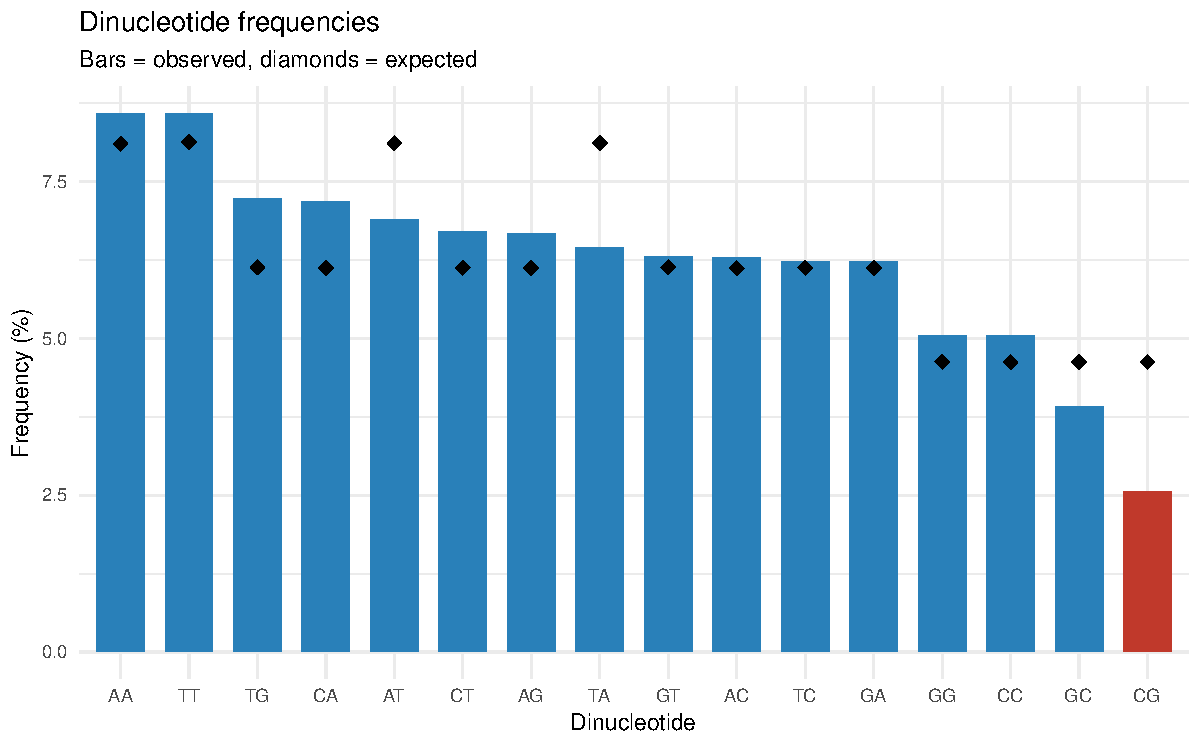
\includegraphics[width=\textwidth]{fig1a_dinucleotide_freq.pdf}
        \caption{}
    \end{subfigure}
    \hfill
    \begin{subfigure}[b]{0.48\textwidth}
        \centering
        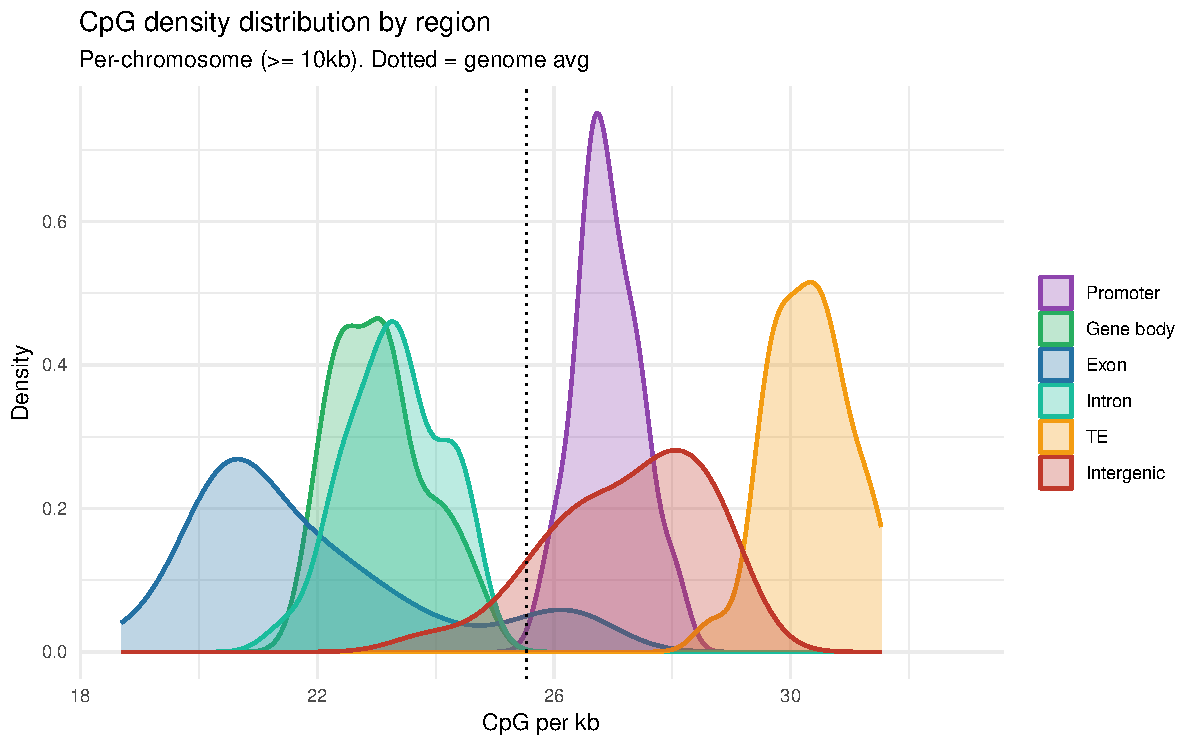
\includegraphics[width=\textwidth]{fig1b_cpg_density_distribution.pdf}
        \caption{}
    \end{subfigure}

    \vspace{0.5cm}

    \begin{subfigure}[b]{0.48\textwidth}
        \centering
        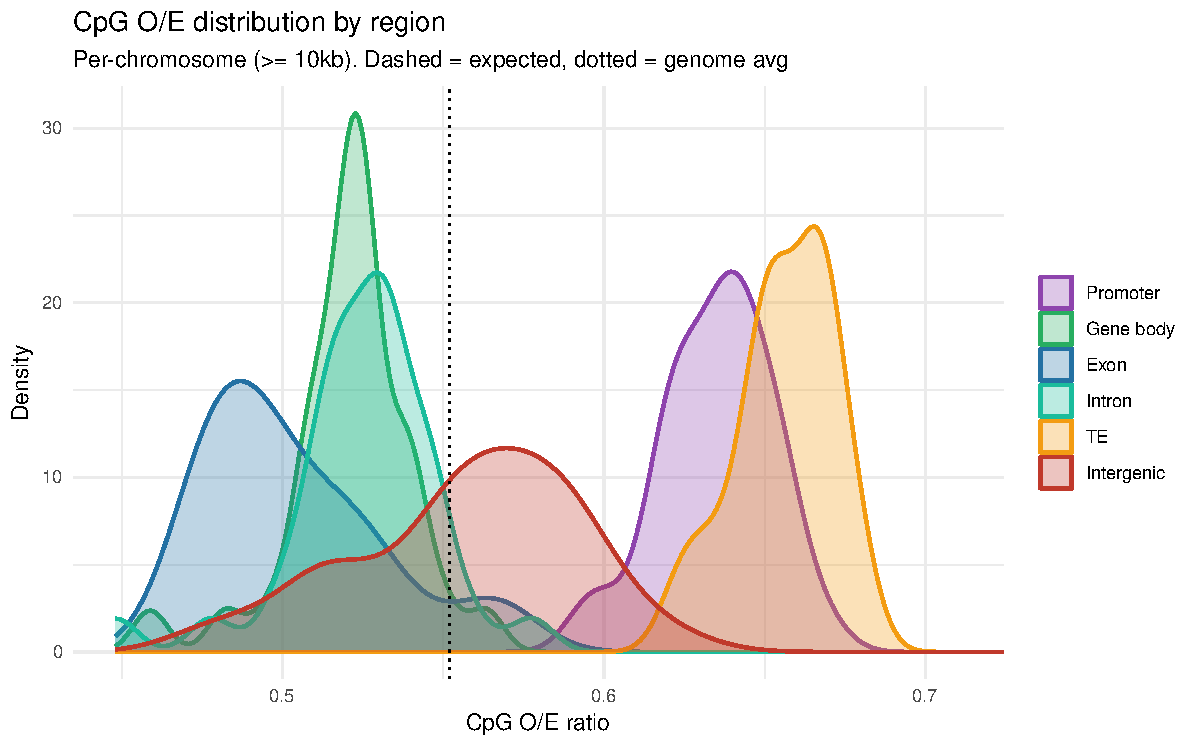
\includegraphics[width=\textwidth]{fig1c_cpg_oe_distribution.pdf}
        \caption{}
    \end{subfigure}
    \hfill
    \begin{subfigure}[b]{0.48\textwidth}
        \centering
        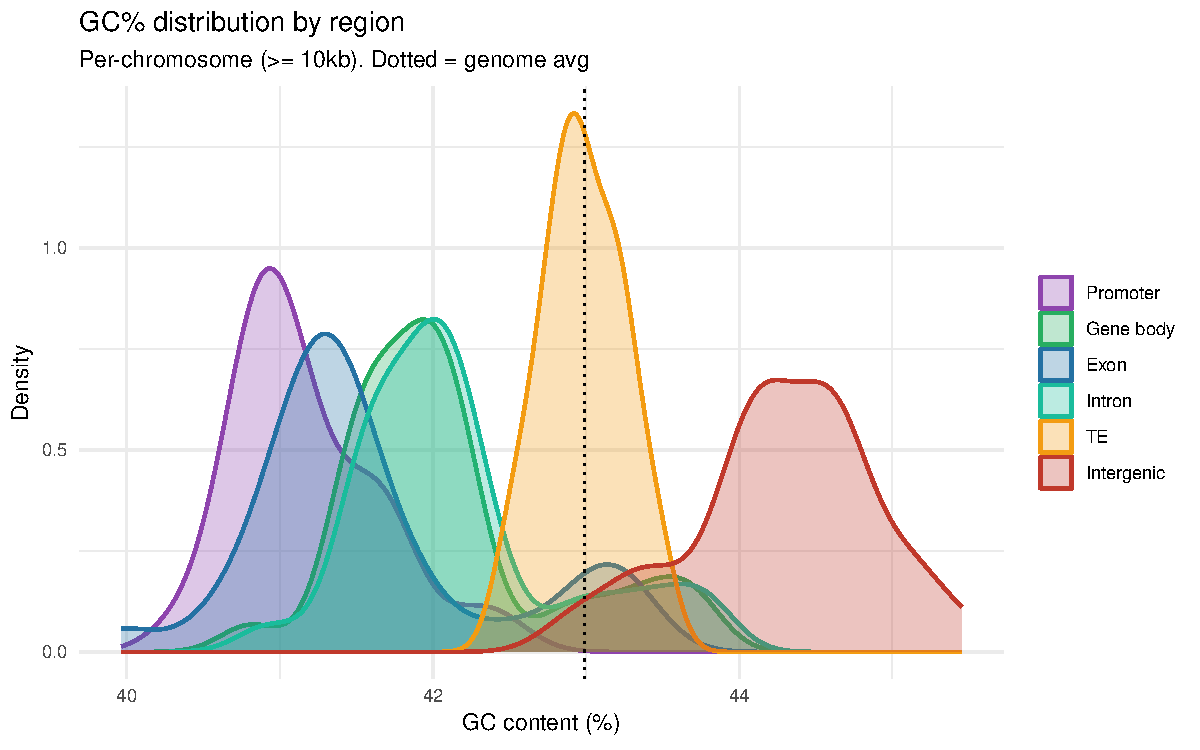
\includegraphics[width=\textwidth]{fig1d_gc_distribution.pdf}
        \caption{}
    \end{subfigure}

    \caption{\textbf{The \textit{D.\ laeve} genome displays CpG depletion consistent with historical cytosine methylation.}
    (\textbf{A}) Observed vs.\ expected dinucleotide frequencies across the genome; CpG is the most underrepresented dinucleotide (O/E = 0.553).
    (\textbf{B}) Distribution of CpG density across 1-kb genomic windows.
    (\textbf{C}) CpG observed/expected ratio distribution, showing unimodal depletion.
    (\textbf{D}) GC content distribution across 1-kb windows (genome-wide mean = 43.0\%).}
    \label{fig:deamination}
\end{figure}


%% =====================================================================
%% FIGURE 2 — METHYLATION TOOLKIT + EXPRESSION ACROSS TISSUES
%% =====================================================================

\subsection*{The methylation toolkit of \textit{D.\ laeve} lacks \textit{de novo} methyltransferases}

To characterize the enzymatic machinery available for establishing, maintaining, and reading DNA methylation in \textit{D.\ laeve}, we performed BLAST and HMMER searches of the predicted proteome against known DNMT, TET, and MBD-family proteins from vertebrate and invertebrate reference species.

We identified a single DNMT1 gene, the canonical maintenance methyltransferase, but found no homologues of the \textit{de novo} methyltransferases DNMT3A or DNMT3B, nor of DNMT2 (Fig.~\ref{fig:toolkit}A). Among active demethylation enzymes, we identified both TET2 and TET3 but not TET1, indicating that two TET-family dioxygenases are available for oxidation of 5mC. The genome encodes MBD2 and MBD4 methyl-CpG binding proteins but lacks MBD1, MBD3, and MeCP2 (Fig.~\ref{fig:toolkit}A). UHRF1---a cofactor essential for DNMT1 recruitment to hemimethylated DNA during replication---was present in two copies, and HELLS, a chromatin remodeler that functions as a cofactor for both DNMT3 and TET enzymes in mammals, was also duplicated. The base excision repair pathway was represented by APEX1, two copies of TDG, and three GADD45 paralogs. HDAC2, a histone deacetylase that can function in concert with MBD2, was also present.

The duplication of HELLS is particularly intriguing given the absence of its canonical partner DNMT3, raising the possibility that HELLS may participate in TET2/TET3-mediated demethylation or other chromatin remodeling functions in this organism. The absence of DNMT2, which is retained in many arthropods and vertebrates, further distinguishes the \textit{D.\ laeve} epigenetic toolkit.

Expression profiling of all 18 identified methylation machinery genes across six tissues---tail, eye, body wall, head, juvenile, and ovotestis---under control and experimental conditions revealed that DNMT1, TET2, TET3, and UHRF1 are broadly expressed, with no dramatic tissue-specific restriction (Fig.~\ref{fig:toolkit}B). DNMT1 expression was modestly but consistently detected across all tissues, consistent with its constitutive role in maintenance methylation. TET3 showed somewhat higher expression in the ovotestis, potentially reflecting elevated demethylation activity in the germline.

\begin{figure}[ht]
    \centering
    \begin{subfigure}[b]{0.45\textwidth}
        \centering
        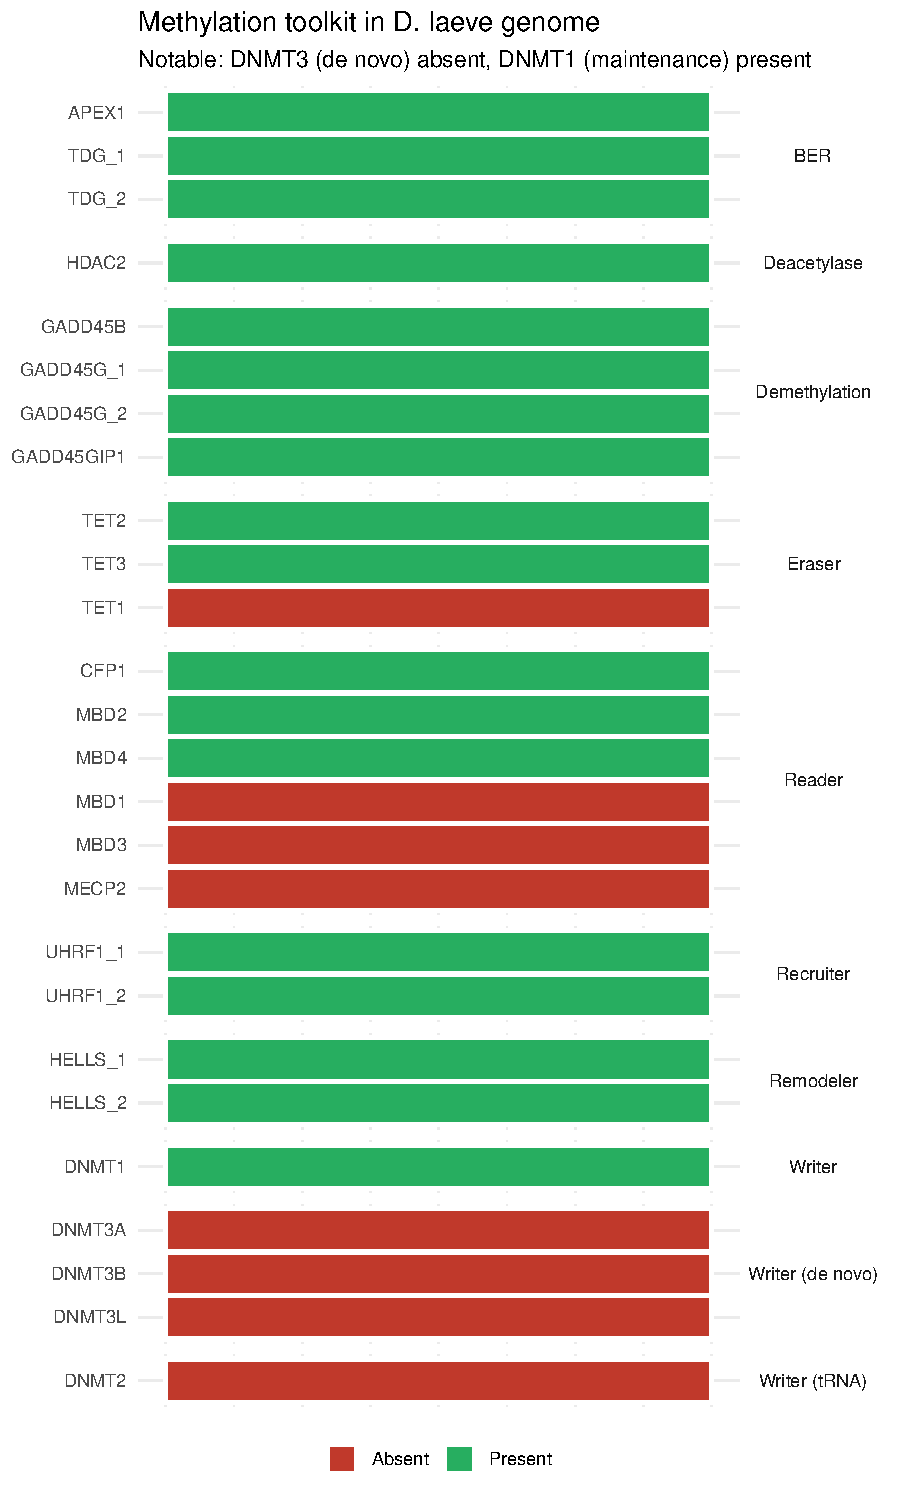
\includegraphics[width=\textwidth]{fig2a_methylation_toolkit_presence.pdf}
        \caption{}
    \end{subfigure}
    \hfill
    \begin{subfigure}[b]{0.52\textwidth}
        \centering
        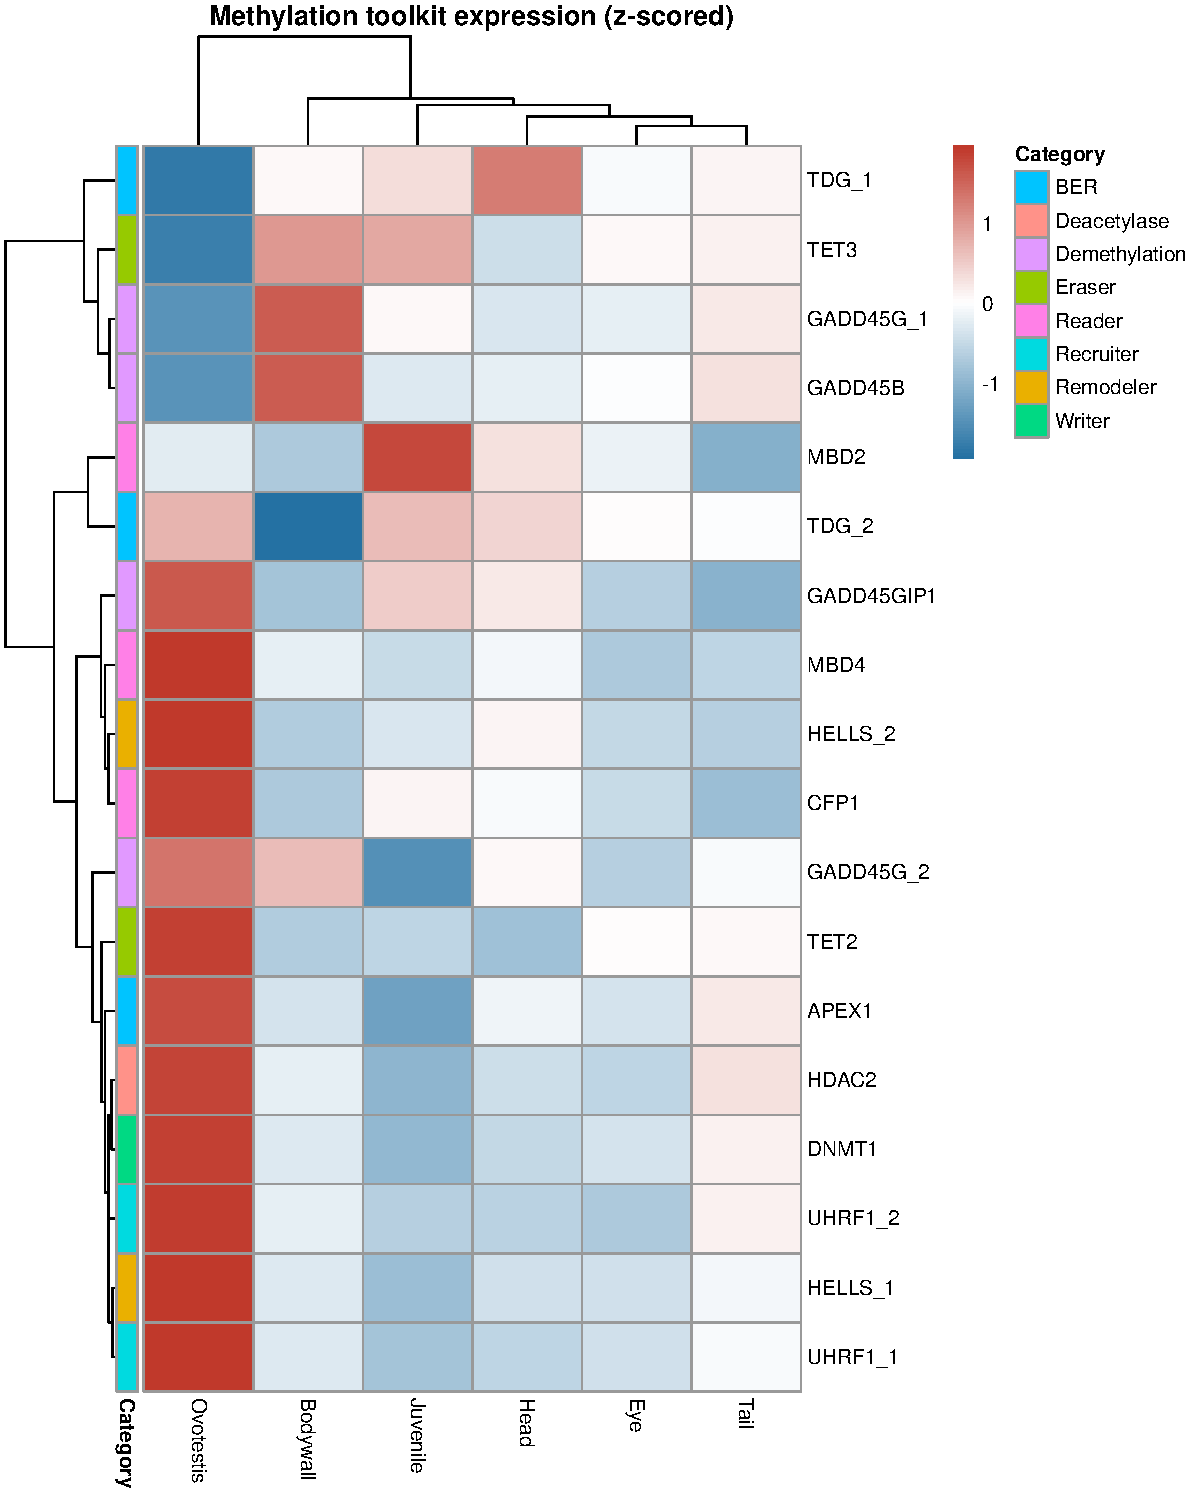
\includegraphics[width=\textwidth]{fig2c_methylation_toolkit_heatmap.pdf}
        \caption{}
    \end{subfigure}

    \caption{\textbf{The \textit{D.\ laeve} epigenetic toolkit retains maintenance methylation but lacks \textit{de novo} methyltransferases.}
    (\textbf{A}) Presence (green) and absence (red) of 26 methylation-related genes in \textit{D.\ laeve}, organized by functional category: 18 present, 8 absent (including DNMT3A/B/L, DNMT2, TET1, MBD1, MBD3, MeCP2).
    (\textbf{B}) Expression heatmap (z-scored VST) of all 18 present methylation machinery genes across tissues and conditions, with column annotations showing tissue identity and treatment status.}
    \label{fig:toolkit}
\end{figure}


%% =====================================================================
%% FIGURE 3 — MEAN METHYLATION, LANDSCAPE, CHROMOSOME VIEW
%% =====================================================================

\subsection*{Gene-body methylation dominates a mosaic methylome}

To establish the baseline methylation landscape of \textit{D.\ laeve}, we performed whole-genome bisulfite sequencing on tail tissue from two control and two amputated individuals. After alignment, deduplication, strand-collapse, and filtering for CpGs with $\geq$5$\times$ coverage in all four samples, we retained 25,439,068 CpG sites for downstream analysis.

Mean genome-wide CpG methylation was 18.1\% across all samples, with no global shift between control (C1: 18.1\%, C2: 18.0\%) and amputated (A1: 18.2\%, A2: 18.2\%) conditions (Fig.~\ref{fig:landscape}A). When methylation was partitioned by genomic region, promoters were consistently hypomethylated (mean 10.4\%), intergenic regions showed very low methylation (4.6\%), and gene bodies carried the bulk of methylation: exons at 48.7\% and introns at 26.9\% (Fig.~\ref{fig:landscape}B). Visualization of methylation across the genome in 1-Mb windows revealed a relatively uniform distribution across chromosomes, with no large-scale hypo- or hypermethylated chromosomal domains evident (Fig.~\ref{fig:landscape}C). This mosaic architecture---gene bodies methylated, promoters and intergenic regions hypomethylated---is consistent with the pattern described in other invertebrates.

\begin{figure}[ht]
    \centering
    \begin{subfigure}[b]{0.48\textwidth}
        \centering
        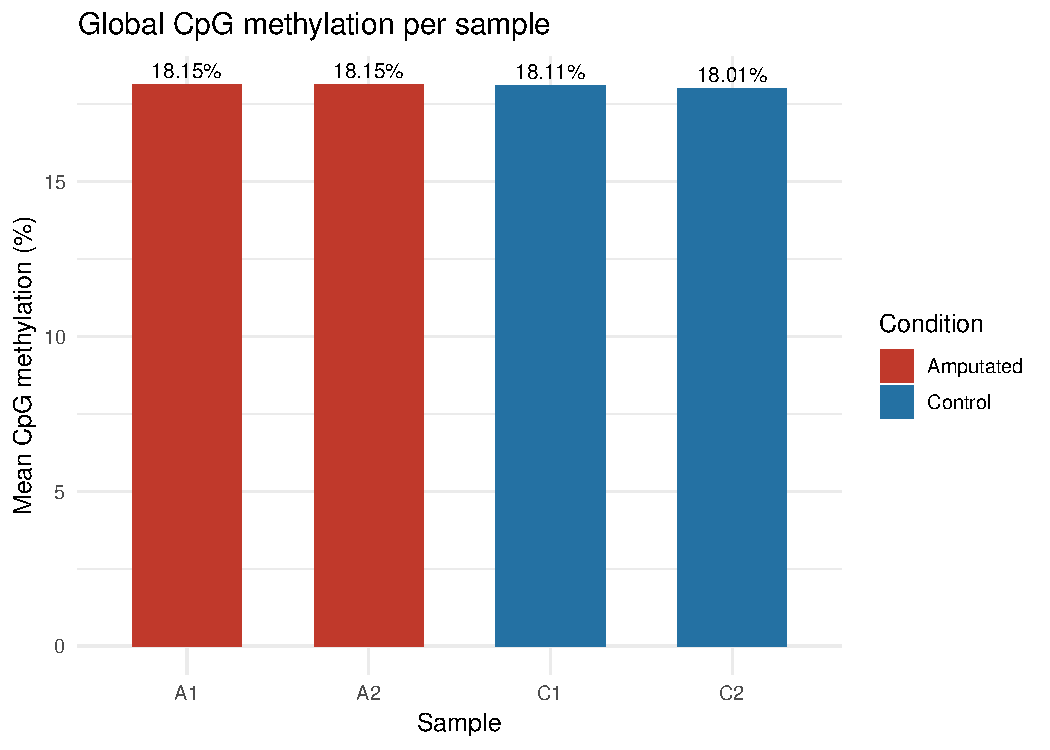
\includegraphics[width=\textwidth]{fig4a_global_methylation_per_sample.pdf}
        \caption{}
    \end{subfigure}
    \hfill
    \begin{subfigure}[b]{0.48\textwidth}
        \centering
        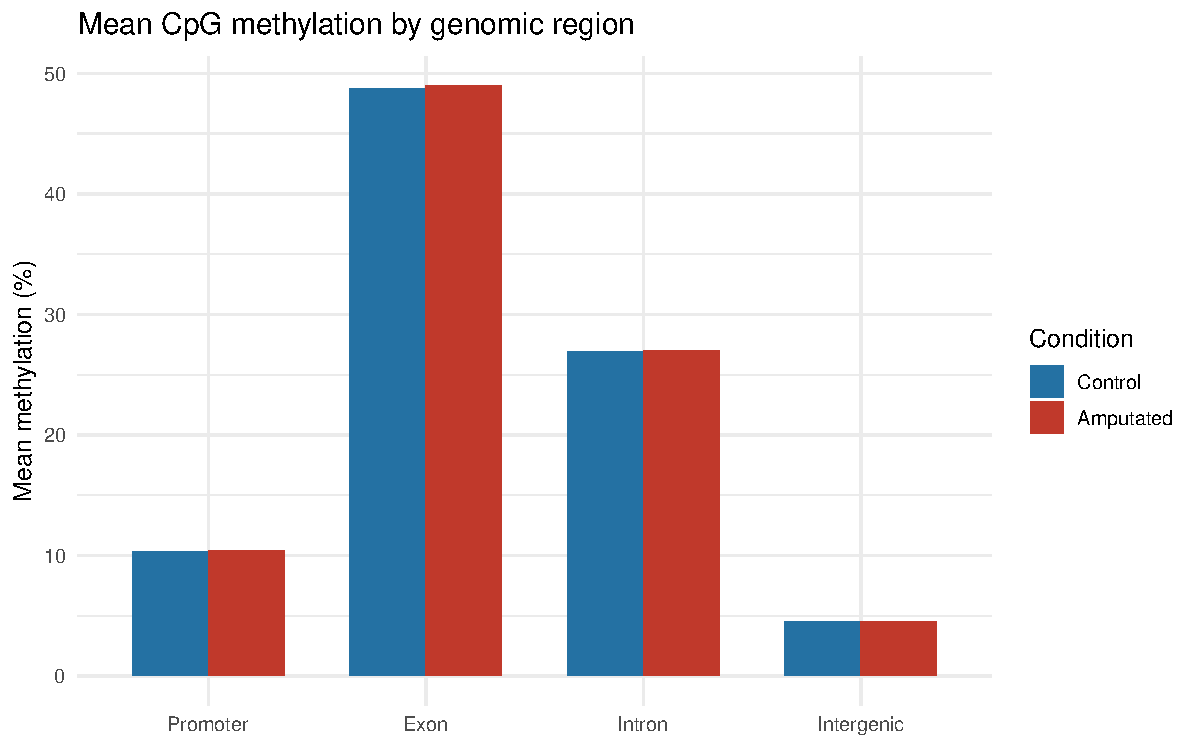
\includegraphics[width=\textwidth]{fig4c_region_methylation_bar.pdf}
        \caption{}
    \end{subfigure}

    \vspace{0.5cm}

    \begin{subfigure}[b]{0.95\textwidth}
        \centering
        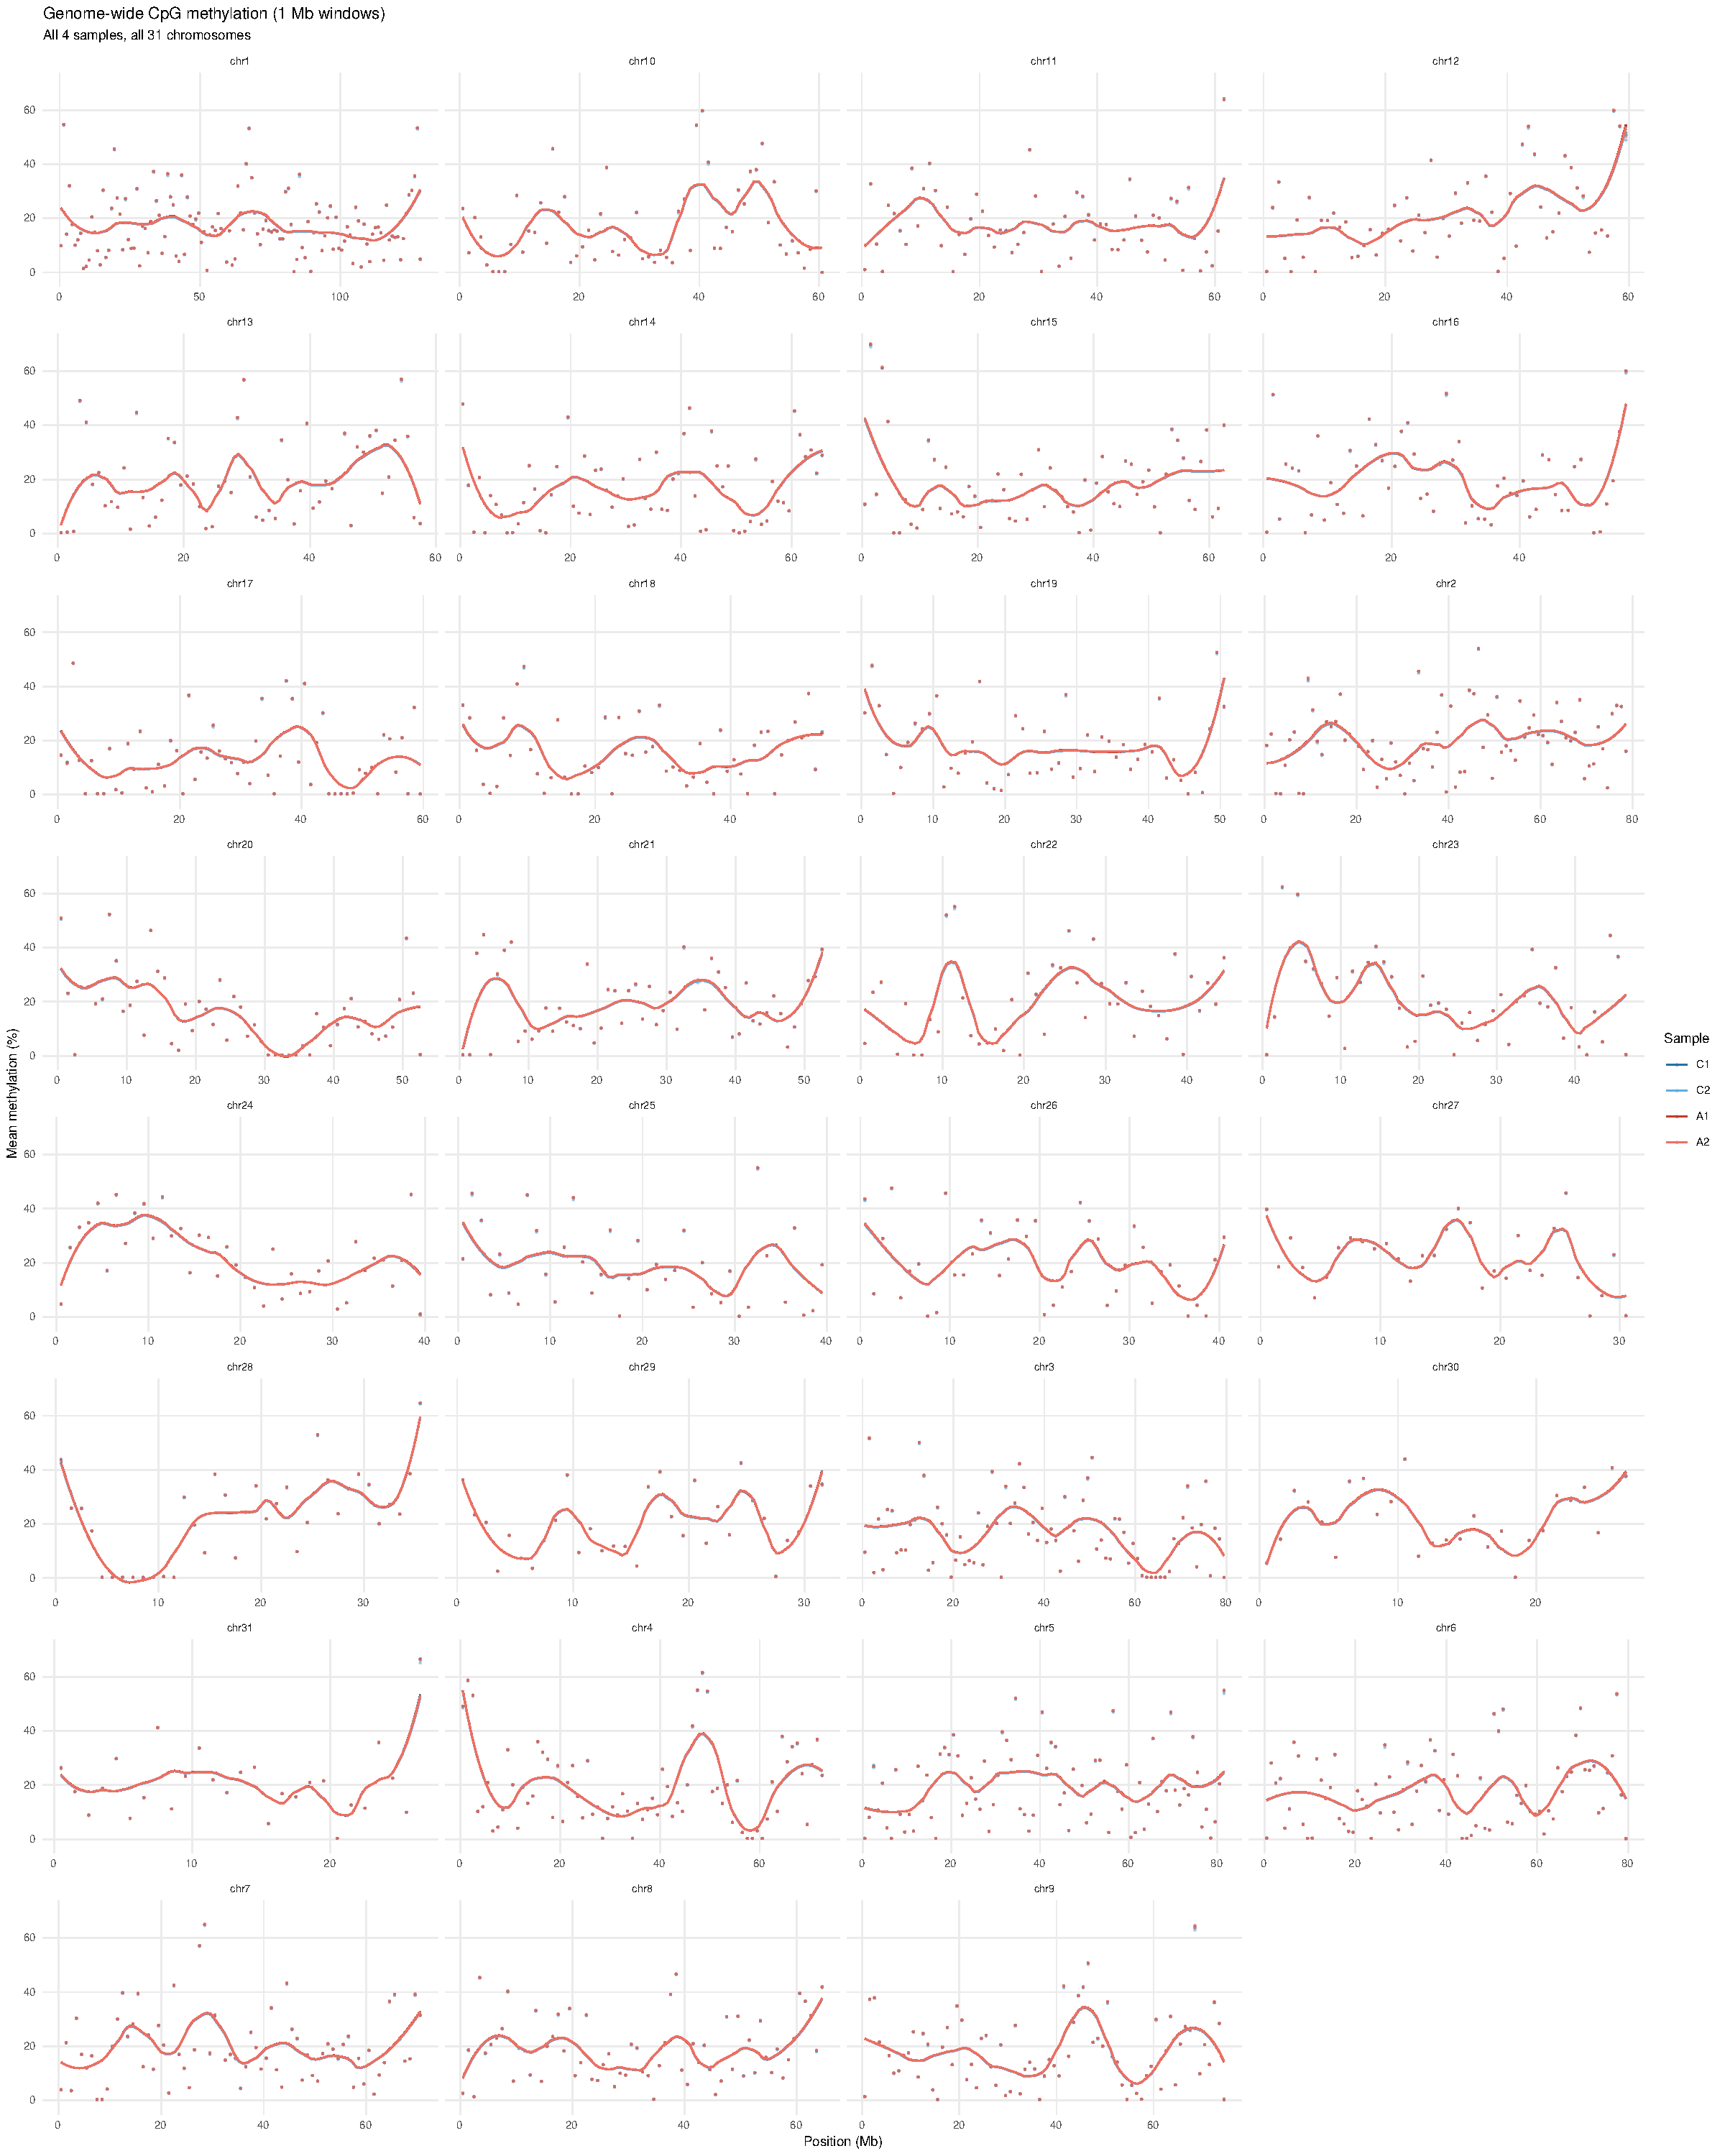
\includegraphics[width=\textwidth]{fig4i_genomewide_methylation_1mb.pdf}
        \caption{}
    \end{subfigure}

    \caption{\textbf{Gene-body methylation dominates a mosaic methylome in \textit{D.\ laeve}.}
    (\textbf{A}) Mean genome-wide CpG methylation per sample (control: blue; amputated: red). All four samples cluster near 18\%.
    (\textbf{B}) Mean methylation by genomic region (promoter, exon, intron, intergenic) for control and amputated conditions.
    (\textbf{C}) Genome-wide methylation landscape in 1-Mb windows across all 31 chromosomes, all 4 samples overlaid.}
    \label{fig:landscape}
\end{figure}


%% =====================================================================
%% FIGURE 4 — METAGENE + GENE BODY METH vs EXPRESSION
%% =====================================================================

\subsection*{Metagene methylation profiles reveal expression-dependent gene body methylation}

To examine how methylation is distributed across gene structures, we computed metagene methylation profiles by dividing each gene into four segments---distal upstream (5--2~kb), promoter (2~kb), gene body, and downstream (5~kb)---each split into 20 equal bins. Genes were stratified by expression level (deciles from RNA-seq) and by gene architecture (single-exon, 2-exon, 3+ exon).

Across all genes, the metagene profile showed a characteristic pattern of low promoter methylation, a sharp increase at the transcription start site, elevated methylation throughout the gene body, and a decline at the 3' end. Critically, gene body methylation scaled with expression level: the highest-expressed decile showed the highest gene body methylation, consistent with the invertebrate paradigm of gene body methylation marking constitutively active genes (Fig.~\ref{fig:metagene}A,~B). In genes with three or more exons, the gene-body signal showed a distinctive oscillating pattern, with methylation peaks corresponding to exonic bins and troughs at intronic bins (Fig.~\ref{fig:metagene}C,~D). This exon--intron oscillation was absent in intronless genes, which showed a smooth, elevated methylation plateau (Fig.~\ref{fig:metagene}E,~F).

Baseline gene body methylation was positively correlated with expression across all genes (Spearman $\rho = 0.407$, $p < 10^{-80}$, $n = 16{,}958$), with the strongest correlation in exonic regions ($\rho = 0.407$) and the weakest in promoters ($\rho = -0.015$) (Fig.~\ref{fig:methexpr}A,~B).

\begin{figure}[ht]
    \centering
    \begin{subfigure}[b]{0.48\textwidth}
        \centering
        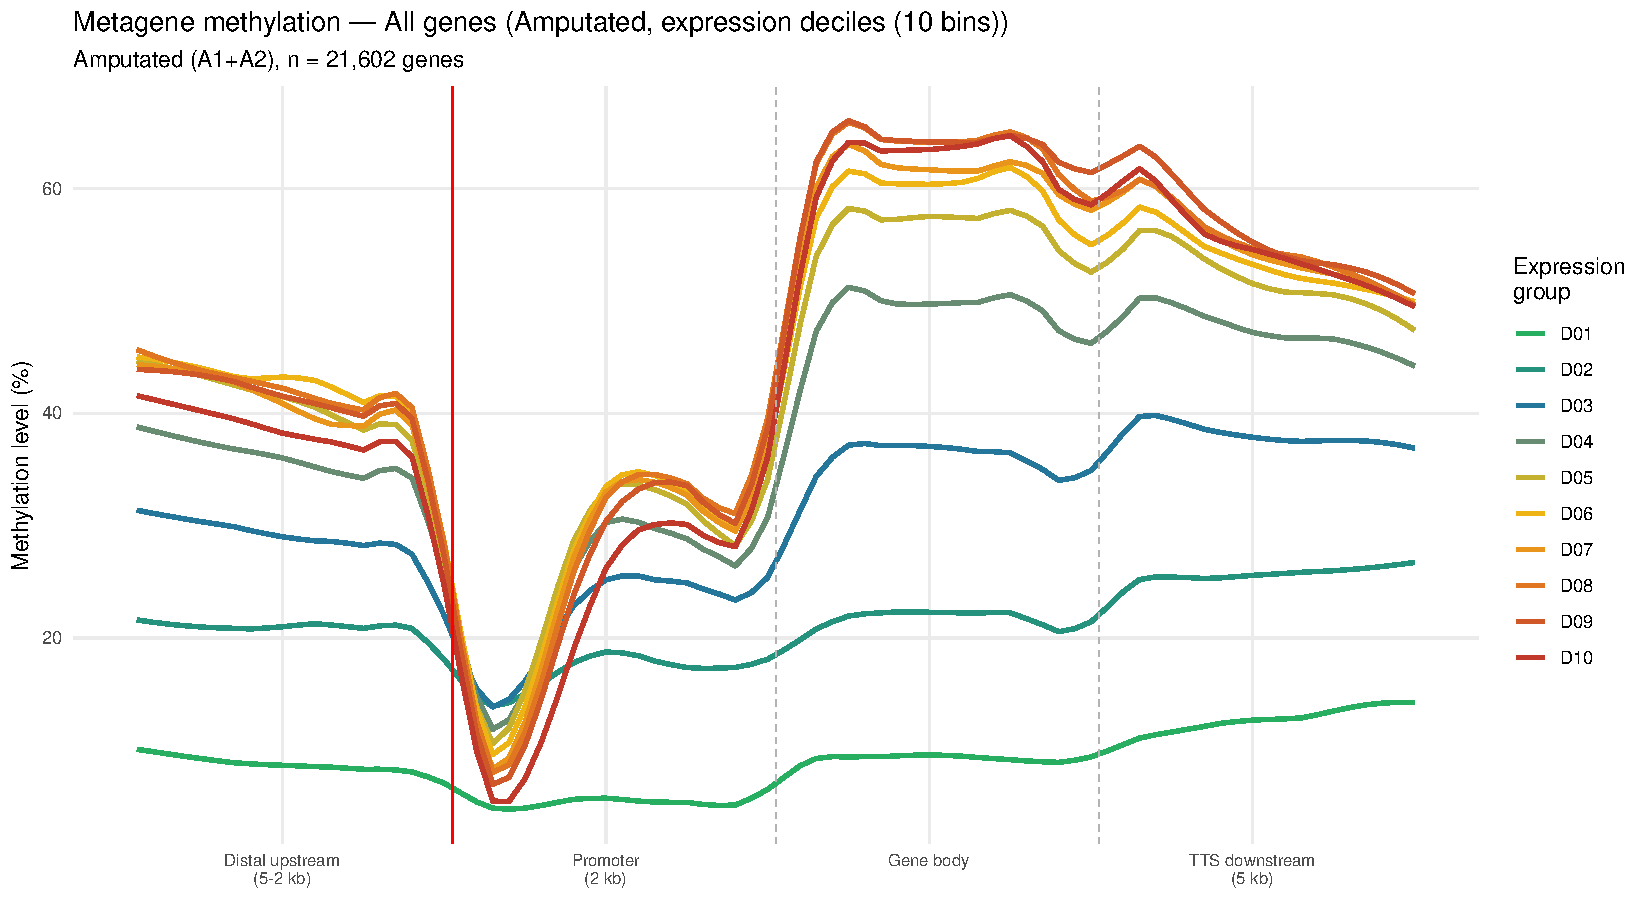
\includegraphics[width=\textwidth]{fig4d_bin10_01_ampu_all_genes.pdf}
        \caption{}
    \end{subfigure}
    \hfill
    \begin{subfigure}[b]{0.48\textwidth}
        \centering
        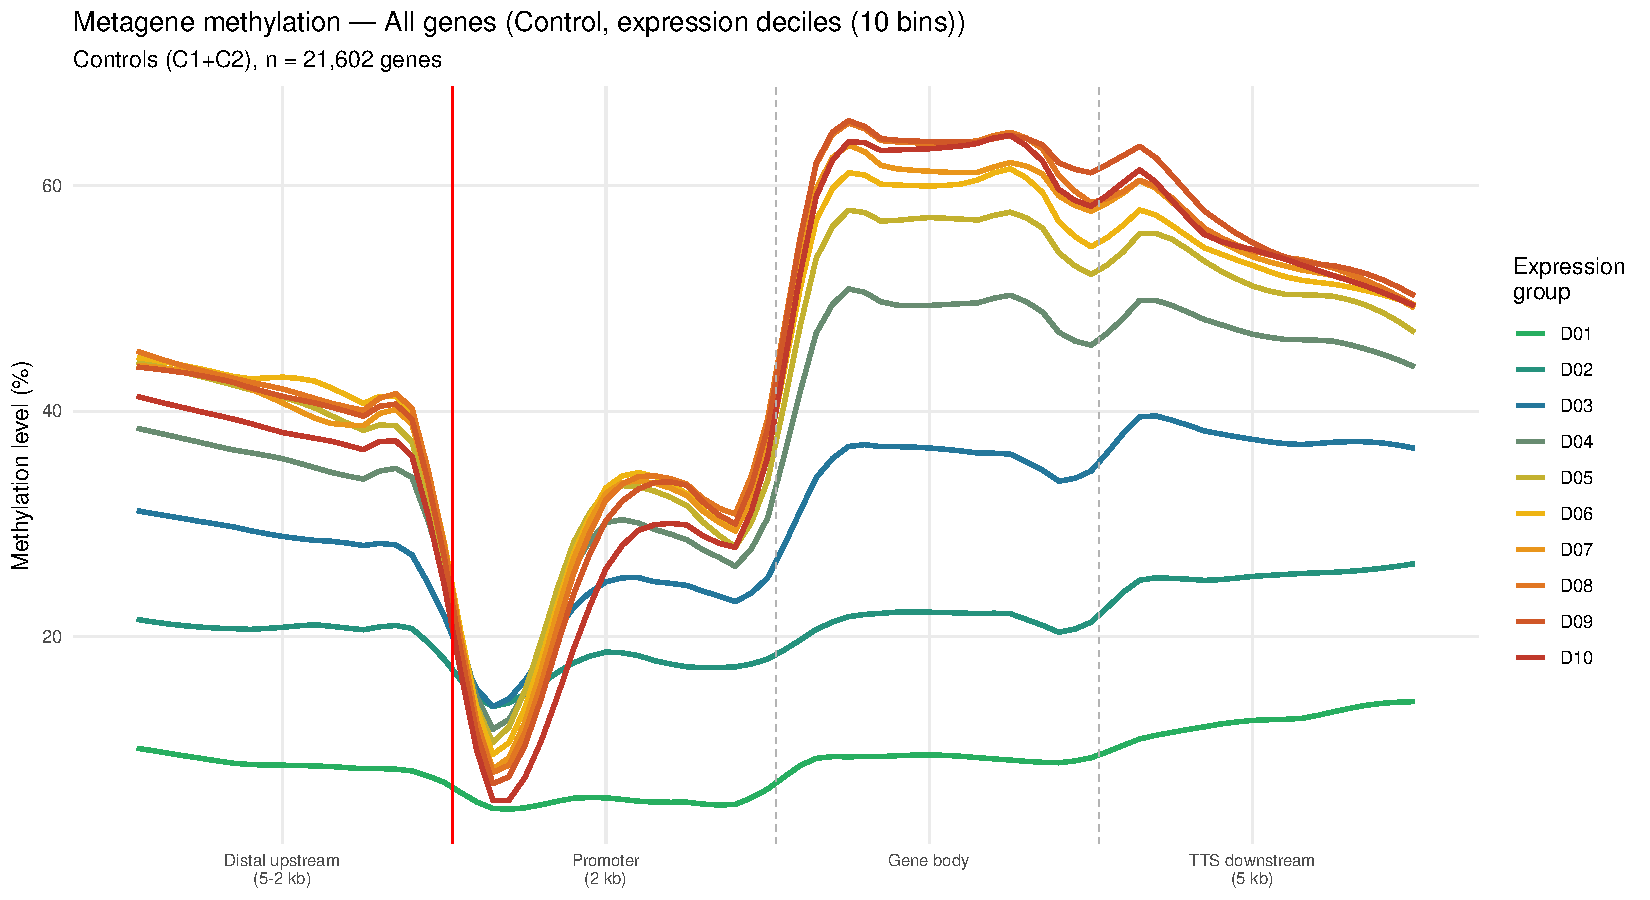
\includegraphics[width=\textwidth]{fig4d_bin10_02_ctrl_all_genes.pdf}
        \caption{}
    \end{subfigure}

    \vspace{0.5cm}

    \begin{subfigure}[b]{0.48\textwidth}
        \centering
        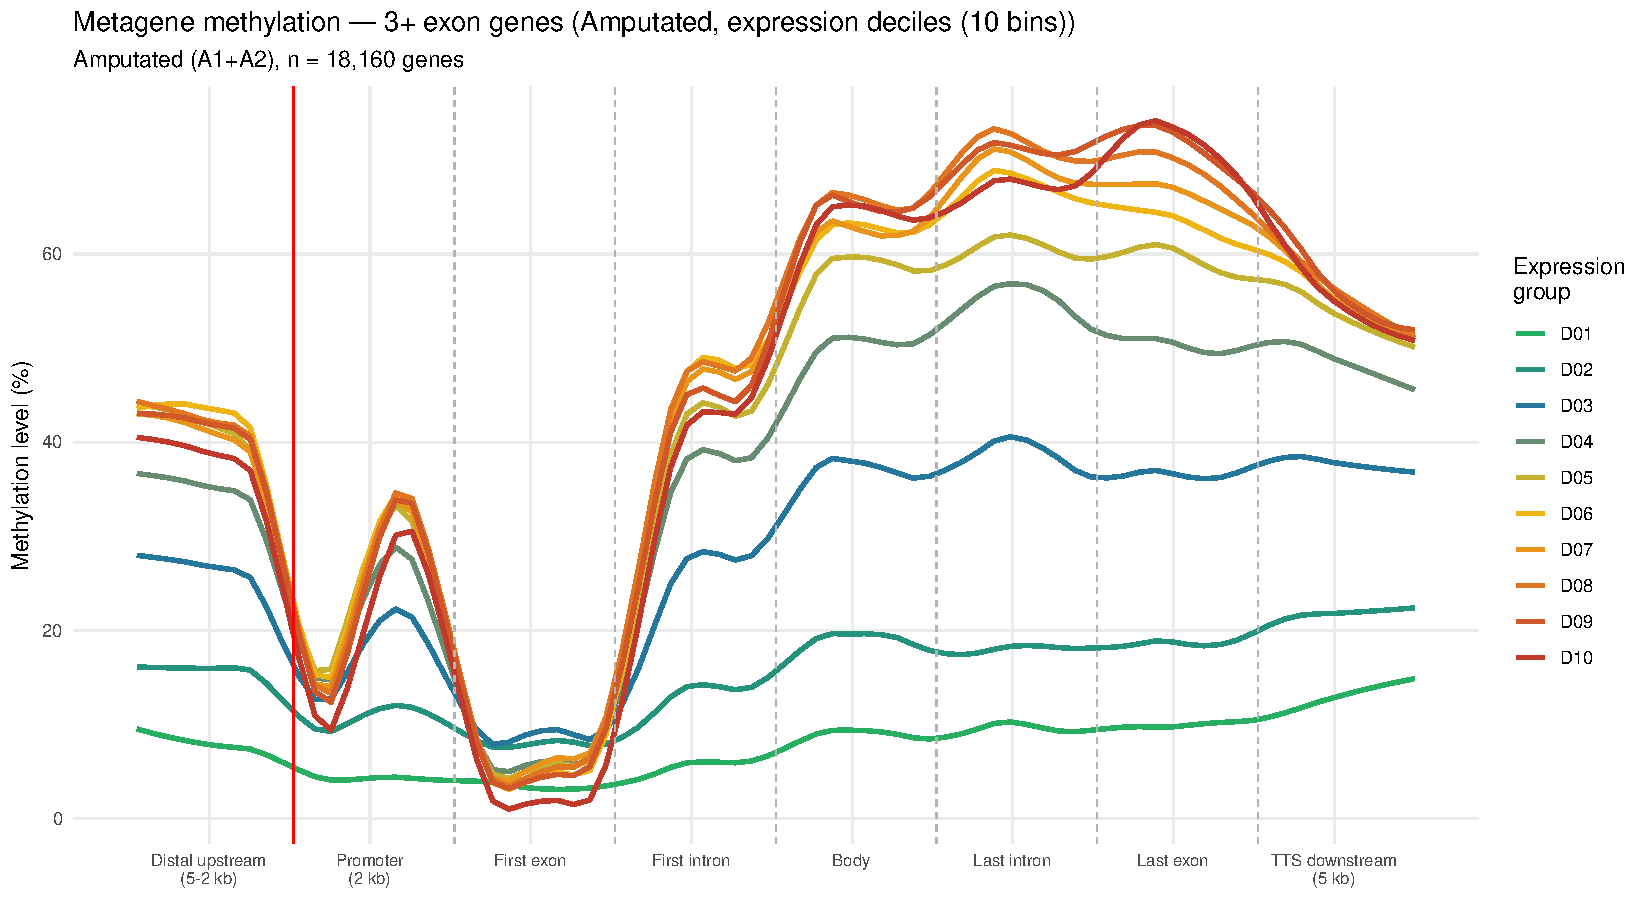
\includegraphics[width=\textwidth]{fig4d_bin10_03_ampu_3plus_exon.pdf}
        \caption{}
    \end{subfigure}
    \hfill
    \begin{subfigure}[b]{0.48\textwidth}
        \centering
        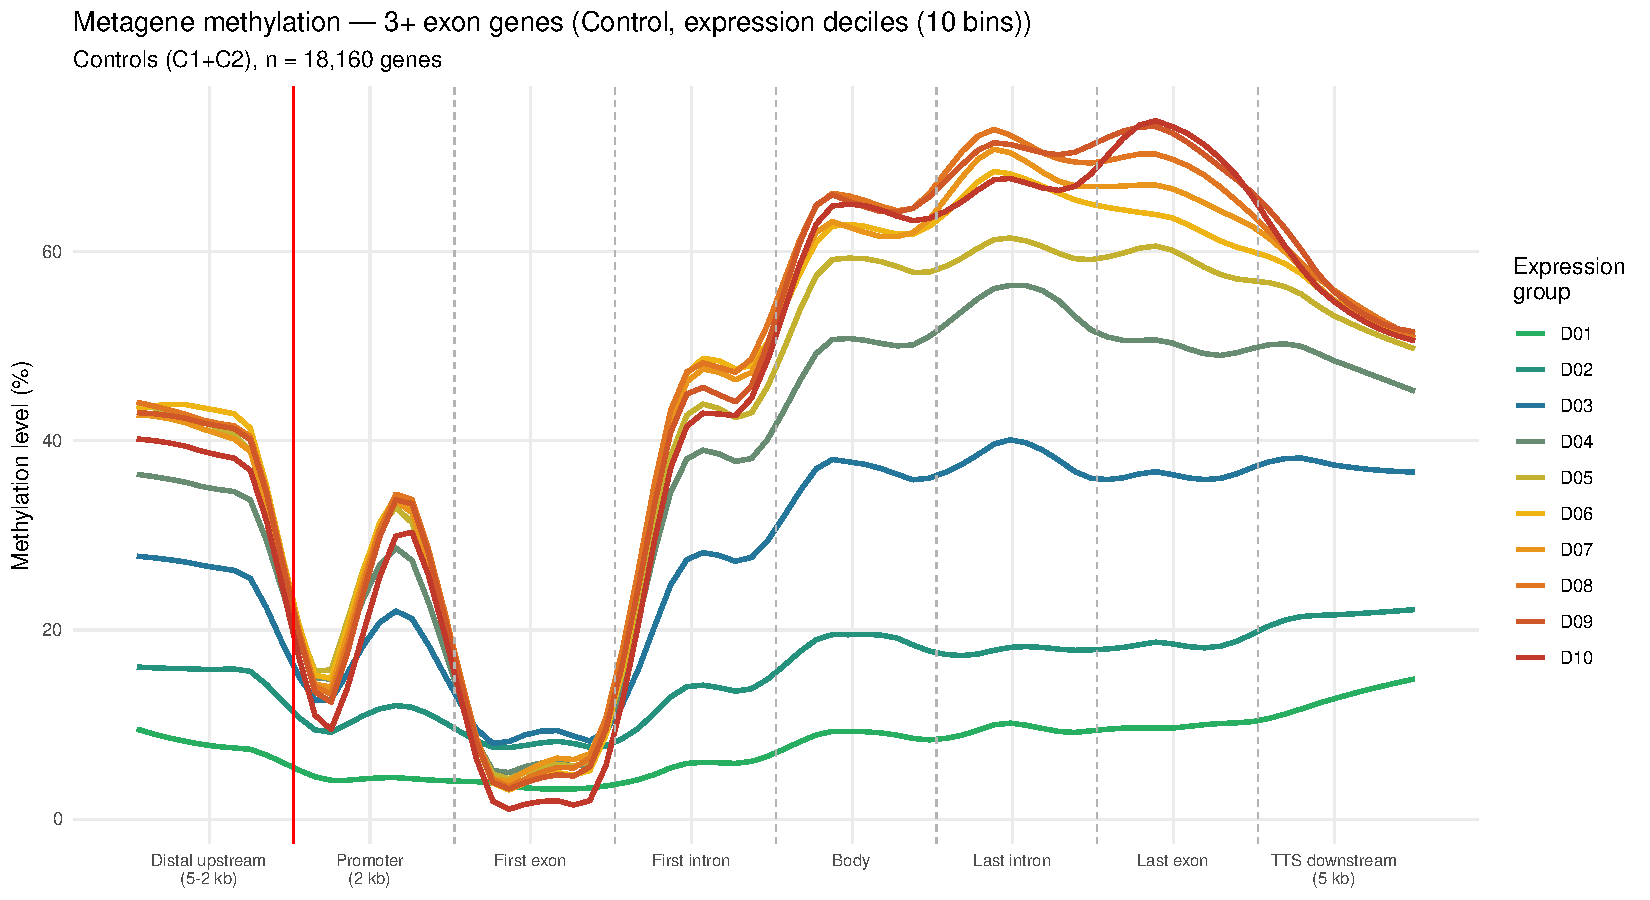
\includegraphics[width=\textwidth]{fig4d_bin10_04_ctrl_3plus_exon.pdf}
        \caption{}
    \end{subfigure}

    \vspace{0.5cm}

    \begin{subfigure}[b]{0.48\textwidth}
        \centering
        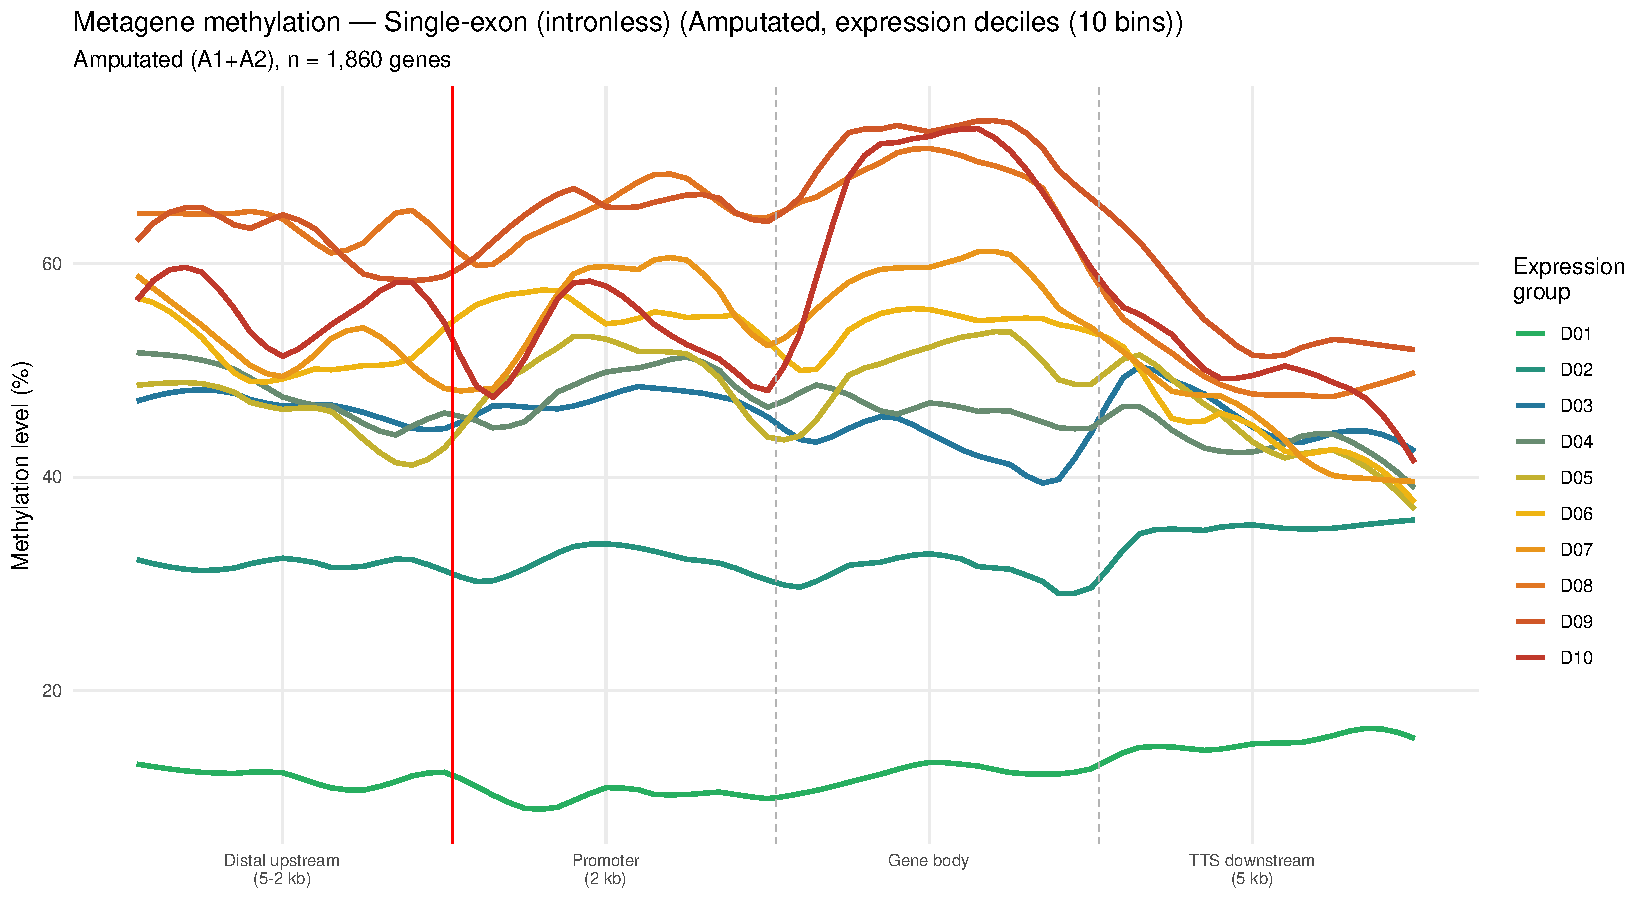
\includegraphics[width=\textwidth]{fig4d_bin10_07_ampu_single_exon.pdf}
        \caption{}
    \end{subfigure}
    \hfill
    \begin{subfigure}[b]{0.48\textwidth}
        \centering
        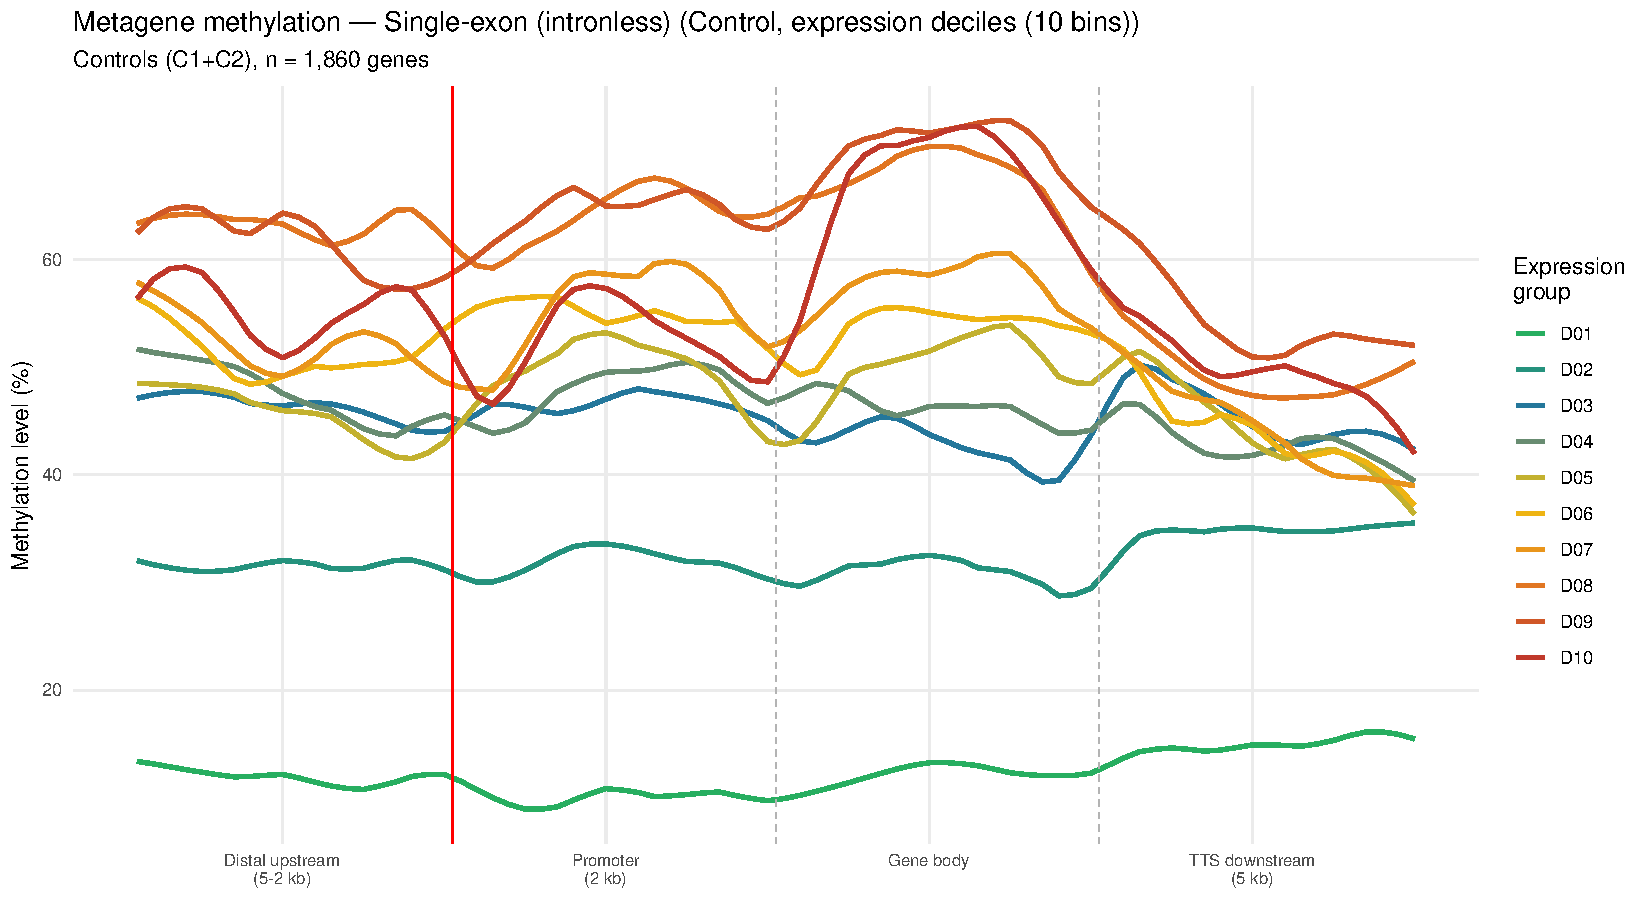
\includegraphics[width=\textwidth]{fig4d_bin10_08_ctrl_single_exon.pdf}
        \caption{}
    \end{subfigure}

    \caption{\textbf{Metagene methylation profiles across gene architecture classes.}
    (\textbf{A},~\textbf{B}) All genes, amputated and control, colored by expression decile (red = highest, green = lowest).
    (\textbf{C},~\textbf{D}) Genes with $\geq$3 exons, showing exon--intron methylation oscillation.
    (\textbf{E},~\textbf{F}) Intronless (single-exon) genes, showing smooth gene-body methylation.
    Metagene profiles span distal upstream (5--2~kb), promoter (2~kb), gene body (20 bins), and downstream (5~kb).}
    \label{fig:metagene}
\end{figure}

\begin{figure}[ht]
    \centering
    \begin{subfigure}[b]{0.48\textwidth}
        \centering
        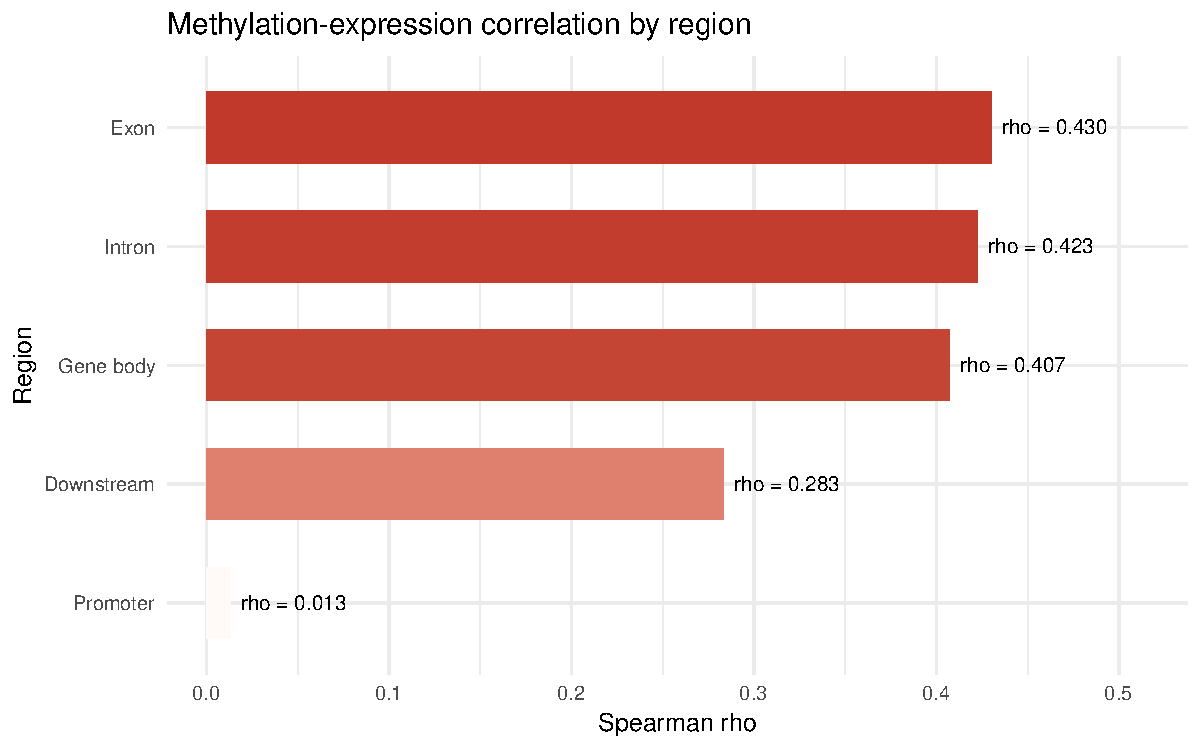
\includegraphics[width=\textwidth]{fig4f_region_meth_expression_correlation.pdf}
        \caption{}
    \end{subfigure}
    \hfill
    \begin{subfigure}[b]{0.48\textwidth}
        \centering
        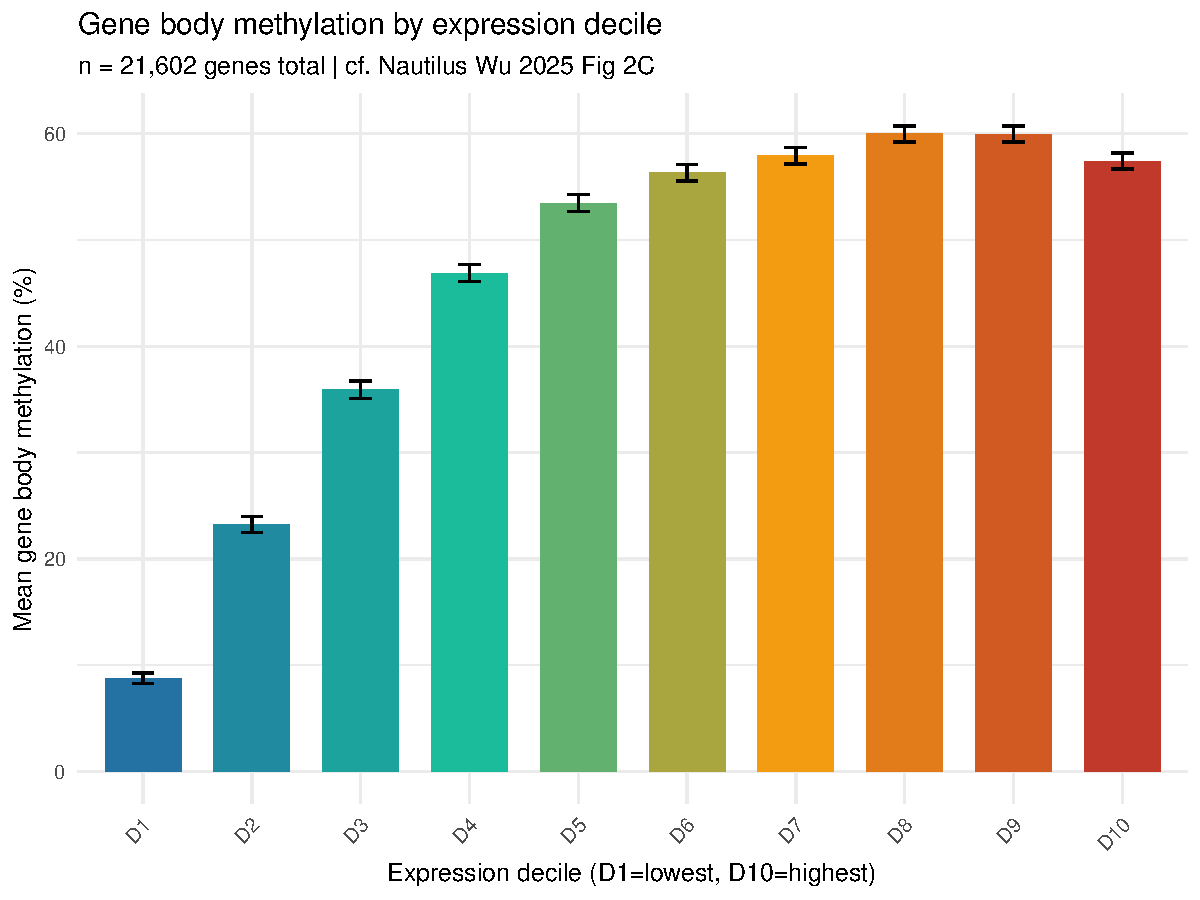
\includegraphics[width=\textwidth]{fig4g_meth_by_expression_decile.pdf}
        \caption{}
    \end{subfigure}

    \caption{\textbf{Gene body methylation correlates with expression at baseline.}
    (\textbf{A}) Methylation--expression Spearman correlation by genomic region.
    (\textbf{B}) Mean gene body methylation by expression decile (D1=lowest, D10=highest).}
    \label{fig:methexpr}
\end{figure}


%% =====================================================================
%% FIGURE 5 — TRANSPOSABLE ELEMENT METHYLATION
%% =====================================================================

\subsection*{Transposable elements show moderate, context-dependent methylation}

In mammals, DNA methylation serves as a primary defense mechanism against transposable element (TE) activity, with approximately 80\% of CpG methylation occurring at repetitive elements. To determine whether \textit{D.\ laeve} follows a similar pattern, we analyzed methylation levels across TE superfamilies annotated by RepeatMasker and stratified by genomic context.

TE methylation in \textit{D.\ laeve} was moderate, with most TE classes showing mean methylation levels between 20\% and 40\%---substantially lower than the near-complete methylation typically observed at mammalian TEs (Fig.~\ref{fig:te}A). The distribution of methylation across individual TE copies was broad and varied by superfamily: DNA transposons and LTR retrotransposons showed the widest distributions, while SINEs were more uniformly low. When TEs were stratified by genomic context, TEs overlapping gene bodies showed significantly higher methylation than intergenic TEs (Fig.~\ref{fig:te}B), suggesting that at least part of the TE methylation signal may be a byproduct of gene-body methylation rather than targeted silencing. Methylation also varied with TE evolutionary age (estimated from Kimura divergence): younger TEs tended to show lower methylation regardless of class, while older TEs embedded within genes showed the highest methylation levels (Fig.~\ref{fig:te}C).

\begin{figure}[ht]
    \centering
    \begin{subfigure}[b]{0.48\textwidth}
        \centering
        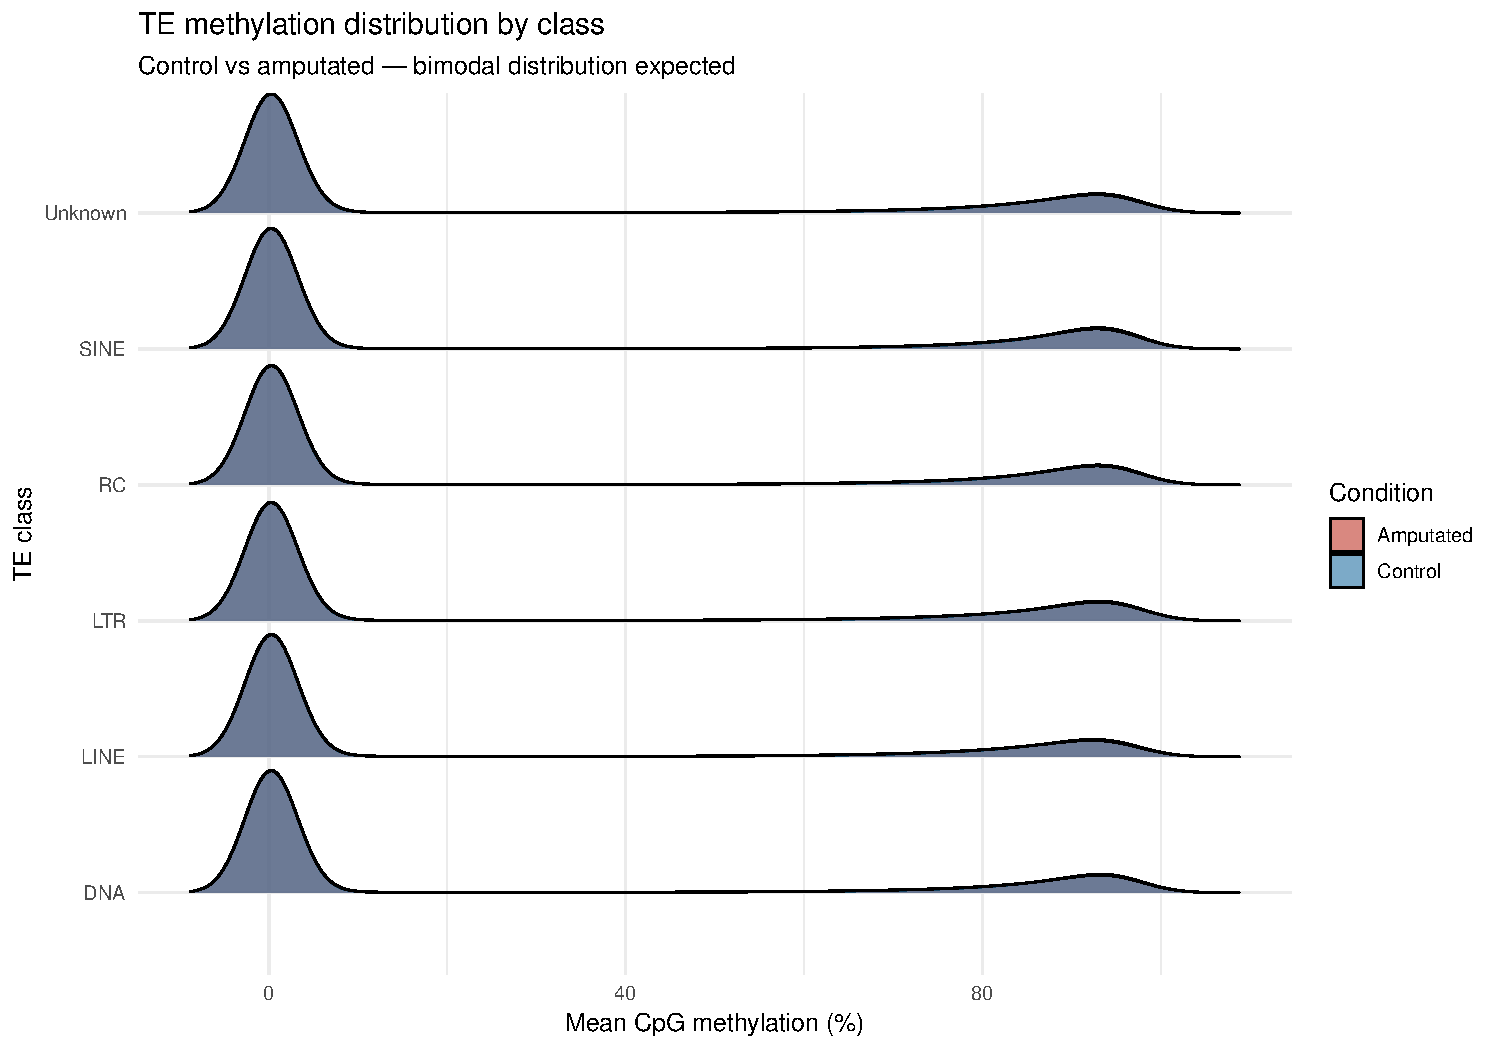
\includegraphics[width=\textwidth]{fig5a_te_ridge_by_class.pdf}
        \caption{}
    \end{subfigure}
    \hfill
    \begin{subfigure}[b]{0.48\textwidth}
        \centering
        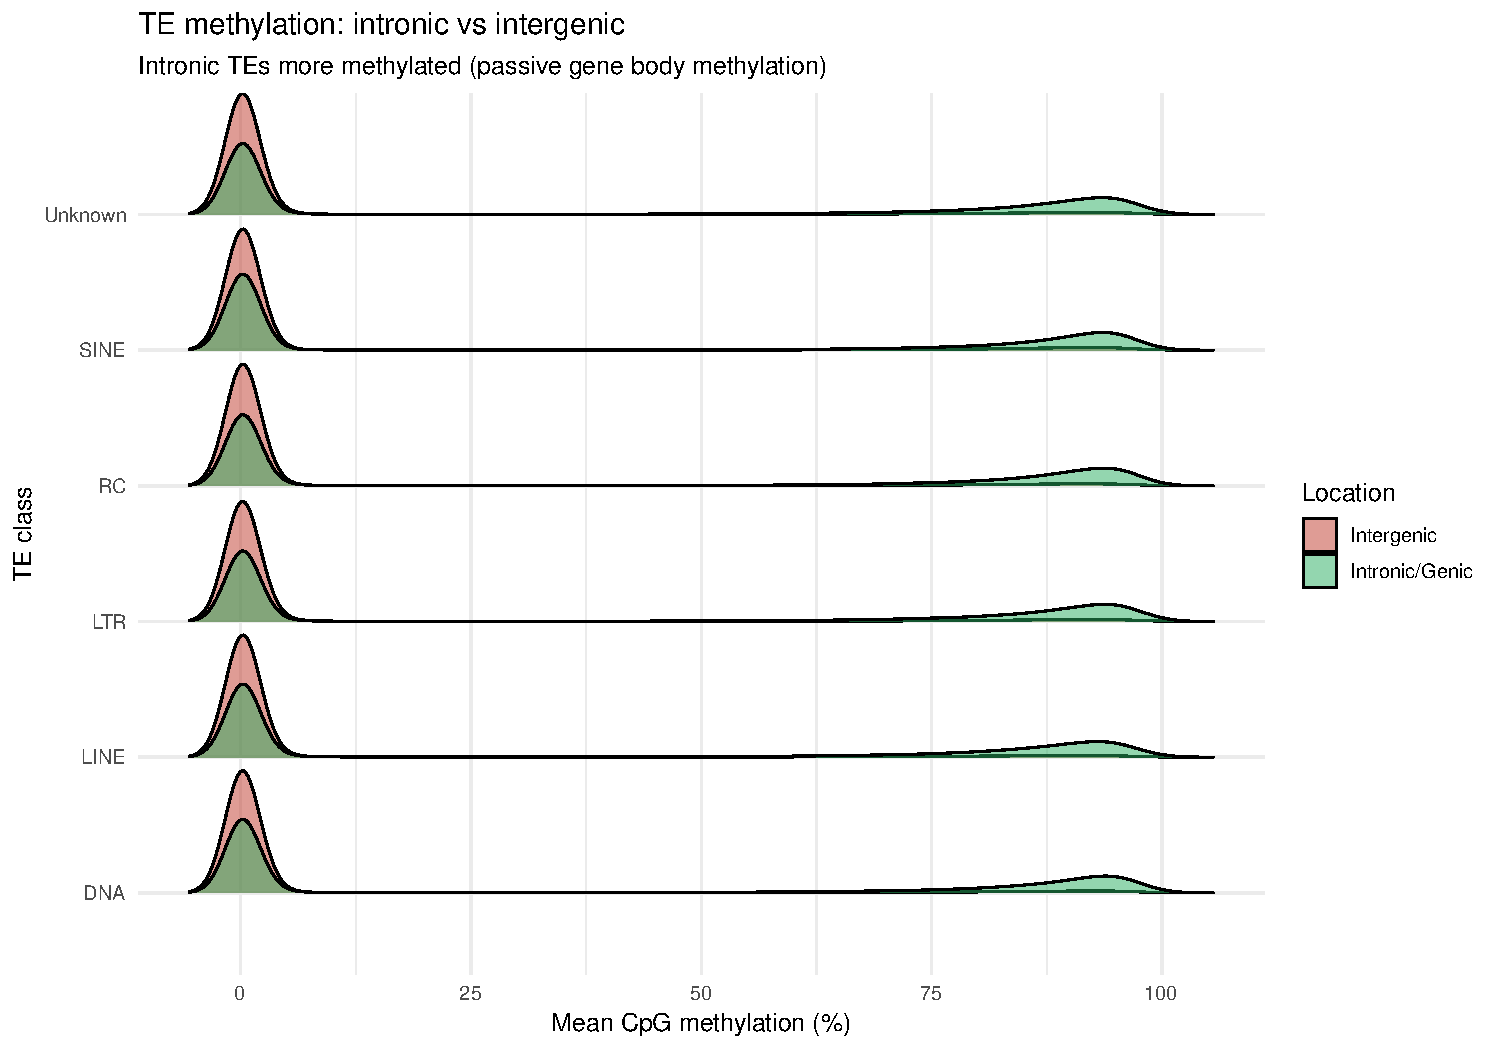
\includegraphics[width=\textwidth]{fig5b_te_intronic_vs_intergenic_ridge.pdf}
        \caption{}
    \end{subfigure}

    \vspace{0.5cm}

    \begin{subfigure}[b]{0.95\textwidth}
        \centering
        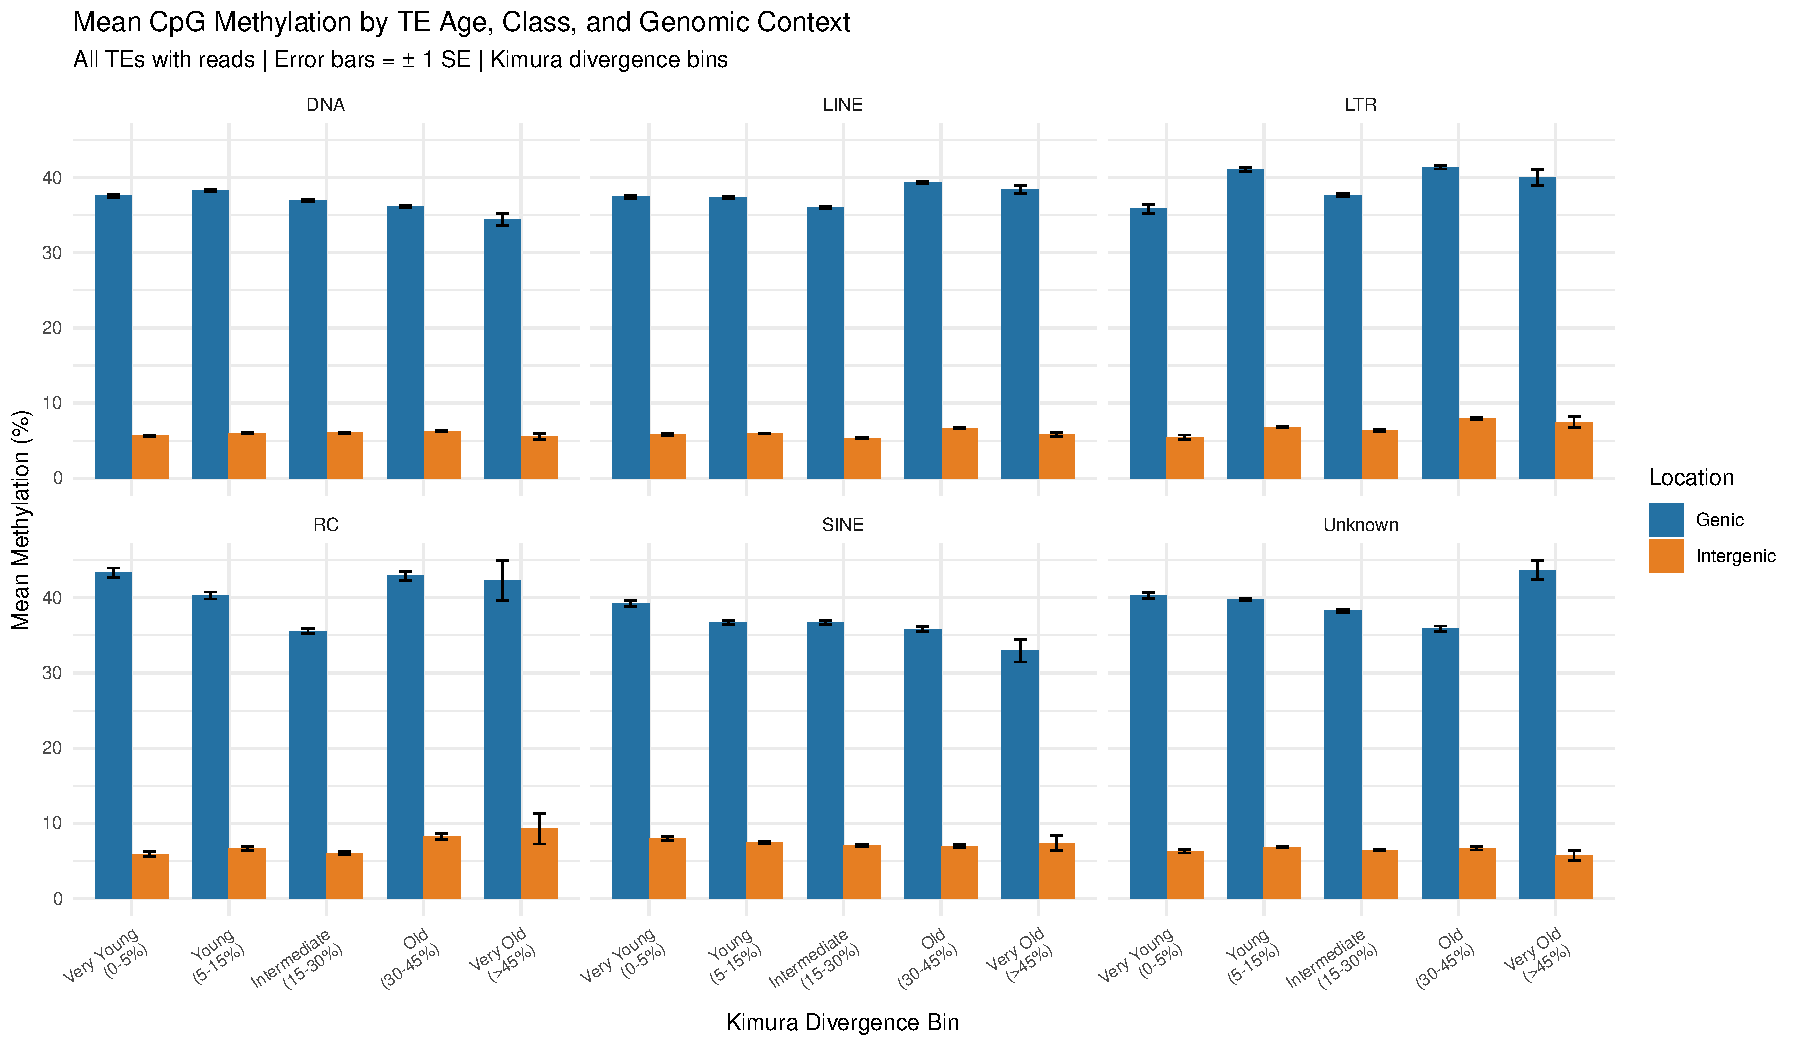
\includegraphics[width=\textwidth]{fig5g_te_age_bar.pdf}
        \caption{}
    \end{subfigure}

    \caption{\textbf{Transposable elements display moderate, context-dependent methylation.}
    (\textbf{A}) Ridge plot of per-copy methylation levels by TE superfamily, shown separately for control and amputated conditions.
    (\textbf{B}) TE methylation stratified by genomic context (overlapping genes vs.\ intergenic), showing higher methylation for TEs embedded within gene bodies.
    (\textbf{C}) Mean TE methylation by Kimura divergence age bin, TE class, and genomic context.}
    \label{fig:te}
\end{figure}


%% =====================================================================
%% FIGURE 6 — DIFFERENTIAL METHYLATION
%% =====================================================================

\subsection*{Amputation induces widespread but modest methylation changes}

To identify methylation changes associated with regeneration, we performed differential methylation analysis using DSS, comparing amputated (2~dpa blastema) and control (unamputated tail) samples. We identified 17,729 differentially methylated positions (DMPs; FDR $< 0.05$, $|\Delta\beta| > 10\%$) and 1,462 differentially methylated regions (DMRs) at a false discovery rate below 0.05.

The DMP distribution was roughly balanced between hypermethylated (8,285; 46.7\%) and hypomethylated (9,444; 53.3\%) sites in the amputated condition (Fig.~\ref{fig:differential}A). DMRs were similarly balanced (690 hyper, 772 hypo; Fig.~\ref{fig:differential}B). Among the genes carrying the highest DMP burden---defined as the number of significant DMPs per gene---several encoded proteins involved in cell adhesion, extracellular matrix remodeling, and cytoskeletal organization (Fig.~\ref{fig:differential}C). A similar pattern emerged for genes with the highest DMR burden (Fig.~\ref{fig:differential}D).

Gene Ontology enrichment analysis of all DMP-associated genes revealed significant overrepresentation of terms related to ciliary architecture, cell projection organization, morphogenesis, and cytoskeletal dynamics (Fig.~\ref{fig:differential}E). These functional categories are consistent with the cellular processes expected during blastema formation and tissue remodeling and suggest that methylation changes, while modest in magnitude, are not randomly distributed across the genome but target functionally coherent gene sets relevant to regeneration.

\begin{figure}[ht]
    \centering
    \begin{subfigure}[b]{0.48\textwidth}
        \centering
        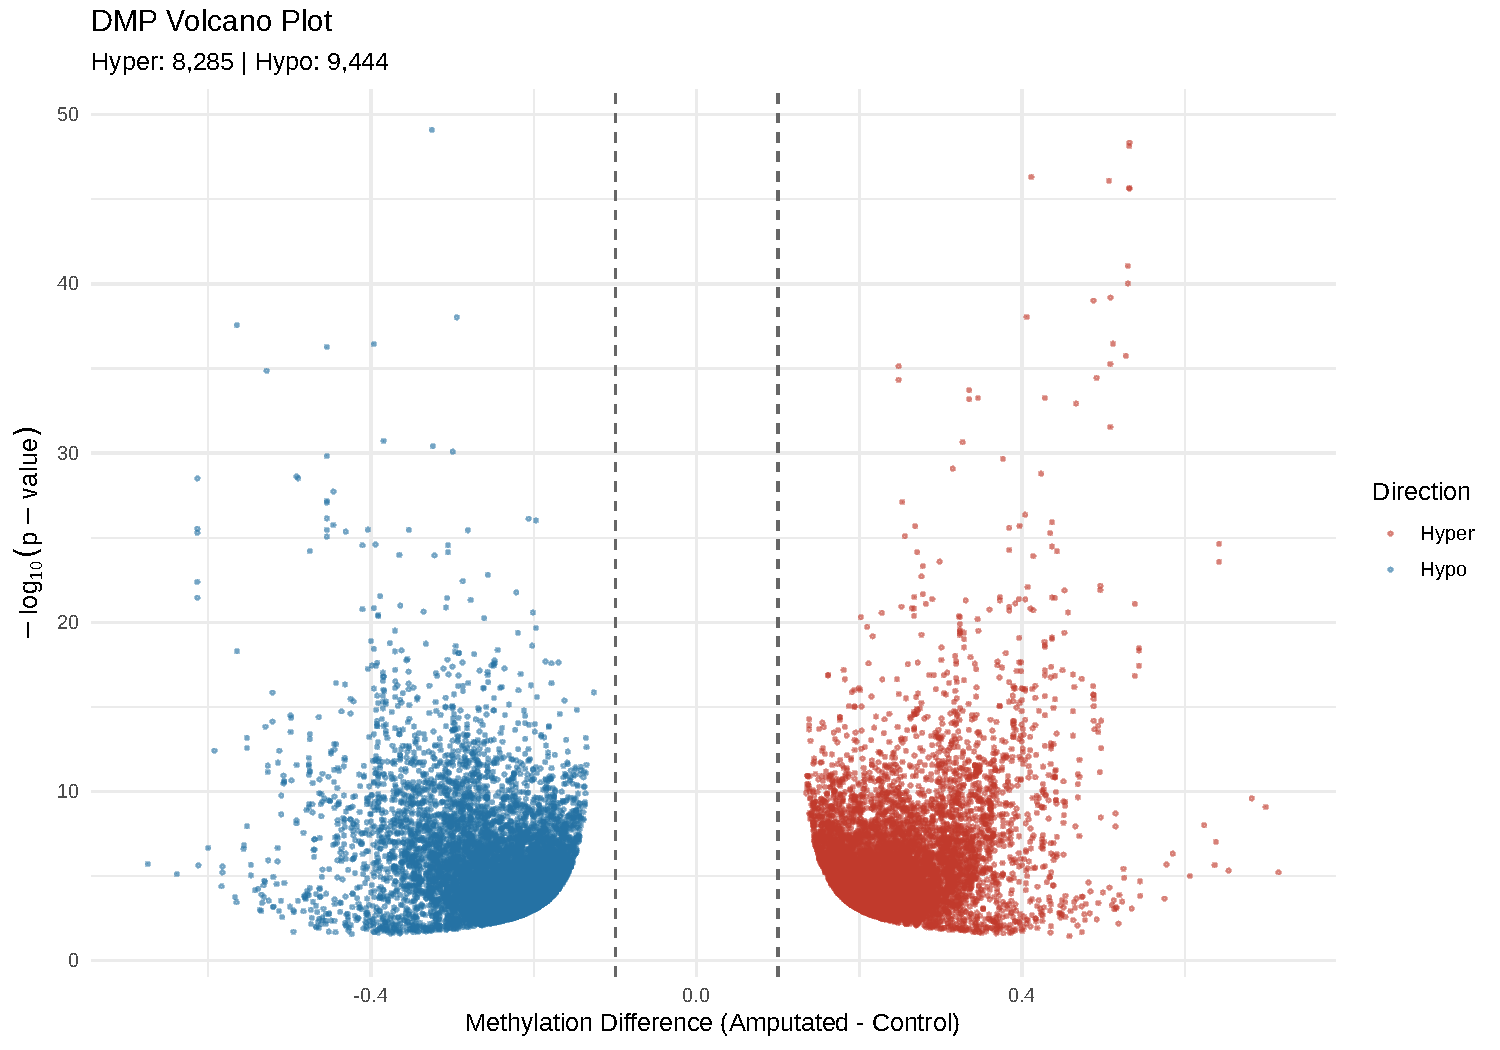
\includegraphics[width=\textwidth]{fig6d_dmp_volcano.pdf}
        \caption{}
    \end{subfigure}
    \hfill
    \begin{subfigure}[b]{0.48\textwidth}
        \centering
        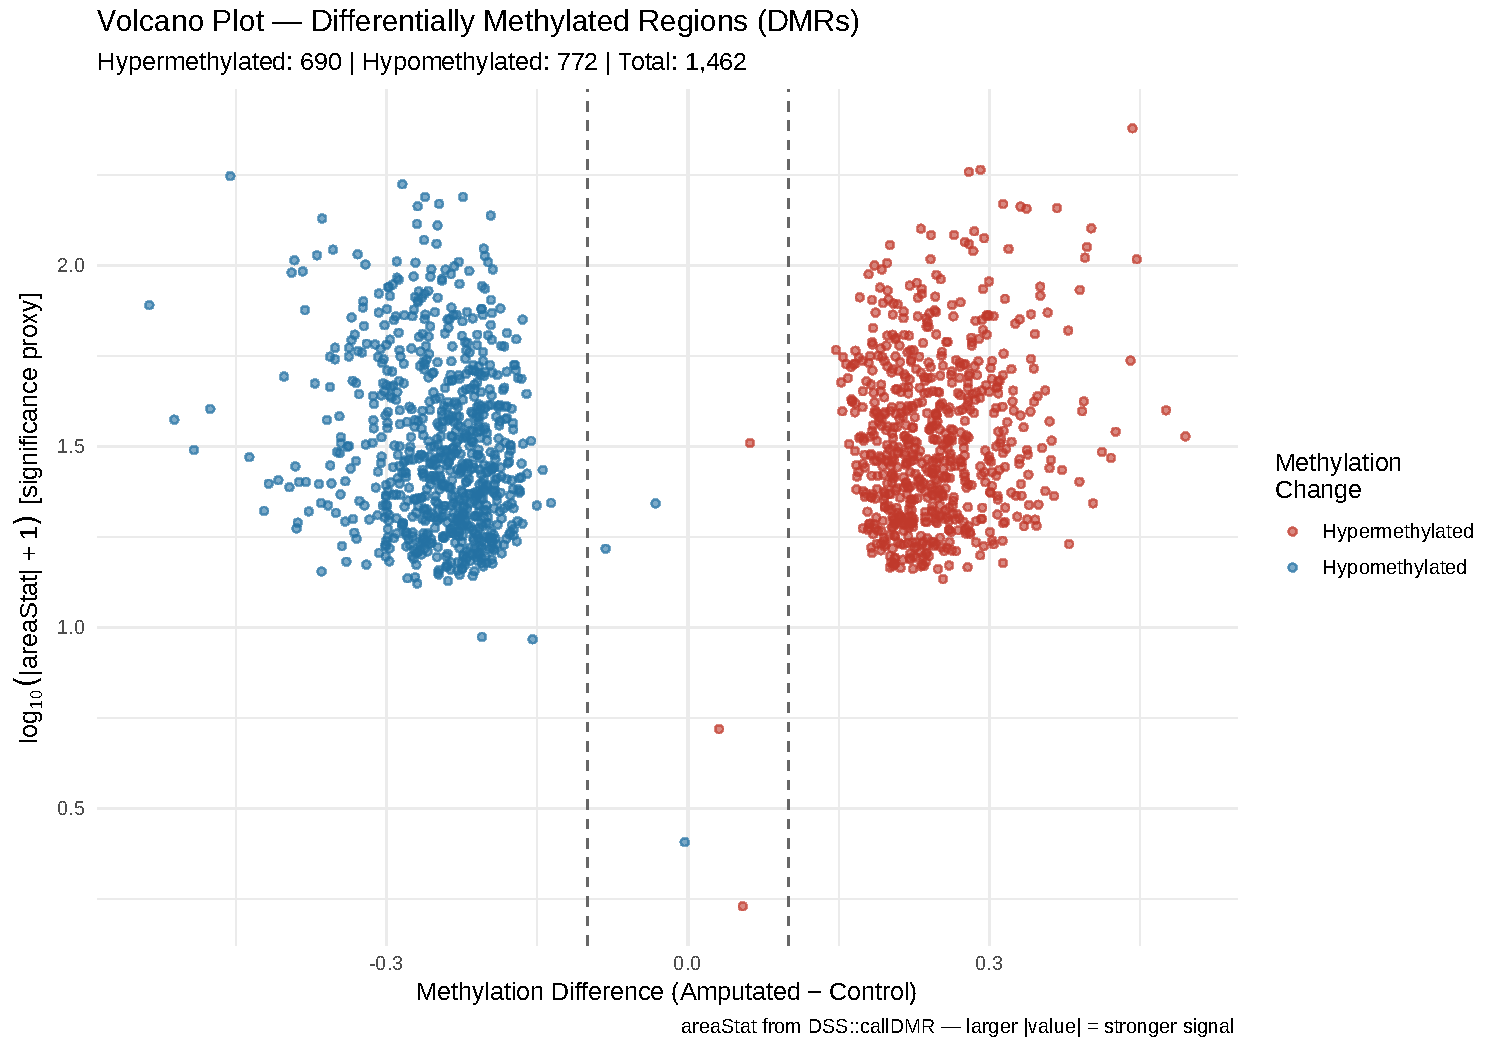
\includegraphics[width=\textwidth]{fig6d3_dmr_volcano.pdf}
        \caption{}
    \end{subfigure}
    \vspace{0.3cm}
    \begin{subfigure}[b]{0.48\textwidth}
        \centering
        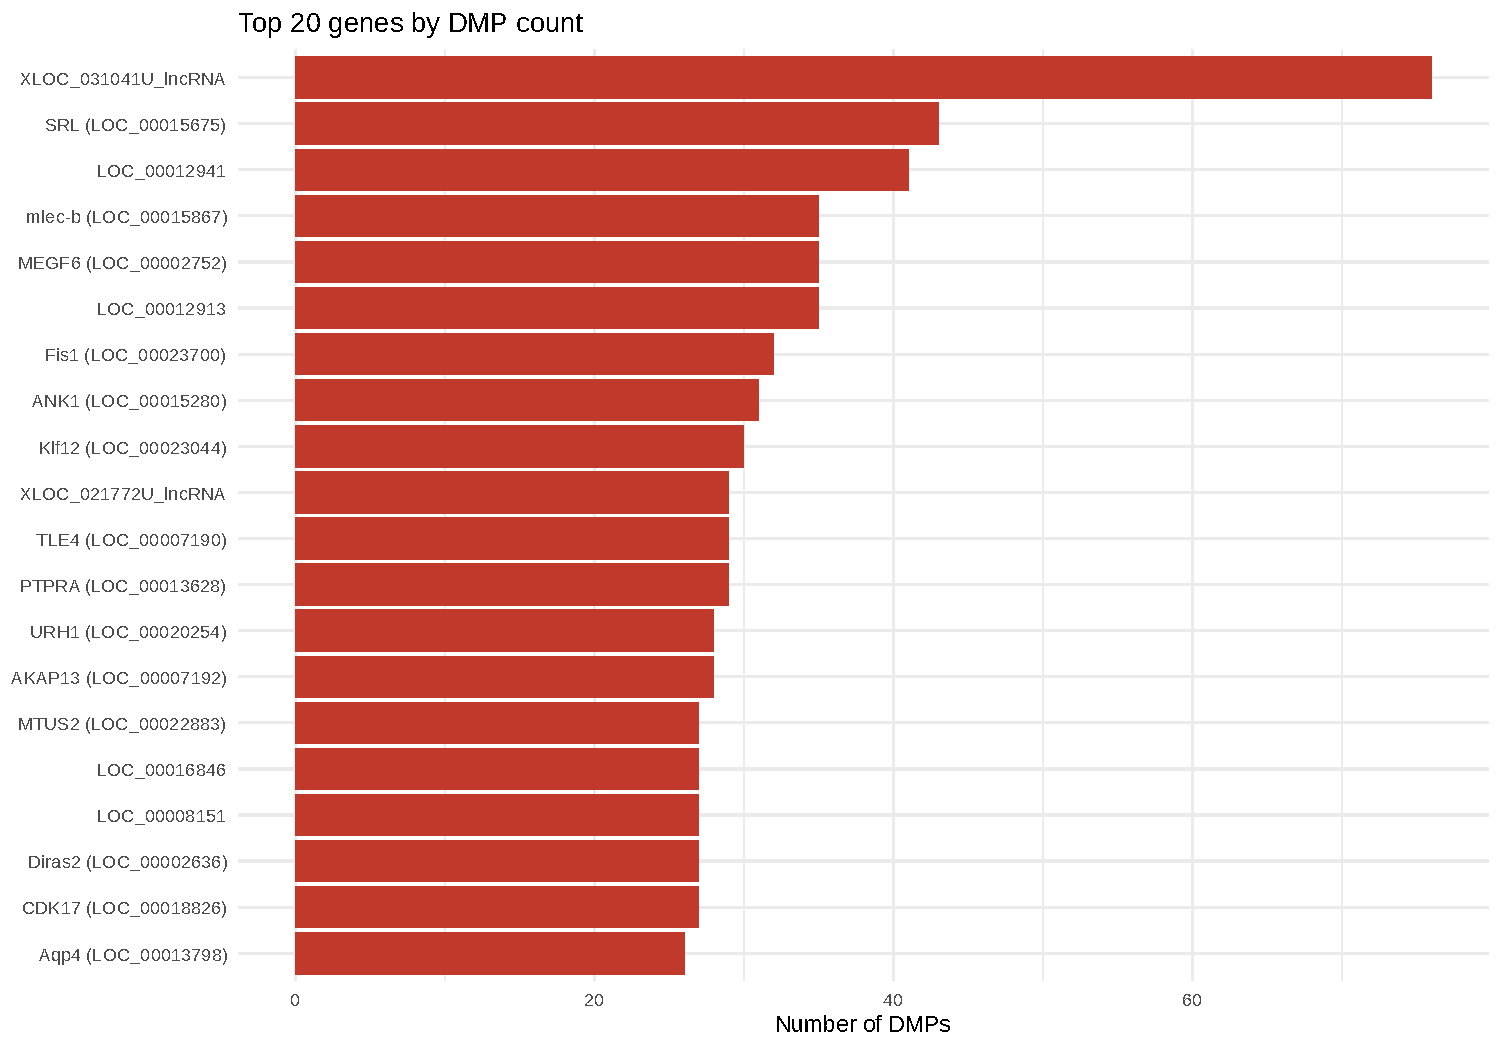
\includegraphics[width=\textwidth]{fig6j_top_genes_dmp.pdf}
        \caption{}
    \end{subfigure}
    \hfill
    \begin{subfigure}[b]{0.48\textwidth}
        \centering
        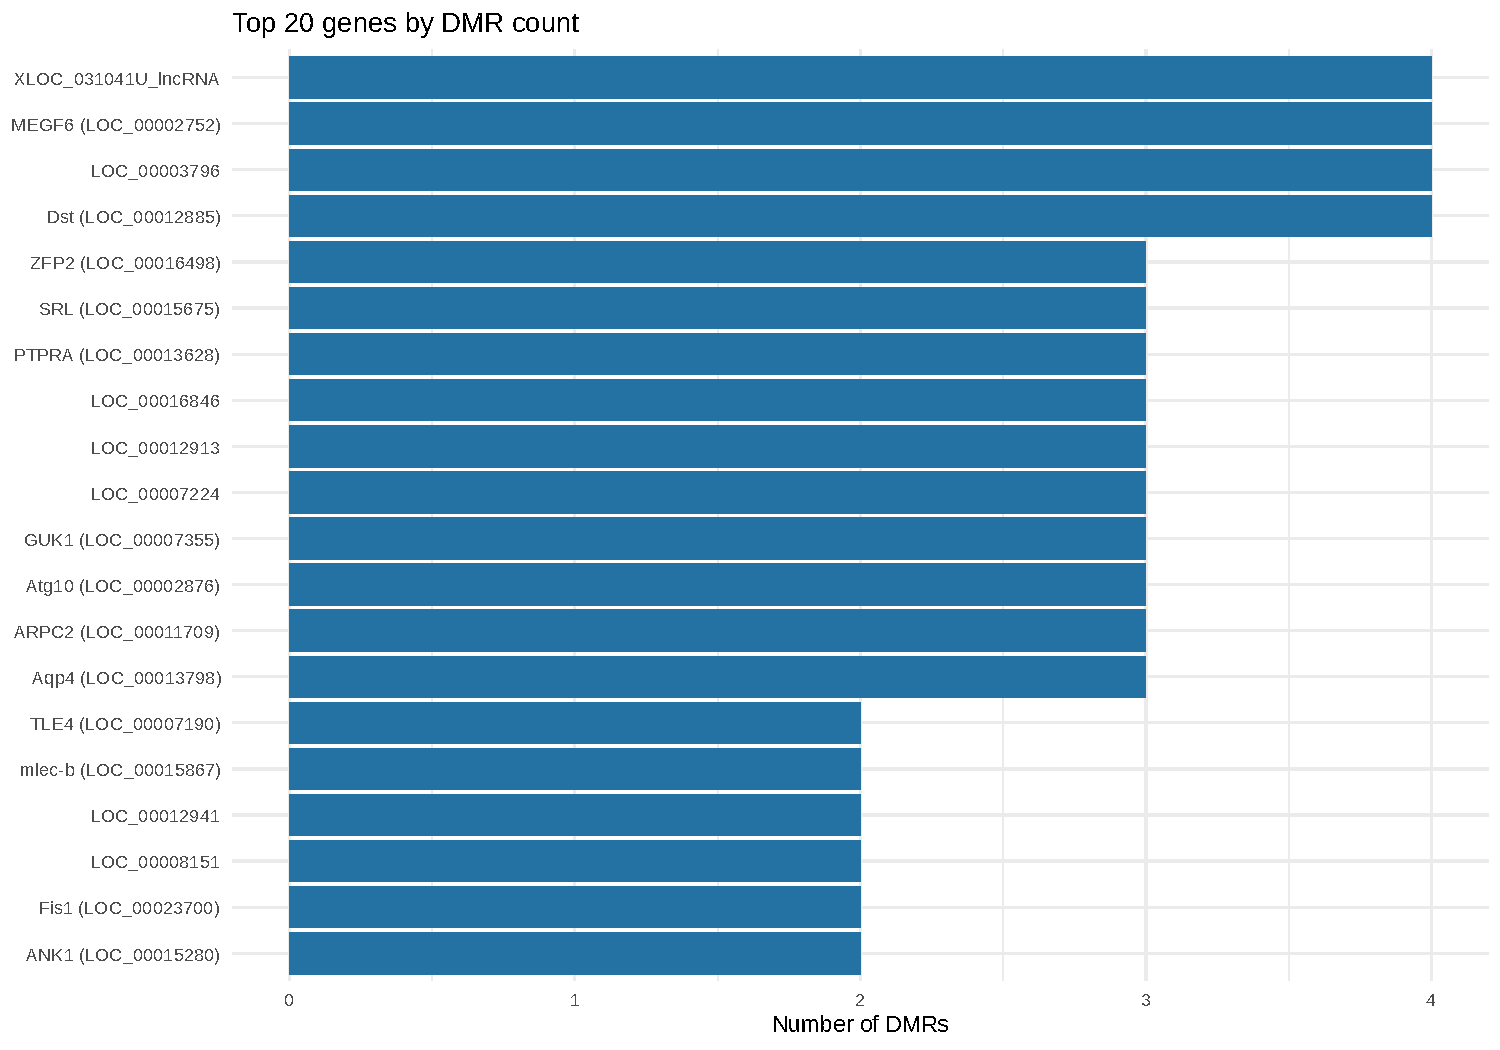
\includegraphics[width=\textwidth]{fig6k_top_genes_dmr.pdf}
        \caption{}
    \end{subfigure}
    \caption{\textbf{Tail amputation reshapes the \textit{D.\ laeve} methylation landscape.}
    (\textbf{A}) Volcano plot of DMPs (17,729 total: 8,285 hyper, 9,444 hypo).
    (\textbf{B}) Volcano plot of DMRs (1,462 total: 690 hyper, 772 hypo).
    (\textbf{C}) Genes ranked by DMP burden.
    (\textbf{D}) Genes ranked by DMR burden.}
    \label{fig:differential}
\end{figure}

\begin{figure}[ht]
    \centering
    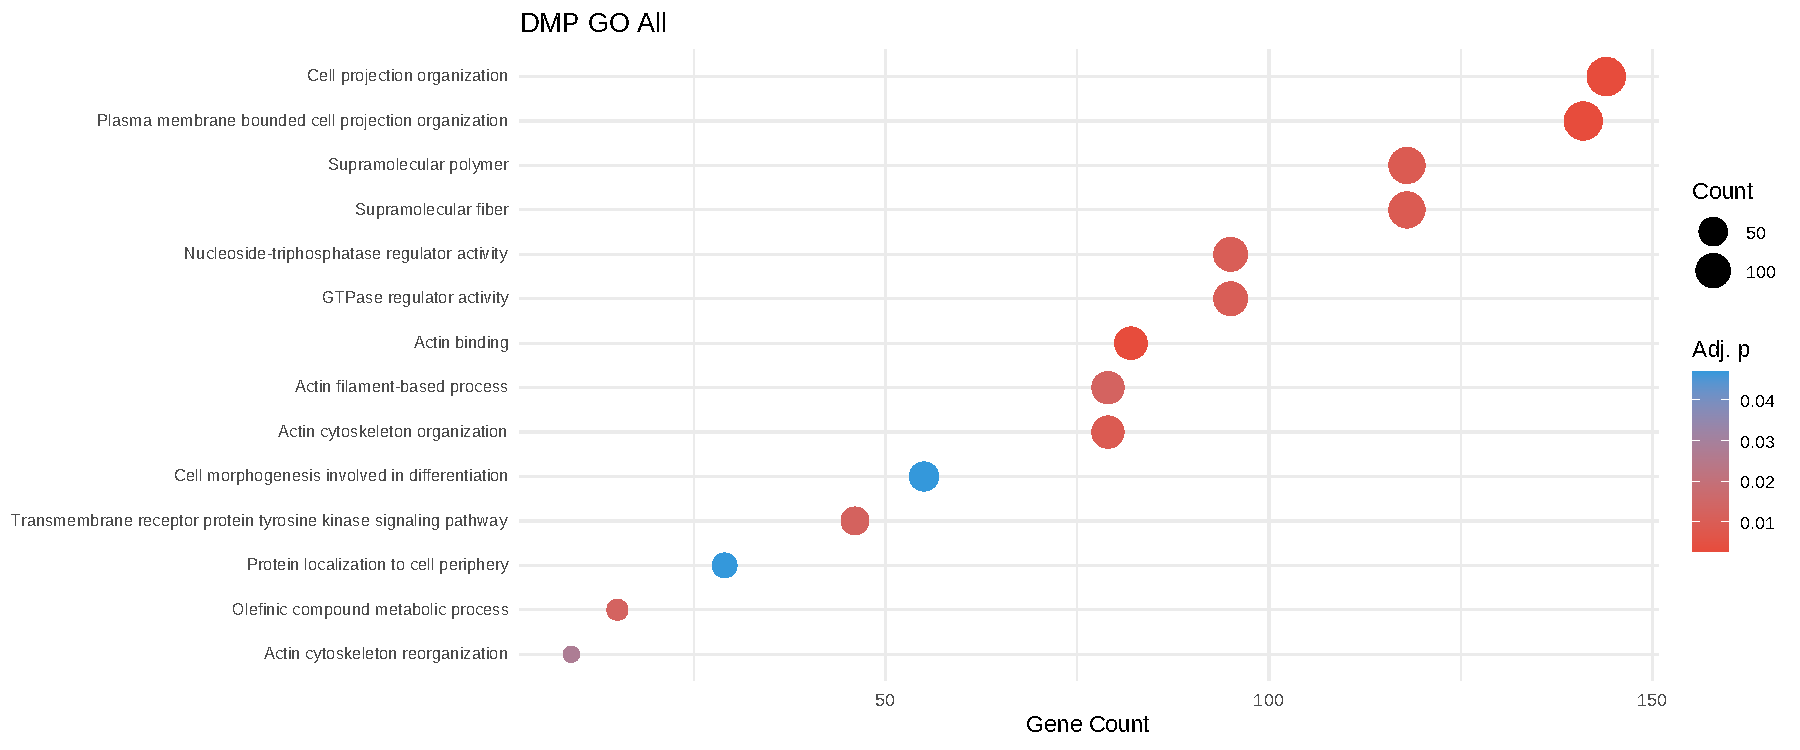
\includegraphics[width=0.90\textwidth]{fig6_dmp_go_all_dotplot.pdf}
    \caption{\textbf{Gene Ontology enrichment of DMP-associated genes.}
    Enrichment analysis of all genes carrying at least one DMP, showing overrepresentation of ciliary architecture, cell projection organization, and morphogenesis terms.}
    \label{fig:go}
\end{figure}


%% =====================================================================
%% FIGURE 7 — METHYLATION-EXPRESSION DECOUPLING
%% =====================================================================

\subsection*{Differential methylation is decoupled from transcriptional changes}

To test whether regeneration-associated methylation changes predict transcriptional changes, we correlated per-gene methylation differences ($\Delta\beta$) with expression changes (log$_2$ fold-change from DESeq2 with apeglm shrinkage) for all genes carrying DMPs or DMRs.

The overall Spearman correlation between DMP-associated methylation change and expression change was $\rho = 0.009$ ($p = 0.55$, $n = 4{,}029$ genes), and the DMR-associated correlation was similarly null ($\rho = -0.021$, $p = 0.43$, $n = 1{,}387$ genes; Fig.~\ref{fig:decoupling}A,~B). This null result held across all genomic regions: promoter, exon, intron, and intergenic DMPs each showed correlations indistinguishable from zero (Fig.~\ref{fig:decoupling}C,~D). Among DMP-carrying genes, only 10.0\% were also differentially expressed (padj $< 0.05$); among DMR-carrying genes, 11.5\% were differentially expressed---rates not substantially elevated above the genome-wide background.

Despite the lack of correlation, 228 genes carried both $\geq$3 DMPs and significant differential expression, forming a concordant gene set enriched for cell adhesion, extracellular matrix remodeling, and cytoskeletal proteins (Fig.~\ref{fig:decoupling}E,~F).

\begin{figure}[ht]
    \centering
    \begin{subfigure}[b]{0.48\textwidth}
        \centering
        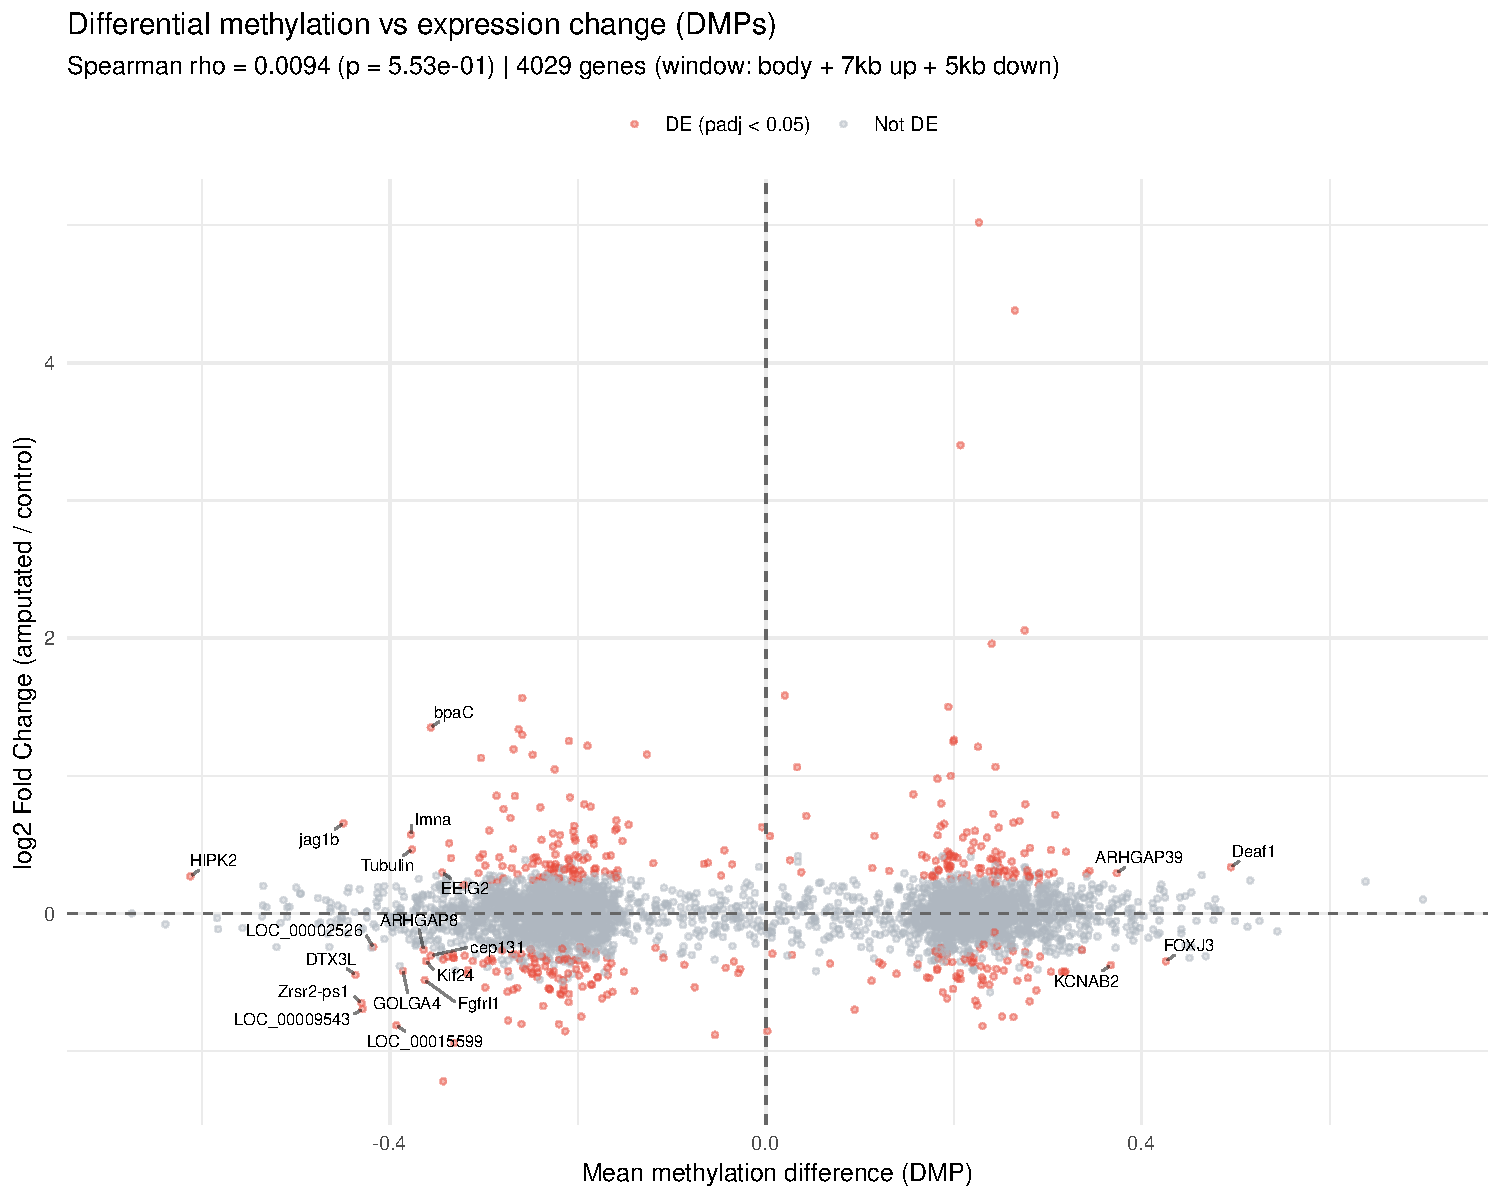
\includegraphics[width=\textwidth]{fig7j_dmp_meth_vs_expression_scatter.pdf}
        \caption{}
    \end{subfigure}
    \hfill
    \begin{subfigure}[b]{0.48\textwidth}
        \centering
        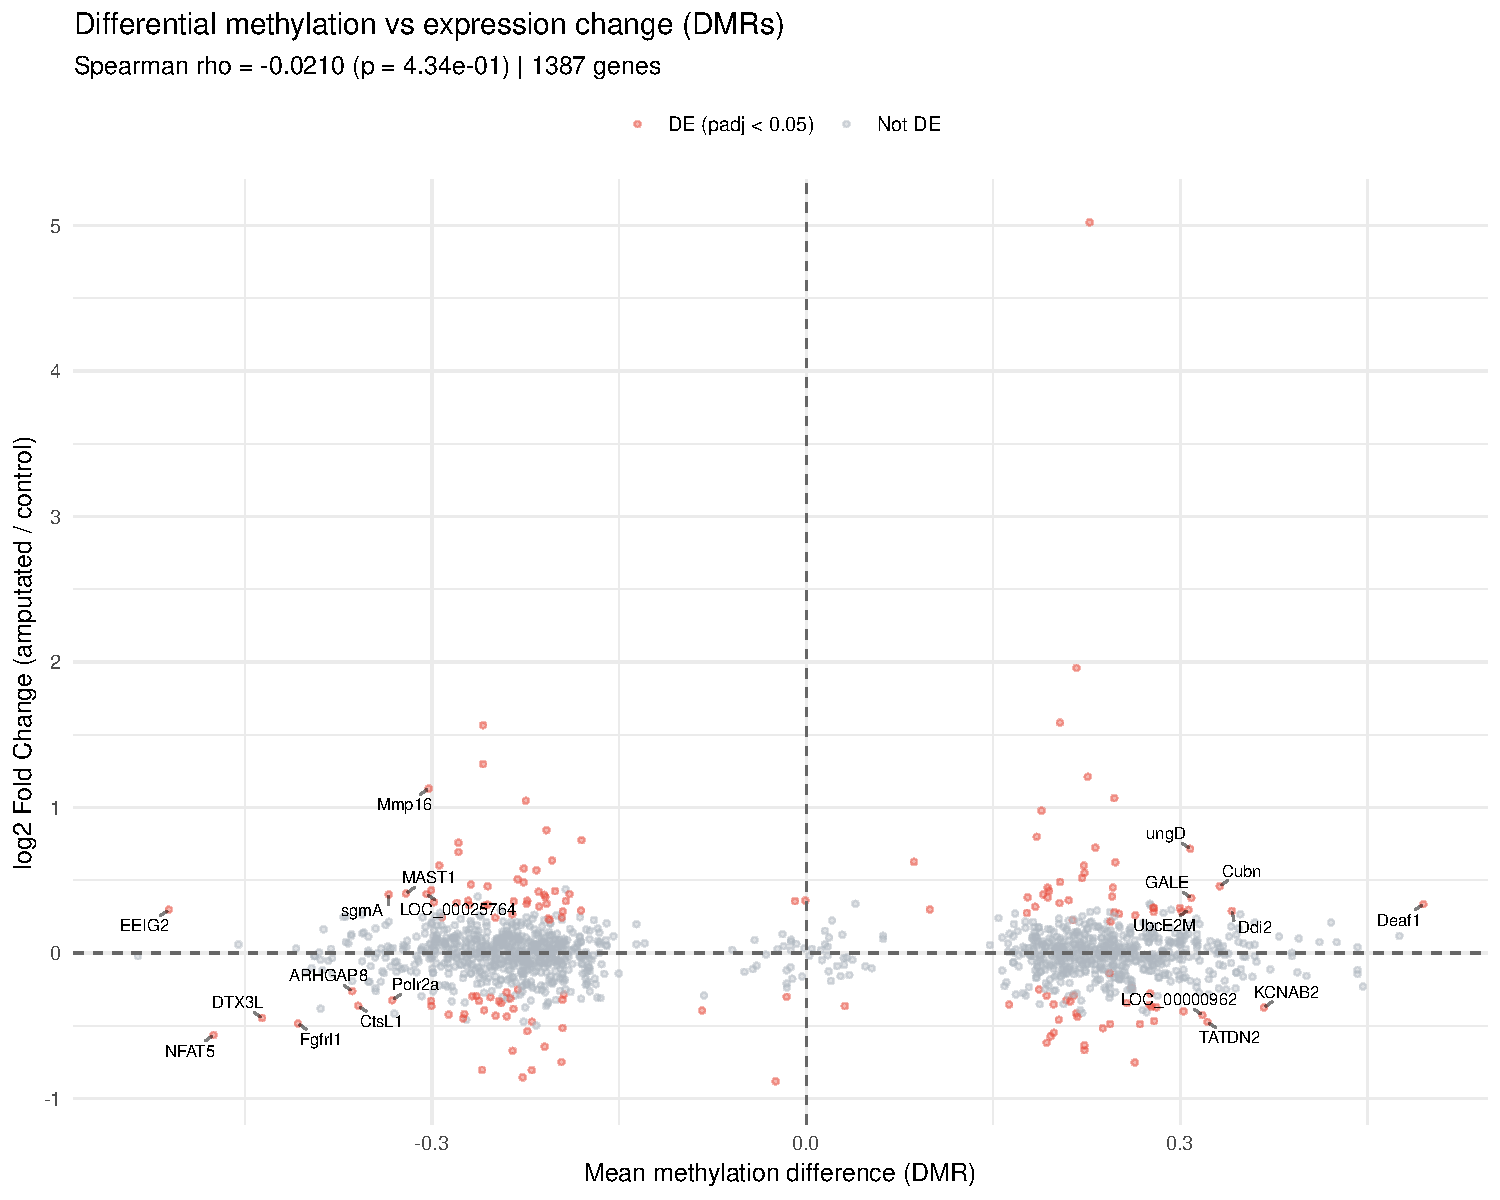
\includegraphics[width=\textwidth]{fig7k_dmr_meth_vs_expression_scatter.pdf}
        \caption{}
    \end{subfigure}
    \vspace{0.3cm}
    \begin{subfigure}[b]{0.48\textwidth}
        \centering
        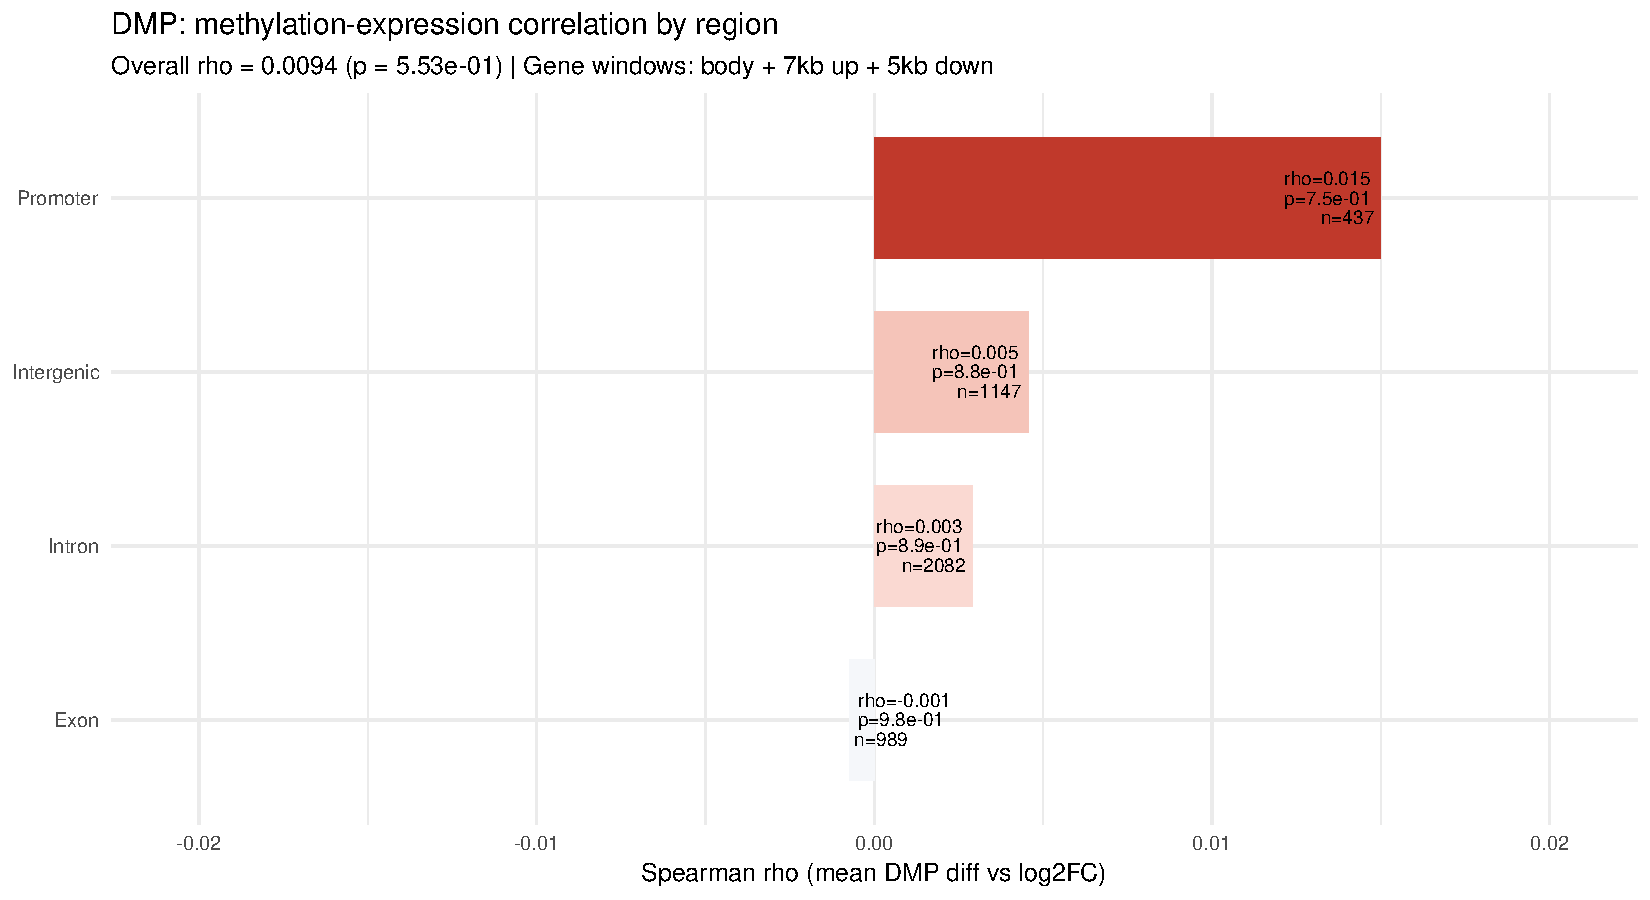
\includegraphics[width=\textwidth]{fig7a_dmp_correlation_by_region.pdf}
        \caption{}
    \end{subfigure}
    \hfill
    \begin{subfigure}[b]{0.48\textwidth}
        \centering
        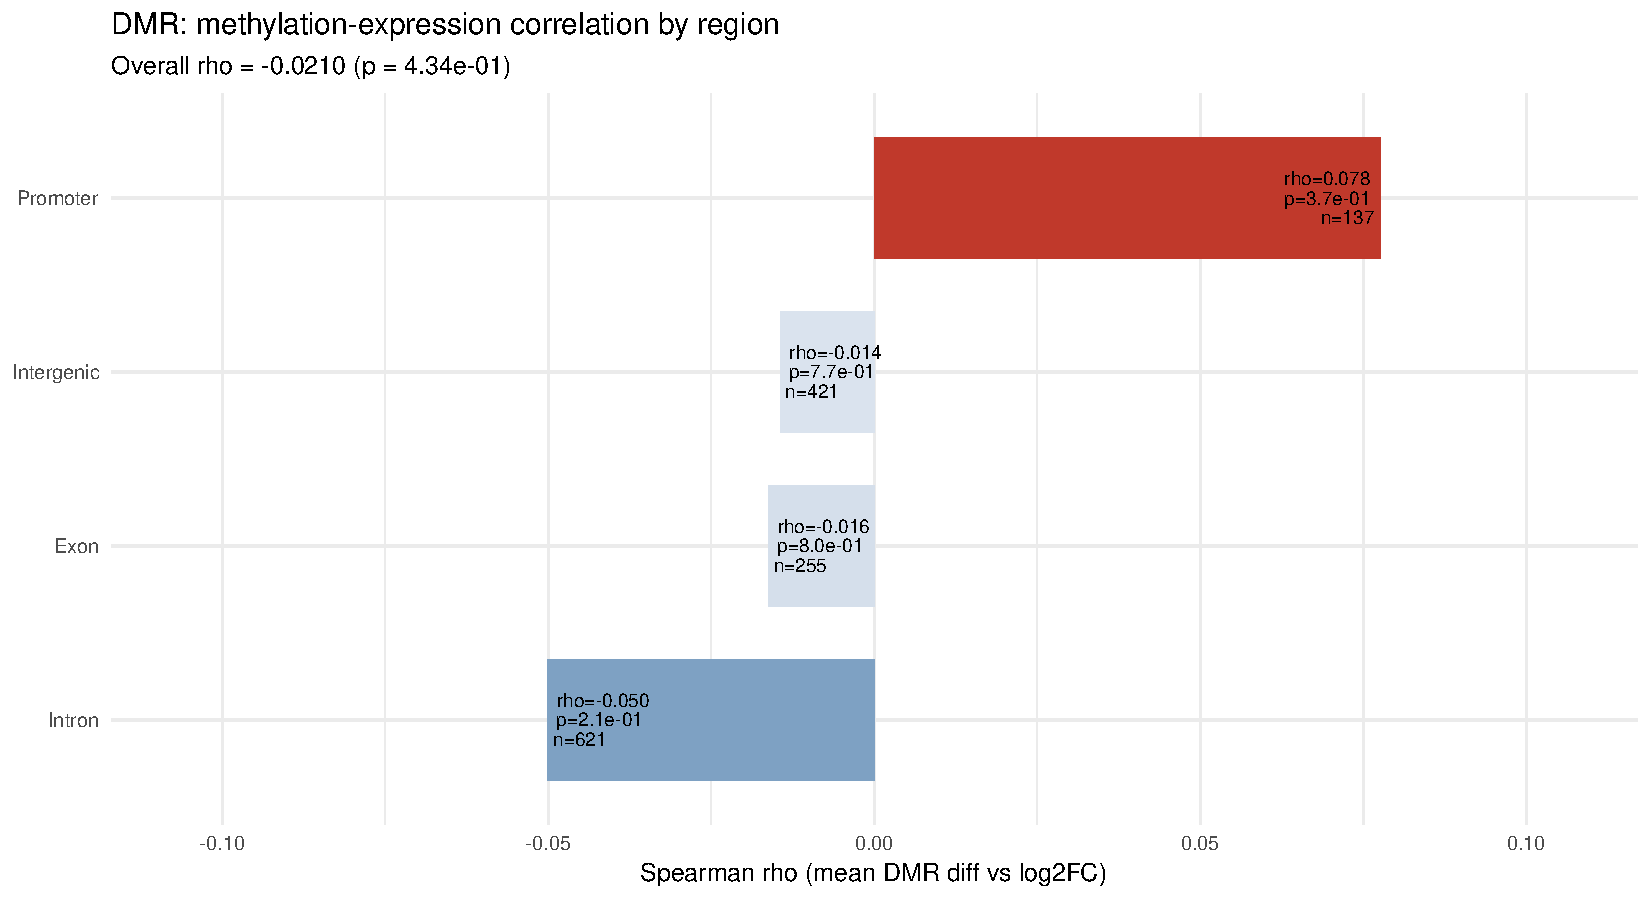
\includegraphics[width=\textwidth]{fig7b_dmr_correlation_by_region.pdf}
        \caption{}
    \end{subfigure}
    \caption{\textbf{Differential methylation is decoupled from transcriptional changes.}
    (\textbf{A}) DMP-associated methylation change vs.\ expression change (Spearman $\rho = 0.009$, $p = 0.55$).
    (\textbf{B}) DMR-associated methylation change vs.\ expression change ($\rho = -0.021$, $p = 0.43$).
    (\textbf{C},~\textbf{D}) Spearman correlation by genomic region for DMPs and DMRs; all regions show $\rho \approx 0$.}
    \label{fig:decoupling}
\end{figure}

\begin{figure}[ht]
    \centering
    \begin{subfigure}[b]{0.48\textwidth}
        \centering
        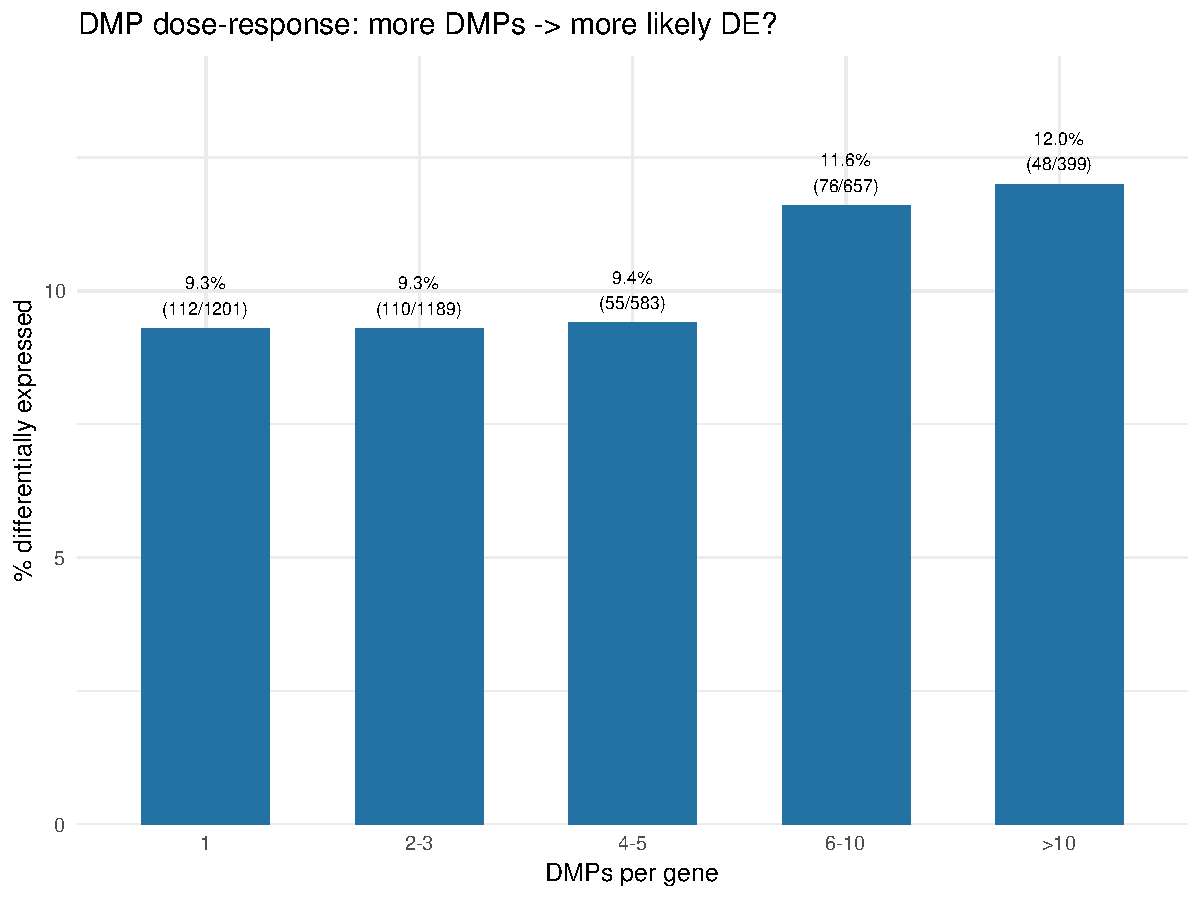
\includegraphics[width=\textwidth]{fig7e_dmp_dose_response.pdf}
        \caption{}
    \end{subfigure}
    \hfill
    \begin{subfigure}[b]{0.48\textwidth}
        \centering
        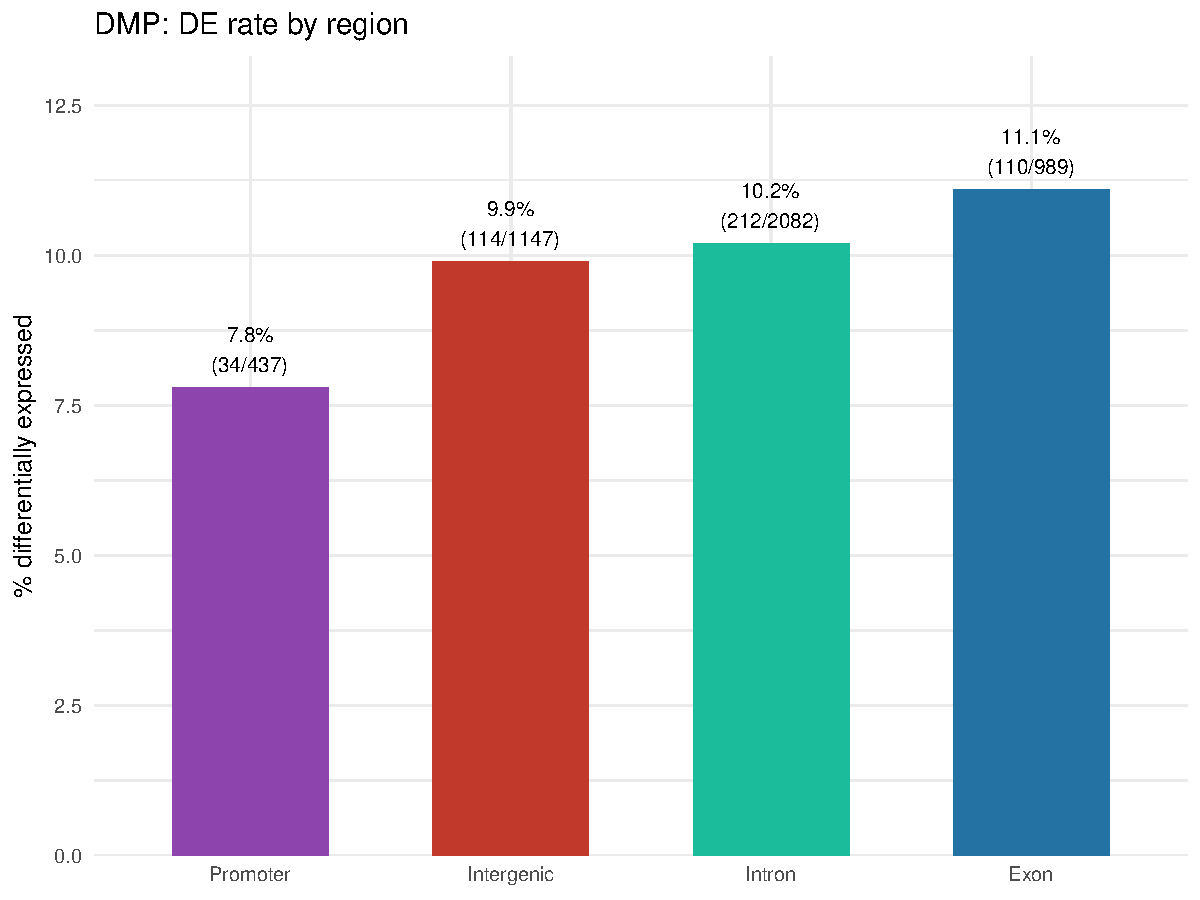
\includegraphics[width=\textwidth]{fig7c_dmp_de_rate_by_region.pdf}
        \caption{}
    \end{subfigure}
    \caption{\textbf{DMP burden does not predict differential expression.}
    (\textbf{A}) Dose--response: DMP burden bins vs.\ differential expression rate.
    (\textbf{B}) DE rate among DMP-carrying genes by genomic region.}
    \label{fig:doseresp}
\end{figure}


%% =====================================================================
%% FIGURE 8 — WGCNA CO-EXPRESSION MODULES
%% =====================================================================

\subsection*{Differentially methylated genes are enriched in tissue-specific co-expression modules}

The lack of a global correlation between methylation change and expression change at the individual-gene level does not preclude the possibility that methylation changes are concentrated in specific biological programs. To test this, we performed weighted gene co-expression network analysis (WGCNA) using RNA-seq data from six tissues---tail (control and amputated), eye (control and amputated), body wall (control, irradiated, and fungicide-exposed), head, juvenile, and ovotestis---and asked whether DMP-carrying genes were non-randomly distributed across the resulting co-expression modules.

WGCNA identified a set of co-expression modules using a soft-thresholding power of 12, each containing genes with correlated expression patterns across tissues (Fig.~\ref{fig:wgcna}A,~B). Module--trait correlation analysis, using tissue$\times$condition interaction terms to avoid conflating control and amputated samples within the same tissue, revealed that specific modules were strongly associated with tissue identity, with distinct modules enriched for genes characteristic of the ovotestis, the eye, and the body wall (Fig.~\ref{fig:wgcna}C). When we computed the DMP burden per module, we found that DMP burden was not uniformly distributed (Fig.~\ref{fig:wgcna}D). Fisher's exact tests confirmed that several modules were significantly enriched for DMP-carrying genes beyond what would be expected by chance (Fig.~\ref{fig:wgcna}E).

The modules most strongly enriched for DMPs included one associated with the ovotestis transcriptome and another enriched for genes involved in morphogenesis, ciliary assembly, and cytoskeletal organization (Fig.~\ref{fig:wgcna}F). The enrichment of DMPs in tissue-specific modules, particularly the ovotestis module, is consistent with the interpretation that methylation changes during blastema formation may reflect shifts in cell-type composition rather than \textit{cis}-regulatory changes within individual cell types.

\begin{figure}[ht]
    \centering

    \begin{subfigure}[b]{0.48\textwidth}
        \centering
        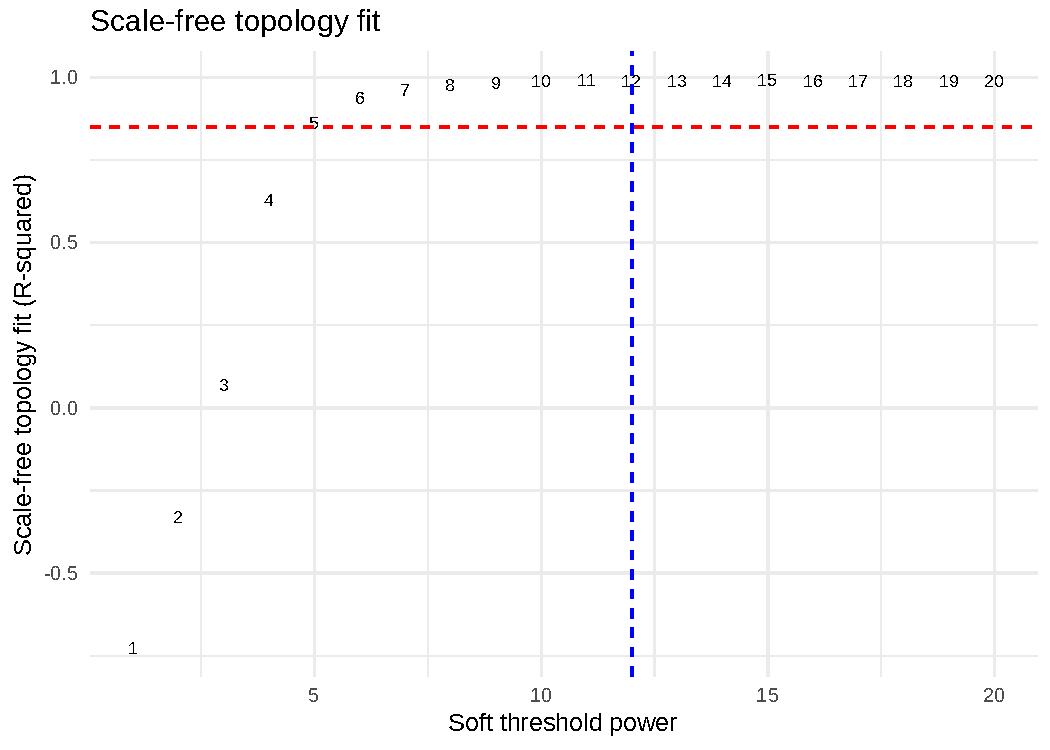
\includegraphics[width=\textwidth]{fig8b_soft_threshold.pdf}
        \caption{}
    \end{subfigure}
    \hfill
    \begin{subfigure}[b]{0.48\textwidth}
        \centering
        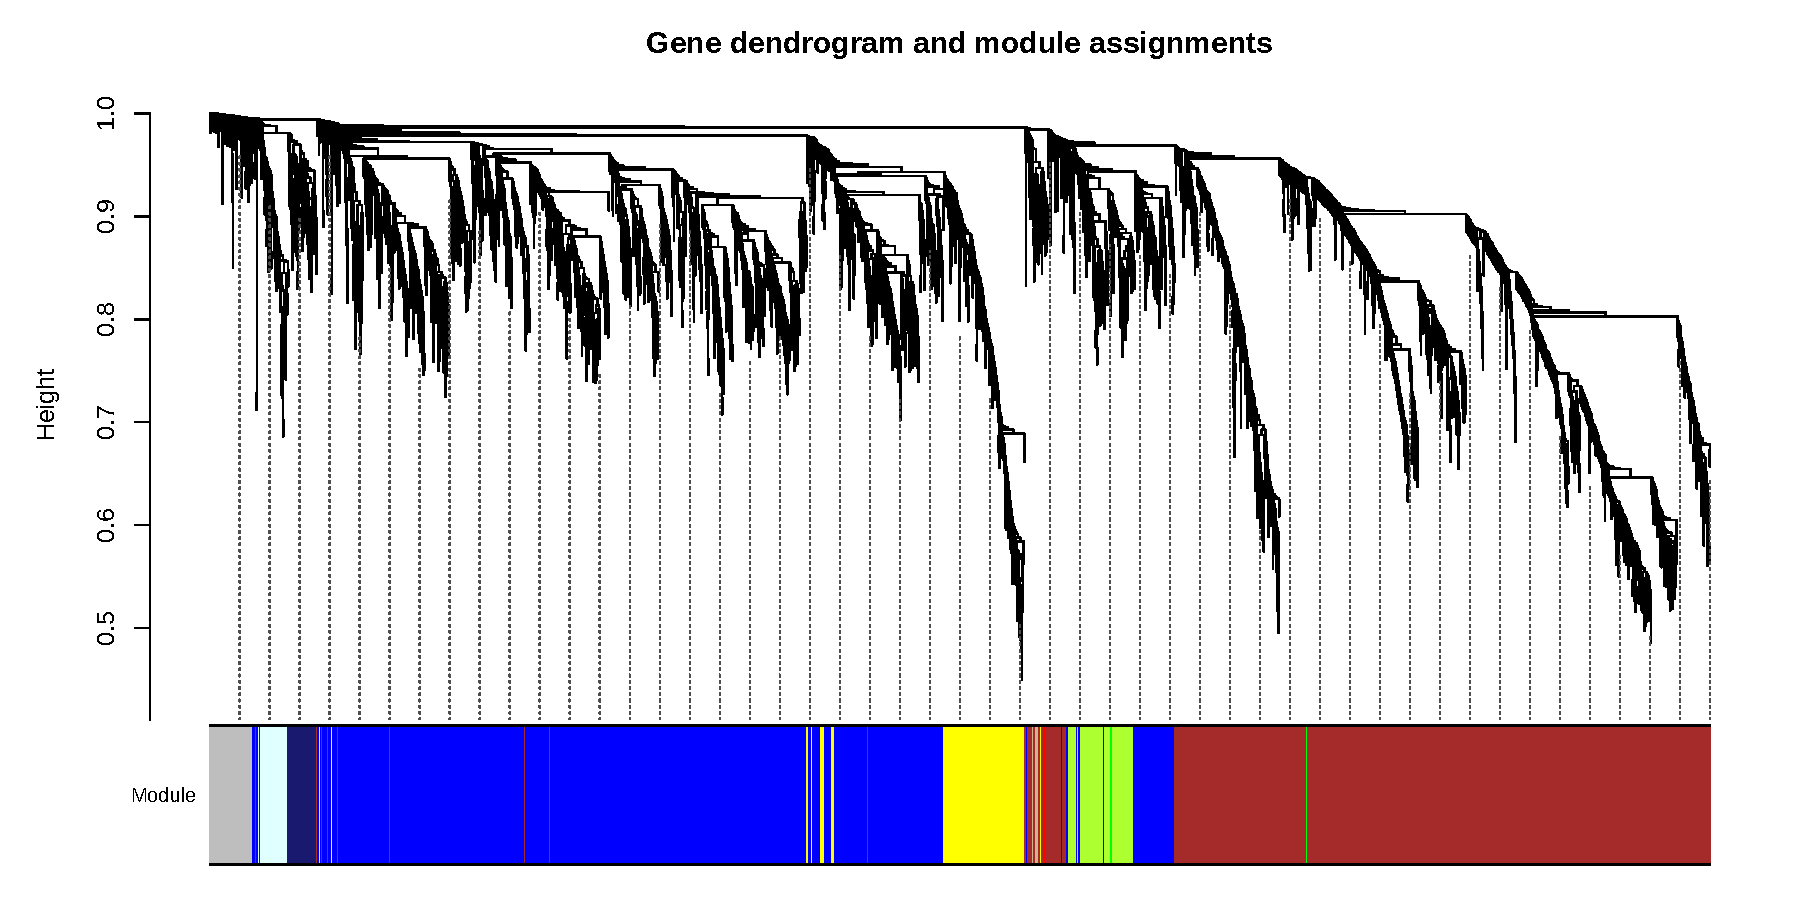
\includegraphics[width=\textwidth]{fig8c_module_dendrogram.pdf}
        \caption{}
    \end{subfigure}

    \vspace{0.5cm}

    \begin{subfigure}[b]{0.48\textwidth}
        \centering
        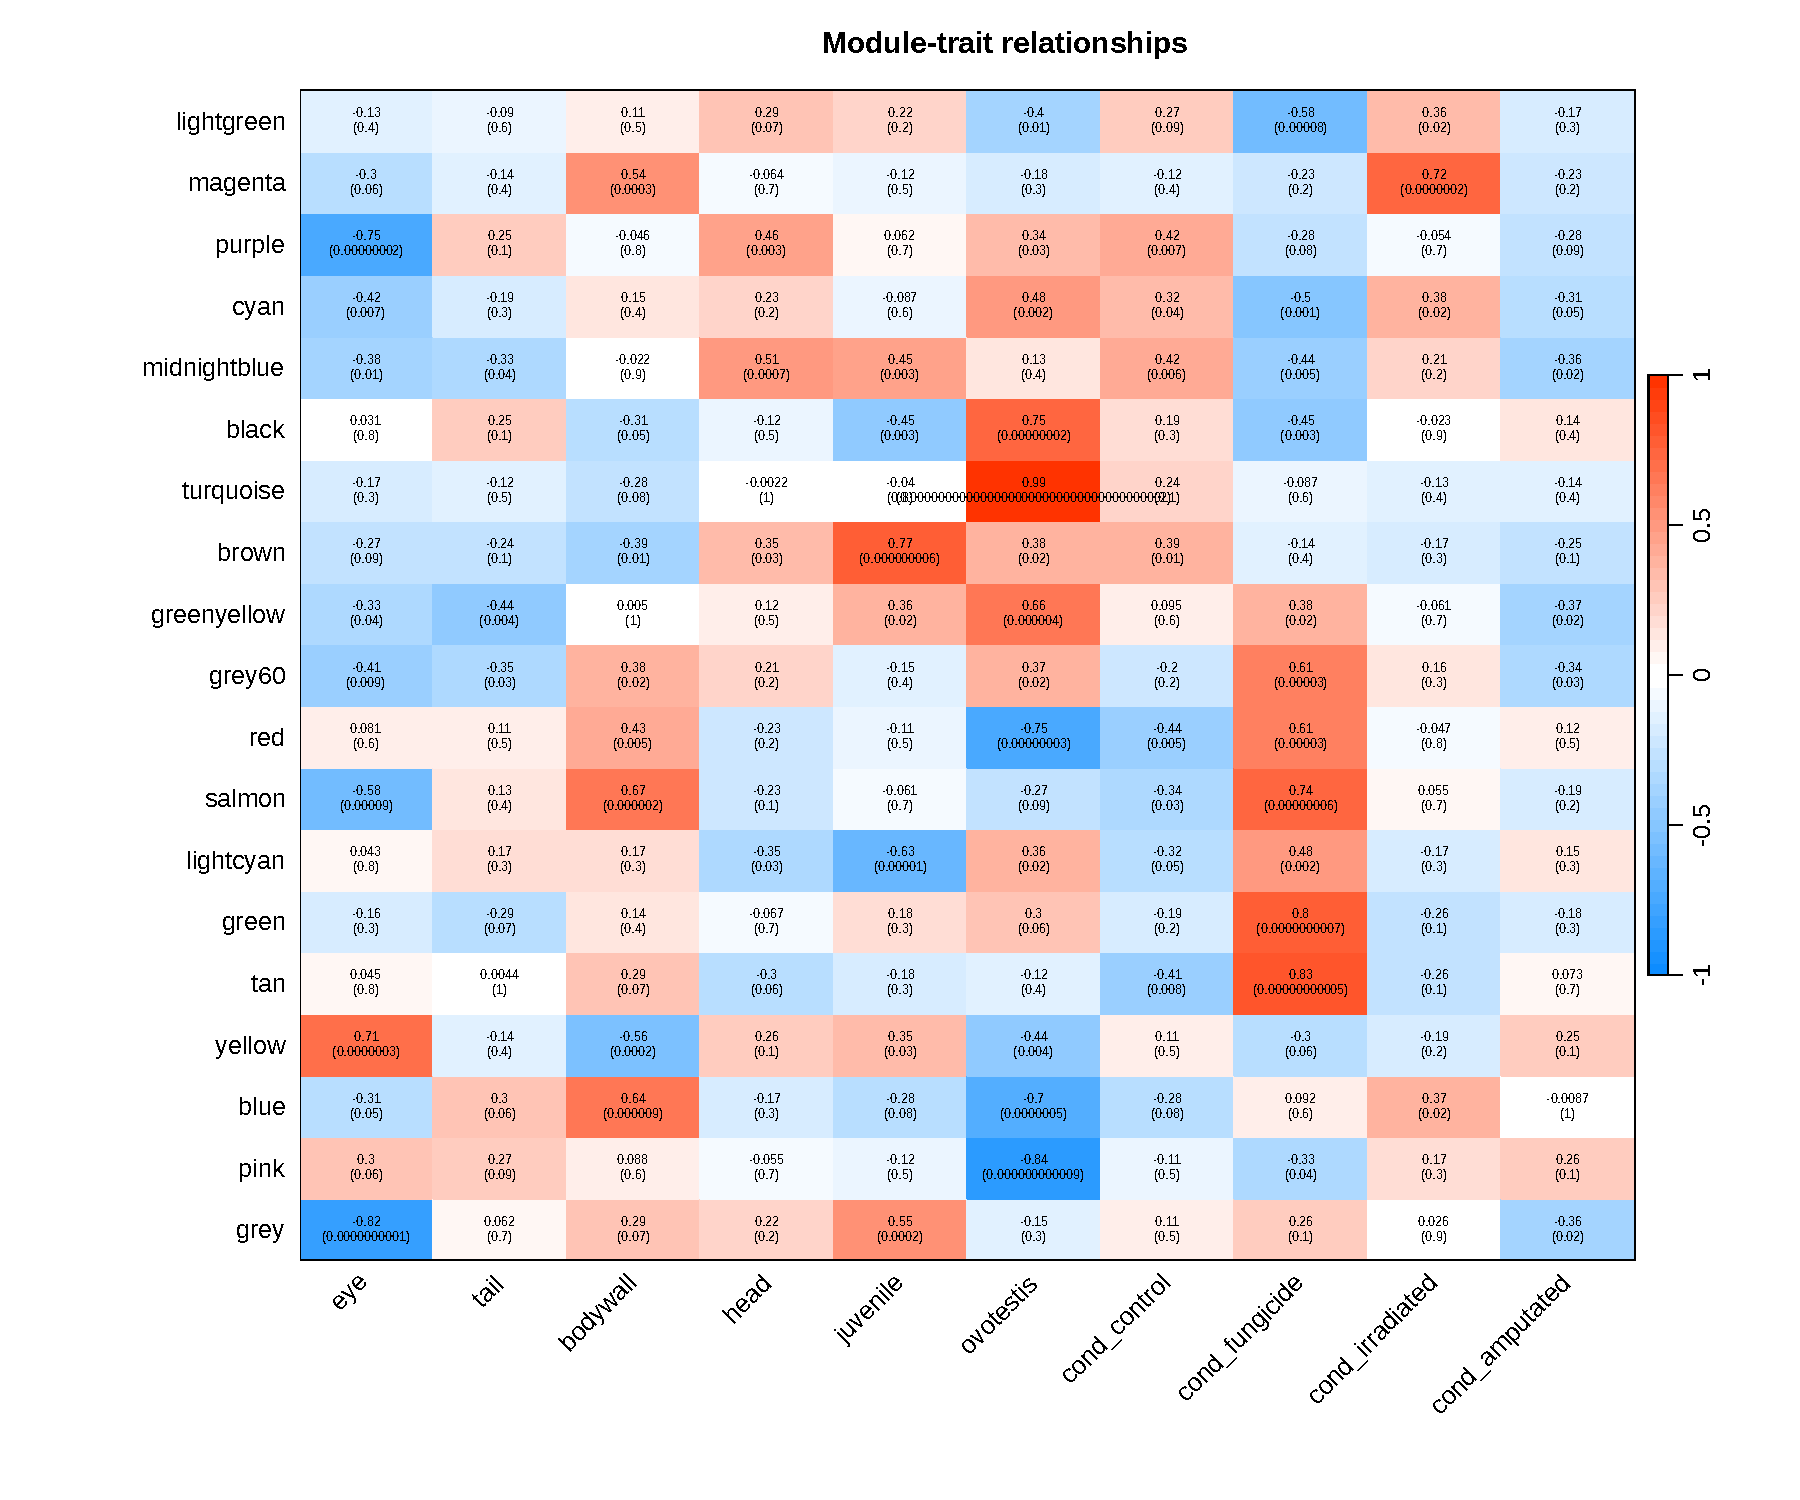
\includegraphics[width=\textwidth]{fig8d_module_trait_heatmap.pdf}
        \caption{}
    \end{subfigure}
    \hfill
    \begin{subfigure}[b]{0.48\textwidth}
        \centering
        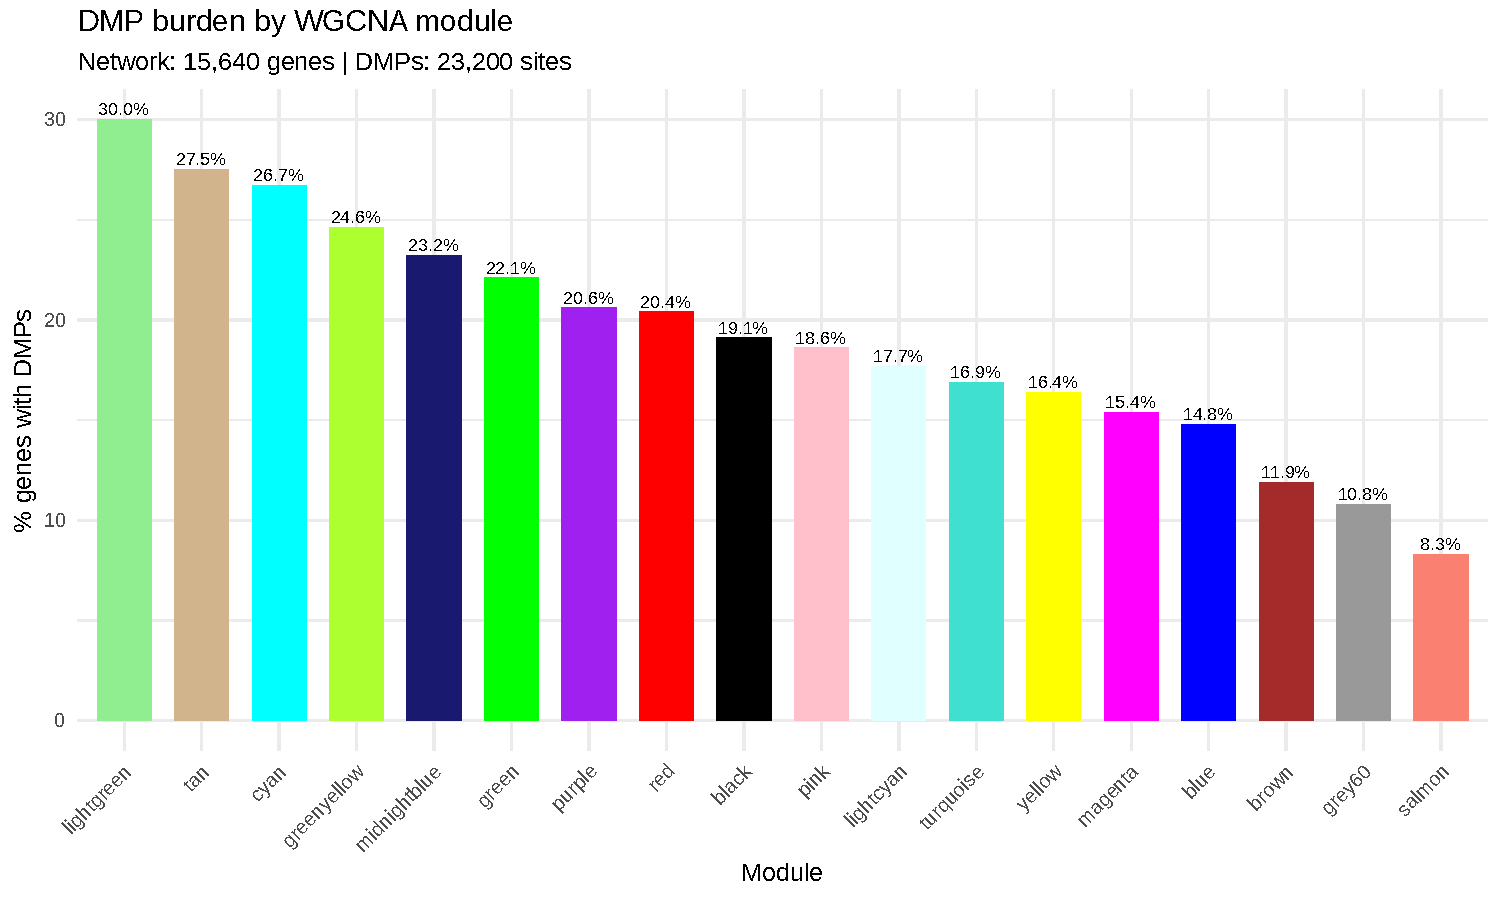
\includegraphics[width=\textwidth]{fig8f_module_dmp_burden.pdf}
        \caption{}
    \end{subfigure}

    \vspace{0.5cm}

    \begin{subfigure}[b]{0.48\textwidth}
        \centering
        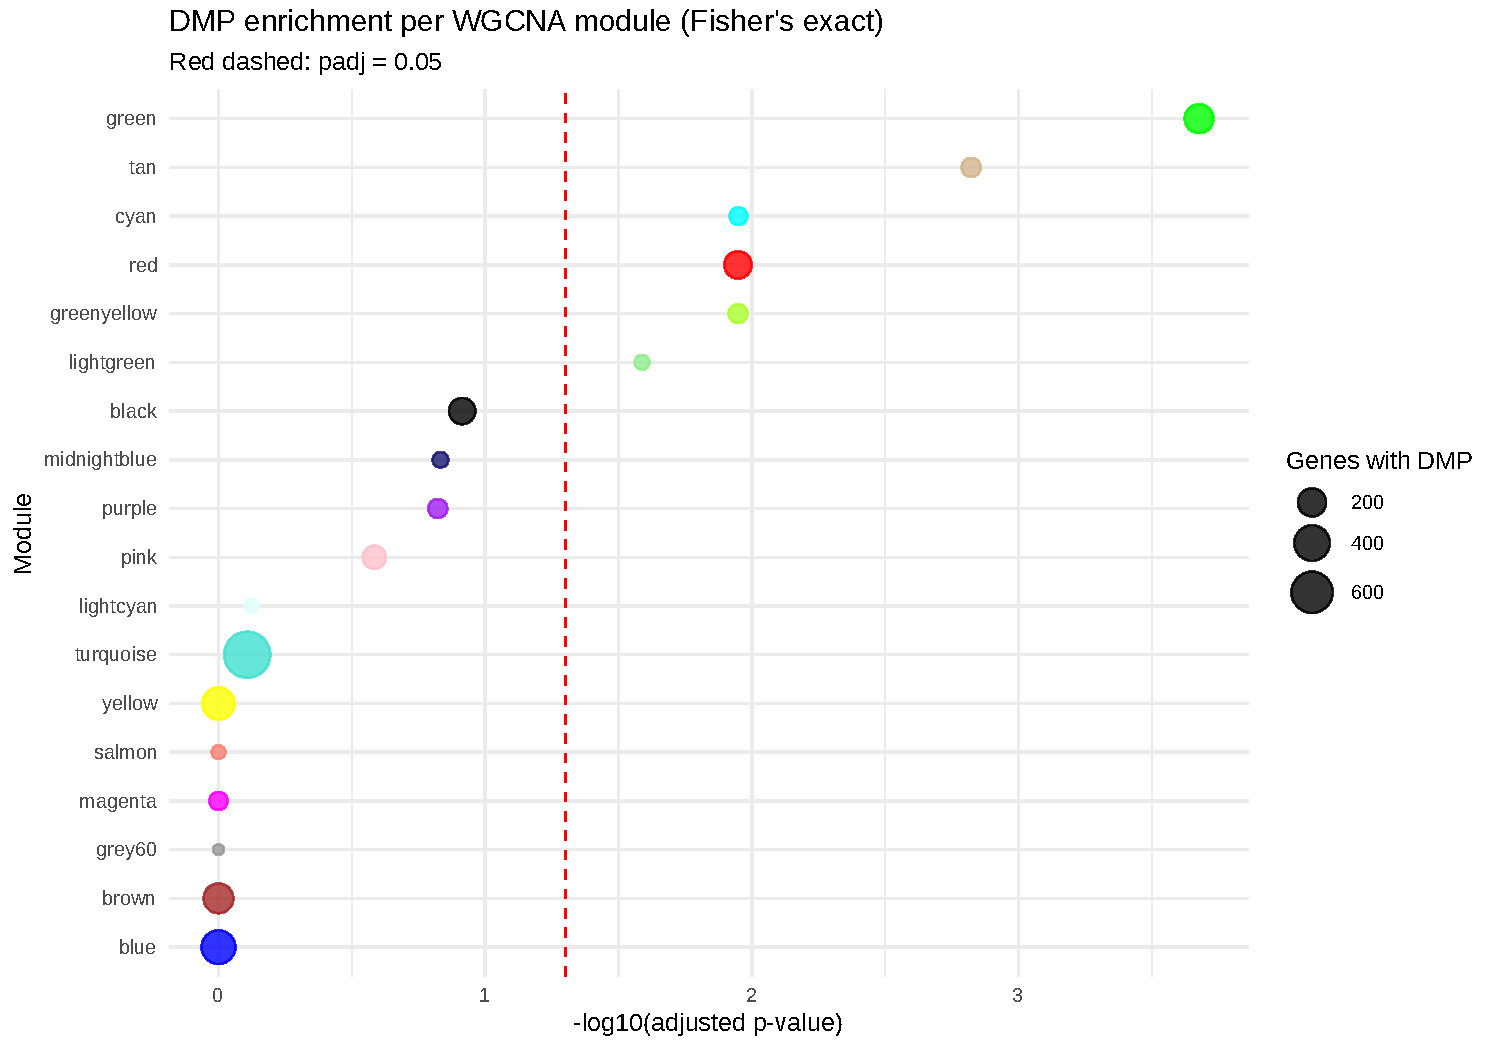
\includegraphics[width=\textwidth]{fig8g_fisher_dmp_enrichment.pdf}
        \caption{}
    \end{subfigure}
    \hfill
    \begin{subfigure}[b]{0.48\textwidth}
        \centering
        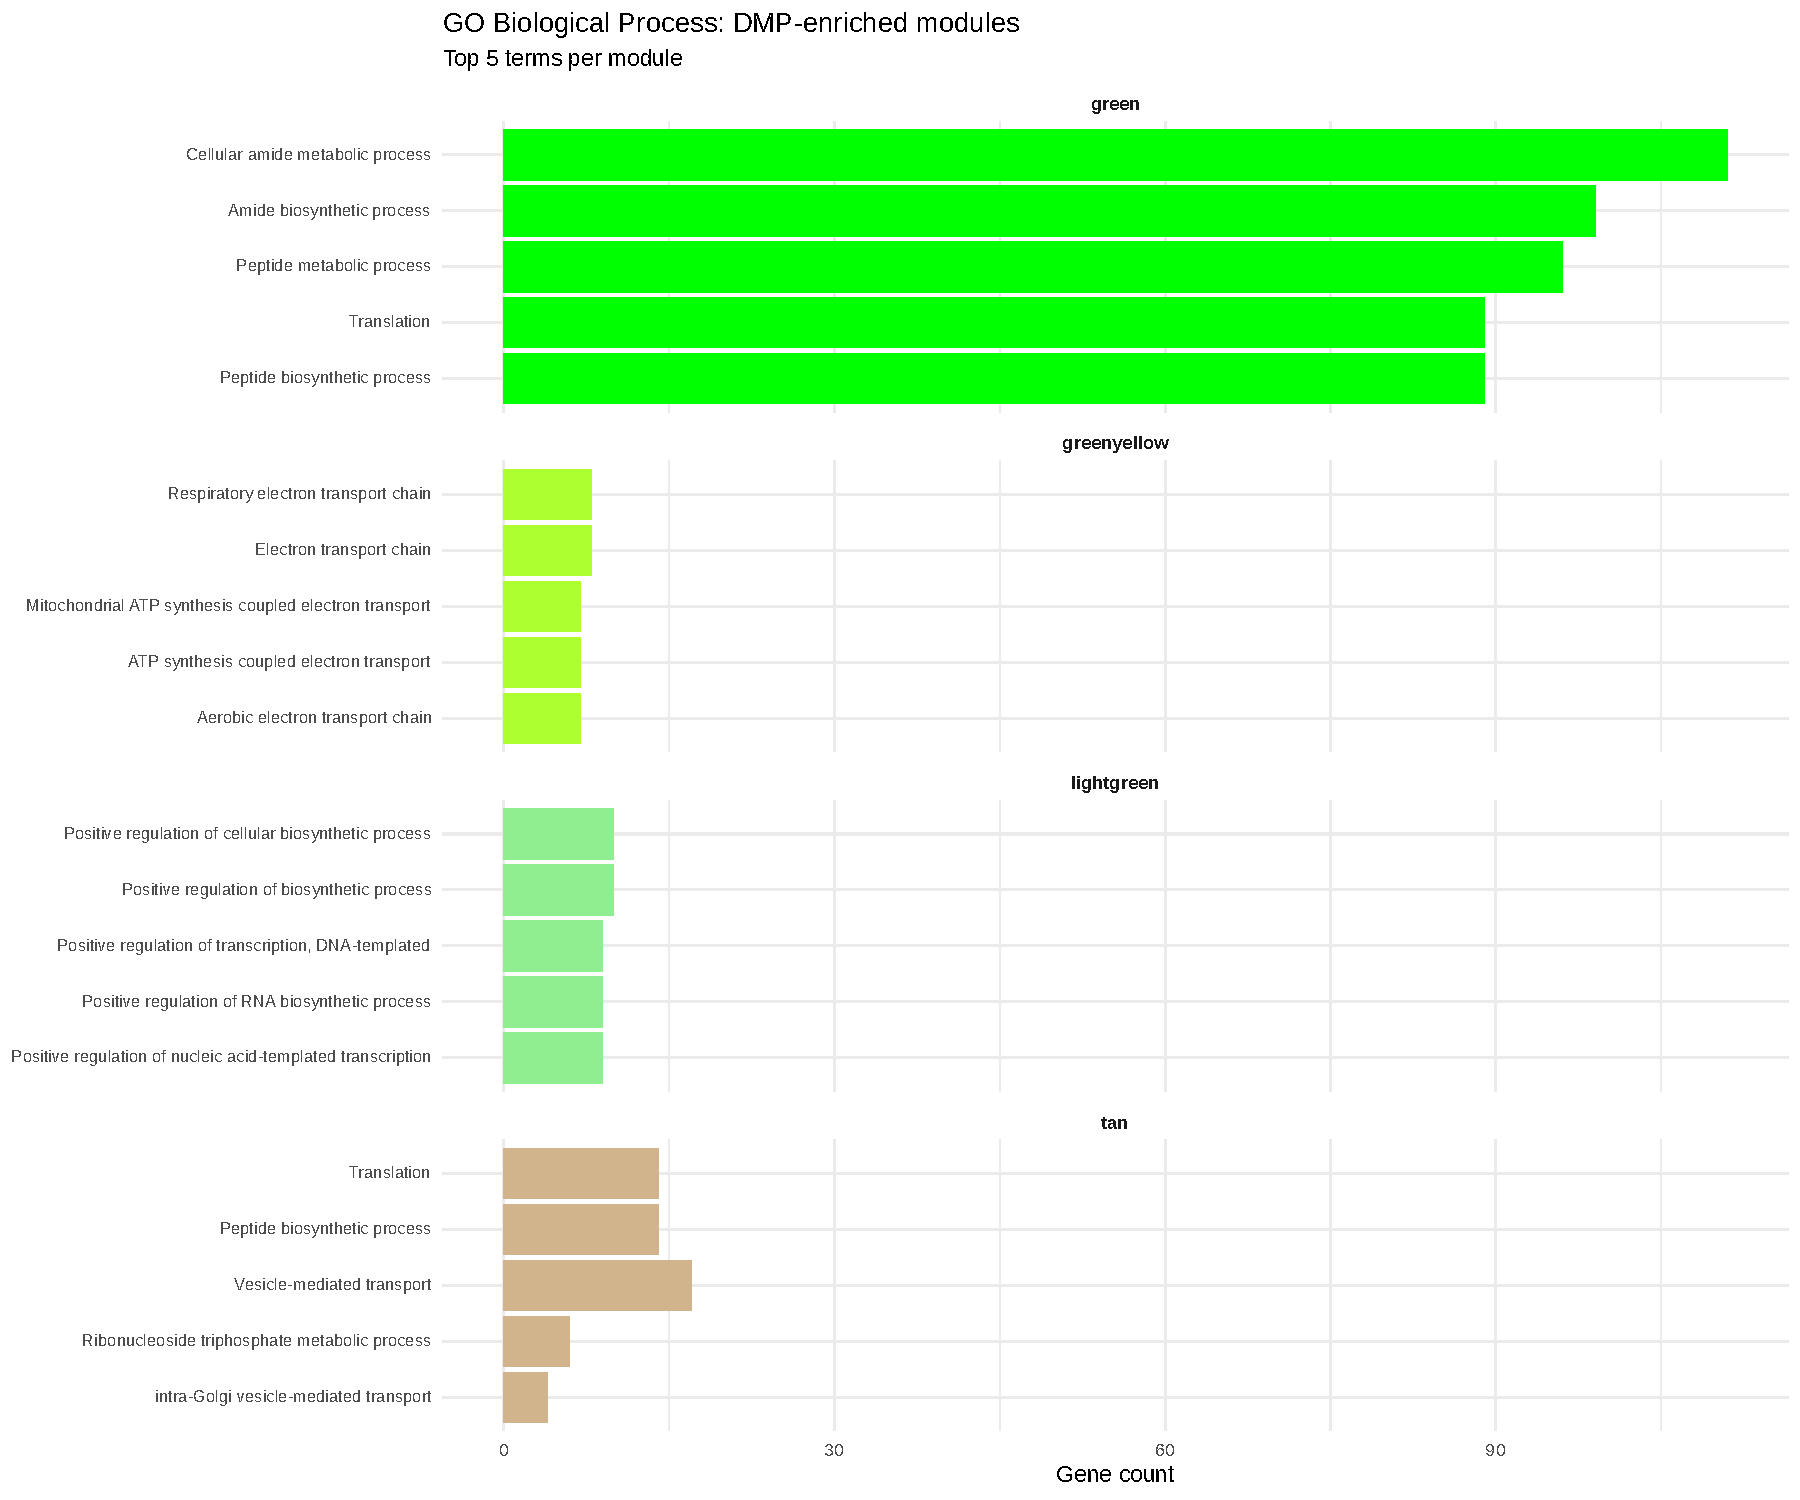
\includegraphics[width=\textwidth]{fig8i_module_go_enrichment.pdf}
        \caption{}
    \end{subfigure}

    \caption{\textbf{Differentially methylated genes are enriched in tissue-specific co-expression modules.}
    (\textbf{A}) Scale-free topology fit and mean connectivity for soft-thresholding power selection (power = 12).
    (\textbf{B}) Gene dendrogram and module assignment from WGCNA.
    (\textbf{C}) Module--trait correlation heatmap using tissue$\times$condition interaction terms (e.g., tail\_control, tail\_amputated, eye\_control, eye\_amputated).
    (\textbf{D}) DMP burden per WGCNA module (\% of genes with DMPs).
    (\textbf{E}) Fisher's exact test for DMP enrichment across modules ($-\log_{10}$ adjusted $p$-value).
    (\textbf{F}) Gene Ontology enrichment of DMP-enriched modules.}
    \label{fig:wgcna}
\end{figure}


%%%%%%%%%%%%%%%%%%%%%%%%%%%%%%%%%%%%%%%%%%%%%%%%%%%%%%%%%%%%%%%%%%%%%%%%%%%
%% DISCUSSION
%%%%%%%%%%%%%%%%%%%%%%%%%%%%%%%%%%%%%%%%%%%%%%%%%%%%%%%%%%%%%%%%%%%%%%%%%%%

\section*{Discussion}

The data presented here provide one of the first comprehensive descriptions of a gastropod methylome and, to our knowledge, the first characterization of methylation dynamics during regeneration in any mollusk. Three principal findings emerge. First, \textit{D.\ laeve} possesses a mosaic methylome dominated by gene-body methylation, with hypomethylated promoters and a promoter CpG architecture lacking canonical CpG islands---consistent with the pattern described in other invertebrates but now extended to a terrestrial gastropod capable of complex tissue regeneration. Second, the organism's epigenetic toolkit retains DNMT1, TET2, and TET3 but has lost DNMT3 and DNMT2, indicating that methylation in \textit{D.\ laeve} is maintained replicatively but cannot be established through the canonical \textit{de novo} pathway. Third, tail amputation induces 17,729 reproducible methylation changes that are functionally enriched for morphogenesis and ciliary assembly programs, yet these changes show no correlation with transcriptional changes at the gene level ($\rho = 0.009$, $p = 0.55$). Instead, differentially methylated genes are concentrated in co-expression modules associated with specific tissue identities, suggesting that the methylation signal may reflect cell-type compositional shifts during blastema formation.

The mosaic methylation pattern of \textit{D.\ laeve}---gene bodies methylated, promoters hypomethylated, transposable elements moderately and context-dependently methylated---aligns with what has been described in arthropods, cnidarians, and other mollusks \cite{sardaEvolutionInvertebrateGene2012, haidarDNAMethylationMachinery2024}. The dominance of intermediate-CpG promoters (85.1\% ICP, 14.9\% LCP, 0.1\% HCP by Weber classification) and the absence of a bimodal promoter CpG distribution distinguish this genome from vertebrates, where high-CpG-density promoters associated with CpG islands are a defining feature \cite{gardiner-gardenCpGIslandsVertebrate1987}. The metagene profiles further confirm the exonic enrichment of methylation, with a clear exon--intron oscillation in multi-exon genes that disappears in intronless genes, consistent with reports from honeybees and oysters. The positive correlation between baseline gene body methylation and expression ($\rho = 0.407$) is noteworthy: this relationship, while robust at baseline, is entirely absent for differential changes during regeneration, indicating that the correlation reflects a static feature of the epigenome rather than a dynamic regulatory mechanism.

The absence of DNMT3 is the most striking feature of the \textit{D.\ laeve} methylation toolkit and is shared with several other invertebrate lineages \cite{pongerEvolutionaryDiversificationDNA2005, haidarDNAMethylationMachinery2024}. This raises a fundamental question: how are new methylation patterns established during development or regeneration in an organism that can only maintain existing marks? Several non-mutually exclusive explanations are possible. First, DNMT1 may itself possess low-level \textit{de novo} activity, as recently demonstrated in mouse embryonic stem cells where DNMT1 methylates retrotransposons in a UHRF1-dependent manner at H3K9me3-marked loci \cite{haggertyDnmt1HasNovo2021}. The duplication of UHRF1 in \textit{D.\ laeve} may be relevant in this context. Second, methylation patterns may be inherited maternally through the oocyte, with DNMT1 faithfully propagating a pre-established landscape. Third, TET2- and TET3-mediated demethylation, rather than \textit{de novo} methylation, may be the primary mechanism through which the methylation landscape is dynamically reshaped during regeneration.

The most unexpected finding is the near-complete decoupling of methylation changes from transcriptional changes during early regeneration. In the mammalian paradigm, differentially methylated regions---particularly at promoters and enhancers---are expected to correlate with changes in gene expression. In \textit{D.\ laeve}, the Spearman correlation between per-gene methylation change and expression change is essentially zero, regardless of whether the analysis is restricted to promoters ($\rho = 0.015$), exons ($\rho = -0.001$), introns ($\rho = 0.003$), or intergenic regions ($\rho = 0.005$). This result may reflect several non-exclusive possibilities. The methylation changes may be consequential rather than causal---downstream of cell-type compositional shifts during blastema formation rather than drivers of transcriptional reprogramming. Alternatively, methylation may affect post-transcriptional processes such as alternative splicing or transcript stability. A third possibility is that the methylation changes observed at 2~dpa are preparatory, establishing a chromatin context that will enable transcriptional changes at later stages. Finally, recent work using nanopore sequencing in humans has demonstrated that much of the apparent correlation between CpG methylation and gene expression in mammalian systems is driven by underlying sequence variants rather than by methylation directly \cite{stefanssonCorrelationCpGMethylation2024}.

The enrichment of DMPs in specific WGCNA modules---particularly modules associated with the ovotestis transcriptome and with morphogenesis---offers a more nuanced interpretation than the gene-level null result. Because co-expression modules often correspond to cell-type-specific transcriptional programs, the non-random concentration of DMPs in tissue-identity modules is consistent with the hypothesis that blastema formation involves an expansion of cell populations whose methylation profiles differ from differentiated tail tissue. Single-cell methylation profiling would be needed to distinguish cell-type compositional effects from within-cell epigenetic reprogramming.

The TE methylation data add another dimension. In mammals, TEs are heavily methylated as a primary silencing strategy. In \textit{D.\ laeve}, TE methylation is moderate and strongly dependent on genomic context: TEs overlapping gene bodies are more methylated than intergenic TEs, consistent with passive acquisition of methylation from the surrounding gene-body domain rather than targeted silencing. Without DNMT3, \textit{D.\ laeve} may lack the capacity for \textit{de novo} silencing of newly inserted TEs. Alternative defense mechanisms may include the piRNA pathway or chromatin-based silencing through histone modifications independent of DNA methylation.

Several limitations should be noted. The sample size is small ($n = 2$ per condition for WGBS). WGBS and RNA-seq were performed on separate biological replicates, limiting paired correlation. Only a single post-amputation time point was examined (2~dpa). The absence of ATAC-seq or histone modification data prevents assessment of the broader chromatin context. WGBS alone cannot distinguish passive from active demethylation; oxidative bisulfite sequencing would be needed.

Future work should address these limitations through time-course WGBS, paired WGBS and RNA-seq, and ATAC-seq to integrate methylation with chromatin accessibility. Pharmacological or genetic perturbation of TET2/TET3 activity during regeneration would provide direct evidence for or against a causal role of active demethylation in blastema formation.


%%%%%%%%%%%%%%%%%%%%%%%%%%%%%%%%%%%%%%%%%%%%%%%%%%%%%%%%%%%%%%%%%%%%%%%%%%%
%% MATERIALS AND METHODS
%%%%%%%%%%%%%%%%%%%%%%%%%%%%%%%%%%%%%%%%%%%%%%%%%%%%%%%%%%%%%%%%%%%%%%%%%%%

\section*{Materials and Methods}

\subsection*{Experimental design}

The objective of this study was to characterize the DNA methylation landscape of \textit{Deroceras laeve} tail tissue and to identify methylation changes associated with early regeneration. Adult \textit{D.\ laeve} slugs were maintained under standard laboratory conditions at the Institute of Neurobiology, UNAM, Juriquilla, Quer\'{e}taro, Mexico. For the amputation group, tail tissue posterior to the mantle was removed with a sterile scalpel, and animals were allowed to regenerate for two days, corresponding to the blastema formation stage. Control animals were age-matched and underwent identical handling without amputation. Tissue was collected from $n = 2$ control animals (C1, C2) and $n = 2$ amputated animals (A1, A2).

\subsection*{DNA extraction and whole-genome bisulfite sequencing}

Genomic DNA was extracted from tail tissue using a commercial kit following the manufacturer's protocol. DNA was assessed for quantity and integrity by fluorometry and agarose gel electrophoresis. Bisulfite conversion was performed with an appropriate conversion kit, and sequencing libraries were prepared according to standard WGBS protocols. Libraries were sequenced on an Illumina platform to obtain sufficient genome-wide CpG coverage for downstream differential methylation analysis.

\subsection*{RNA extraction and RNA-seq}

Total RNA was extracted from separate biological replicates across six tissues---tail (control and amputated), eye (control and amputated), body wall (control, irradiated, and fungicide-exposed), head, juvenile, and ovotestis---using a commercial RNA extraction kit. RNA quality was assessed by spectrophotometry and capillary electrophoresis. Strand-specific RNA-seq libraries were prepared and sequenced on an Illumina platform. Note that RNA-seq and WGBS were performed on independent biological samples, precluding direct paired correlation of methylation and expression within individual animals.

\subsection*{Bioinformatic analyses}

\subsubsection*{Genome and annotation.}
All analyses used the \textit{D.\ laeve} \textit{de novo} genome assembly (1.78~Gb, 31 chromosomes, 42.99\% GC) and EviAnn gene annotation. Analysis was restricted to chromosomes 1--31; HiC scaffolds were excluded. Repetitive elements were annotated using RepeatMasker with the Dfam database, and Kimura 2-parameter divergence values were computed for each TE copy as a proxy for evolutionary age.

\subsubsection*{WGBS processing.}
Raw reads were trimmed for adapters and low-quality bases using Trim Galore. Trimmed reads were aligned to the bisulfite-converted reference genome using Bismark, followed by deduplication and methylation extraction. Per-CpG methylation levels ($\beta$ values) were computed as the ratio of methylated reads to total reads at each CpG site. Strand collapse was performed: minus-strand CpG positions were shifted by $-1$~bp and counts summed with the corresponding plus-strand position, yielding one measurement per CpG dinucleotide. Sites with fewer than 5$\times$ coverage in any of the four samples were excluded, yielding 25,439,068 CpGs from a genome total of 45,535,149.

\subsubsection*{Dinucleotide and CpG landscape analysis.}
Dinucleotide frequencies were computed genome-wide and compared to expected frequencies derived from mononucleotide composition. CpG observed/expected ratios, CpG density, and GC content were calculated in 1-kb sliding windows.

\subsubsection*{Promoter CpG classification.}
Promoter regions were defined as $\pm$1~kb around the annotated transcription start site. Promoters were classified following the Weber criteria \cite{weberDistributionSilencingPotential2007}: high-CpG-density promoters (HCP; CpG O/E $\geq$ 0.75 and GC content $\geq$ 55\%), low-CpG-density promoters (LCP; CpG O/E $<$ 0.48), and intermediate-CpG-density promoters (ICP; all others).

\subsubsection*{Metagene methylation profiles.}
For each gene, four segments were defined: distal upstream (5--2~kb from TSS), promoter (2~kb upstream of TSS), gene body, and downstream (5~kb from TTS). Each segment was divided into 20 equal-length bins. Mean methylation was computed per bin per gene and aggregated by expression group (quartiles, quintiles, or deciles from RNA-seq) and by gene architecture (single-exon, two-exon, three or more exons). Profiles were computed separately for control and amputated samples.

\subsubsection*{TE methylation analysis.}
Mean methylation was computed per RepeatMasker-annotated TE copy. TEs were stratified by superfamily (DNA, LTR, LINE, SINE, RC, Unknown) and by genomic context (overlapping gene bodies vs.\ intergenic, defined by overlap with annotated gene bodies using GenomicRanges).

\subsubsection*{Differential methylation analysis.}
Differentially methylated positions (DMPs) and differentially methylated regions (DMRs) were identified using the DSS package in R, which employs a beta-binomial regression framework with smoothing and an empirical Bayes approach for variance estimation. DMPs were called at FDR $< 0.05$ with $|\Delta\beta| > 10\%$. DMPs and DMRs were annotated to genomic features (Promoter $>$ Exon $>$ Intron $>$ Intergenic, mutually exclusive) using GenomicRanges \texttt{findOverlaps()}.

\subsubsection*{RNA-seq processing and differential expression.}
Gene-level read counts were quantified using HTSeq. Gene filtering required $\geq$10 counts in at least the minimum group size per tissue. Variance-stabilizing transformation (VST) was applied for visualization and WGCNA. Differential expression between control and amputated tail samples was assessed using DESeq2 with apeglm log$_2$ fold-change shrinkage and Benjamini--Hochberg correction (padj $< 0.05$). Within-group outlier detection was performed by centroid distance in PCA space: samples with distance $> 2\times$ the within-tissue median were flagged.

\subsubsection*{Methylation machinery identification.}
A curated list of 26 methylation-related genes (18 present, 8 absent) was assembled through BLAST and HMMER searches of the predicted \textit{D.\ laeve} proteome against reference sequences from \textit{Homo sapiens}, \textit{Mus musculus}, \textit{Apis mellifera}, and \textit{Crassostrea gigas}. Domain architecture was confirmed using InterPro. Gene-level expression of identified candidates was extracted from the multi-tissue RNA-seq dataset (VST-normalized).

\subsubsection*{WGCNA.}
Weighted gene co-expression network analysis was performed using the WGCNA R package on VST-normalized expression data from all six tissues. Genes in the bottom 25\% by variance were filtered. A signed adjacency matrix was computed using soft-thresholding power 12. Modules were detected using dynamic tree cutting of the topological overlap matrix dendrogram (minimum module size = 50, merge cut height = 0.25). Module eigengenes were correlated with tissue$\times$condition interaction traits (e.g., tail\_control, tail\_amputated, eye\_control, eye\_amputated) using Pearson correlation. DMP enrichment per module was assessed using one-sided Fisher's exact test with Benjamini--Hochberg correction. Module membership vs.\ gene significance scatter plots were computed for the top modules. Module-level Gene Ontology enrichment was performed using clusterProfiler with STRING-derived GO annotations.

\subsubsection*{Gene Ontology and pathway enrichment.}
GO enrichment of DMP- and DMR-associated genes was performed using clusterProfiler with Benjamini--Hochberg correction. Biological Process, Cellular Component, and Molecular Function ontologies were tested. KEGG and Reactome pathway enrichment were performed as complementary analyses, using STRING protein enrichment terms mapped to \textit{D.\ laeve} gene IDs via orthology.

\subsection*{Statistical analysis}

All statistical analyses were performed in R (v4.5). Spearman rank correlation was used to assess the relationship between per-gene methylation change and expression change across genomic regions. PCA of per-CpG methylation values was performed using \texttt{prcomp}. Multiple testing correction was applied using the Benjamini--Hochberg procedure throughout (adjusted $p < 0.05$). Fisher's exact test was used for module-level DMP enrichment with BH correction. All analysis code is deposited at \url{https://github.com/somnasgarden/Deroceras-Leave}.


%%%%%%%%%%%%%%%%%%%%%%%%%%%%%%%%%%%%%%%%%%%%%%%%%%%%%%%%%%%%%%%%%%%%%%%%%%%
%% REFERENCES
%%%%%%%%%%%%%%%%%%%%%%%%%%%%%%%%%%%%%%%%%%%%%%%%%%%%%%%%%%%%%%%%%%%%%%%%%%%

\bibliography{references}


%%%%%%%%%%%%%%%%%%%%%%%%%%%%%%%%%%%%%%%%%%%%%%%%%%%%%%%%%%%%%%%%%%%%%%%%%%%
%% ACKNOWLEDGMENTS
%%%%%%%%%%%%%%%%%%%%%%%%%%%%%%%%%%%%%%%%%%%%%%%%%%%%%%%%%%%%%%%%%%%%%%%%%%%

\section*{Acknowledgments}

\paragraph{Funding:}
% TODO: Insert funding sources with grant numbers and recipient initials.

\paragraph{Author contributions:}
Conceptualization: RLT, JRMR\\
Methodology: RLT, WGS, MSTA\\
Investigation: RLT, WGS\\
Formal analysis: RLT\\
Visualization: RLT\\
Supervision: JRMR, AVE\\
Writing---original draft: RLT\\
Writing---review \& editing: RLT, WGS, MSTA, AVE, JRMR

\paragraph{Competing interests:}
The authors declare that they have no competing interests.

\paragraph{Data and materials availability:}
All sequencing data have been deposited at [accession numbers]. Analysis code is available at \url{https://github.com/somnasgarden/Deroceras-Leave}. All other data needed to evaluate the conclusions of this paper are present in the main text or the supplementary materials.


%%%%%%%%%%%%%%%%%%%%%%%%%%%%%%%%%%%%%%%%%%%%%%%%%%%%%%%%%%%%%%%%%%%%%%%%%%%
%% SUPPLEMENTARY MATERIALS
%%%%%%%%%%%%%%%%%%%%%%%%%%%%%%%%%%%%%%%%%%%%%%%%%%%%%%%%%%%%%%%%%%%%%%%%%%%

\newpage
\section*{Supplementary Materials}

% fig. S1 — Transcriptome QC: sample dendrogram, PCA, correlation heatmap (batch 0.5)
% fig. S2 — TE CpG density, O/E, and GC distributions (batch 01: fig1e–1g)
% fig. S3 — Promoter CpG classification: Weber histogram, O/E vs GC scatter, class proportions, metagene by class, gene structure by class (batch 03)
% fig. S4 — Metagene profiles at quartile and quintile resolution; 2-exon gene class; ncRNA (batch 04)
% fig. S5 — Regional methylation-expression: decile boxplots, expanded region correlations (batch 04: fig4h, fig4l)
% fig. S6 — DMP/DMR annotation: annotation pies, direction by region, enrichment tests (batch 06: fig6e-6i)
% fig. S7 — DMP and DMR heatmaps with gene names (batch 06: fig6h, 6i)
% fig. S8 — Methylation-expression decoupling: expanded region correlations, DMP/DMR location (batch 07: fig7f-7i)
% fig. S9 — WGCNA: sample dendrogram, eigengene boxplots, module sizes, Wilcoxon test, MM vs GS, eigengene network (batch 08)
% fig. S10 — TF/motif/GENIE3 integration: motif enrichment, TF class sensitivity, concordant loci (batch 09)
% fig. S11 — Methylation entropy: distribution, regional, DMP vs. matched, mutual information, entropy metagene (batch 10, 13)
% fig. S12 — PCA and Manhattan plots of DM analysis (batch 06: fig6a, 6c)
%
% table S1 — Bisulfite conversion rates and WGBS coverage statistics per sample
% table S2 — Full list of 26 methylation machinery genes with domain annotations and expression
% table S3 — Complete DMP and DMR lists with genomic coordinates and annotations
% table S4 — WGCNA module assignments, hub genes, and Fisher enrichment
% table S5 — Full GO/KEGG/Reactome enrichment results
% table S6 — Concordant DMP/DE gene list (228 genes with >=3 DMPs and padj < 0.05)

\end{document}
